%%%%%%%%%%%%%%%%%%%%%%%%%%%%%%%%%%%%%%%%%%%%%%%%%%%%%%%%%%%%%%%%%%%%%%%%%%%%%%%%
%   Copyright 2016, KAIST.
%   All rights reserved.
%
%   Use is subject to license terms.
%
%   This distribution may include materials developed by third parties.
%%%%%%%%%%%%%%%%%%%%%%%%%%%%%%%%%%%%%%%%%%%%%%%%%%%%%%%%%%%%%%%%%%%%%%%%%%%%%%%%

\documentclass[oneside,openany]{book}
\usepackage{url, amssymb, amsmath, amsthm, stmaryrd, xspace}
\usepackage{amsfonts, graphicx, fullpage, times, wrapfig}
\usepackage{hyperref, array, color,anysize,ifpdf,tikz}

\newif\ifrelease
\ifx\release\undefined
  \releasefalse
\else
  \releasetrue
\fi

% Please uncomment the following line for a release version.
% -- Sukyoung
%\releasetrue

\parskip = 7pt plus 2pt minus 1pt
\makeatletter
\setlength\partopsep{4\p@ \@plus 1\p@}
\def\@listi{\leftmargin\leftmargini
            \parsep\parskip
            \topsep 0\p@
            \itemsep\topsep}
\let\@listI\@listi
\@listi
\def\@listii {\leftmargin\leftmarginii
              \labelwidth\leftmarginii
              \advance\labelwidth-\labelsep}
\def\@listiii{\leftmargin\leftmarginiii
              \labelwidth\leftmarginiii
              \advance\labelwidth-\labelsep}
\makeatother
\parindent = 0pt

\setcounter{tocdepth}{1}

\ifpdf
  \usepackage{epic,eepicemu}
\else
  \usepackage{epic,eepic}
\fi

\newcommand{\lit}{lit}
\newcommand{\safe}{SAFE\xspace}
% thicker vertical line
\newcolumntype{?}{!{\vrule width 1pt}}

% Styles
\definecolor{dkgreen}{rgb}{0,0.6,0}
\definecolor{gray}{rgb}{0.5,0.5,0.5}
\definecolor{mauve}{rgb}{0.58,0,0.82}
\lstdefinelanguage{JavaScript}{
  keywords={async, await, break, case, catch, class, const, continue, debugger,
    default, delete, do, else, enum, export, extends, false, finally, for,
    function, if, import, in, instanceof, new, null, return, super, switch, this,
    throw, true, try, typeof, var, void, while, with, yield},
  keywordstyle=\color{blue}\bfseries,
  ndkeywordstyle=\color{darkgray}\bfseries,
  identifierstyle=\color{black},
  sensitive=false,
  comment=[l]{//},
  morecomment=[s]{/*}{*/},
  commentstyle=\color{dkgreen}\ttfamily,
  stringstyle=\color{purple}\ttfamily,
  morestring=[b]',
  morestring=[b]"
}
\lstdefinestyle{myJSstyle}{
  language=JavaScript,
  numbers=left,
  stepnumber=1,
  extendedchars=true,
  basicstyle=\footnotesize\ttfamily,
  showstringspaces=false,
  showspaces=false,
  tabsize=2,
  breaklines=true,
  showtabs=false,
  captionpos=b
}

% Basic
\DeclareMathAlphabet{\mathpzc}{T1}{pzc}{m}{it}
\newcommand{\powerset}[1]{\mathcal{P}(#1)}
\newcommand{\imbox}[1]{\mbox{\small \textit{#1}}}
\newcommand{\name}[1]{\textsf{#1}}
\newcommand{\inred}[1]{{\color{red}{#1}}}
\newcommand{\todo}{\inred{TODO}}
\newcommand{\abs}[1]{{#1}^{\#}}
\newcommand{\finmap}{{\xrightarrow[]{\text{fin}}}}
\newcommand{\mapstos}{\;\dot{\mapsto}\;}
\newcommand{\Dom}{\name{Dom}}

% Tool
\newcommand{\tool}{\text{SAFE}_\name{DS}}

% Keywords
\newcommand{\jscode}[1]{\text{\lstinline[style=myJSstyle,numbers=none]!#1!}}
\newcommand{\code}[1]{\texttt{#1}}
\newcommand{\kwif}{\code{if}}
\newcommand{\kwelse}{\code{else}}
\newcommand{\kwret}{\code{ret}}
\newcommand{\kwobj}{\code{\{\}}}
\newcommand{\kwtrue}{\code{true}}
\newcommand{\kwfalse}{\code{false}}

% Notations
\newcommand{\prog}{P}
\newcommand{\labset}{\mathcal{L}}
\newcommand{\lab}{\mathpzc{l}}
\newcommand{\labdot}[1]{{{\bullet_{\lab_{#1}}}}}
\newcommand{\ilab}{\lab_\iota}
\newcommand{\labnext}{\name{next}}
\newcommand{\op}{\name{op}}
\newcommand{\ops}{\dot{\name{op}}}
\newcommand{\inst}{i}
\newcommand{\expr}{e}
\newcommand{\refer}{r}

% Numbers
\newcommand{\numset}{\mathbb{N}}

% States
\newcommand{\stset}{\mathbb{S}}
\newcommand{\st}{\sigma}
\newcommand{\istset}{\stset_\iota}
\newcommand{\ist}{\st_\iota}

% Memories
\newcommand{\memset}{\mathcal{M}}
\newcommand{\absmemset}{\abs{\memset}}
\newcommand{\mem}{M}
\newcommand{\absmem}{\abs{\mem}}

% Contexts
\newcommand{\ctxtset}{\mathbb{C}}
\newcommand{\absctxtset}{\abs{\ctxtset}}
\newcommand{\ctxt}{c}
\newcommand{\absctxt}{\abs{\ctxt}}
\newcommand{\eabsctxt}{\absctxt_\name{env}}

% Transition Relations
\newcommand{\trans}{\leadsto}
\newcommand{\rutrans}{%
            \mathrel{\raisebox{.1em}{%
            \rotatebox[origin=c]{30}{$\trans$}}}}
\newcommand{\rdtrans}{%
            \mathrel{\raisebox{.1em}{%
            \rotatebox[origin=c]{-30}{$\trans$}}}}


% Complete Lattice
\newcommand{\join}{\sqcup}
\newcommand{\meet}{\sqcap}
\newcommand{\bigjoin}{\bigsqcup}
\newcommand{\bigmeet}{\bigsqcap}
\newcommand{\order}{\sqsubseteq}

% Concrete Domains
\newcommand{\dom}{\mathbb{D}}
\newcommand{\elem}{d}
\newcommand{\ielem}{\elem_\iota}

% Abstract Domains
\newcommand{\absdom}{\abs{\dom}}
\newcommand{\abselem}{\abs{\elem}}
\newcommand{\iabselem}{\abs{\elem}_\iota}

% Concrete Semantics
\newcommand{\sem}[1]{[\![{#1}]\!]}
\newcommand{\transfer}{F}
\newcommand{\step}{\name{step}}

% Abstract Semantics
\newcommand{\abssem}[1]{\abs{\sem{#1}}}
\newcommand{\abstransfer}{\abs{\transfer}}
\newcommand{\absstep}{\abs{\step}}

% Abstract Sensitivity
\newcommand{\viewmap}{\delta}
\newcommand{\sabsdom}{\absdom_\viewmap}
\newcommand{\sabselem}{{\abselem_\viewmap}}
\newcommand{\viewset}{\Pi}
\newcommand{\view}{\pi}
\newcommand{\sabsstep}{\absstep_\viewmap}
\newcommand{\viewtrans}[2]{\abssem{#1 \rightarrow #2}}

% Flow Sensitivity
\newcommand{\fs}{\name{FS}}
\newcommand{\fsviewmap}{\viewmap^\fs}

% Locations
\newcommand{\locset}{\mathbb{L}}
\newcommand{\loc}{l}
\newcommand{\abslocset}{\abs\locset}
\newcommand{\absloc}{\abs\loc}

% Variables
\newcommand{\varset}{\mathbb{X}}
\newcommand{\varx}{\code{x}}

% Values
\newcommand{\valset}{\mathbb{V}}
\newcommand{\val}{v}
\newcommand{\pvalset}{\valset_\name{p}}
\newcommand{\pval}{\val_\name{p}}
\newcommand{\fvalset}{\mathbb{F}}
\newcommand{\fval}[2]{\lambda #1. #2}
\newcommand{\strset}{\valset_\name{str}}
\newcommand{\str}{\val_\name{str}}
\newcommand{\absvalset}{\abs{\valset}}
\newcommand{\absval}{\abs{\val}}

\newcommand{\valgamma}{\gamma_\val}

% Addresses
\newcommand{\addrset}{\mathbb{A}}
\newcommand{\eaddrset}{\addrset_\name{env}}
\newcommand{\oaddrset}{\addrset_\name{obj}}
\newcommand{\addr}{a}
\newcommand{\tladdr}{\addr_{\name{top}}}
\newcommand{\absaddrset}{\abs{\addrset}}
\newcommand{\absaddr}{\abs{\addr}}
\newcommand{\eabsaddr}{\absaddr_\name{env}}
\newcommand{\rabsaddr}{\absaddr_\name{ret}}
\newcommand{\oabsaddr}{\absaddr_\name{obj}}

% Abstract Counting
\newcommand{\abscount}{\abs{n}}
\newcommand{\inc}{\name{inc}}
\newcommand{\abscountset}{\abs{\mathbb{N}}}
\newcommand{\abszero}{\abs{0}}
\newcommand{\absone}{\abs{1}}
\newcommand{\absmany}{\abs{\geq\!\!2}}

% Sealed Symbolic Interpretation
\newcommand{\symb}{\omega}
\newcommand{\symbset}{\Omega}
\newcommand{\symbolic}[1]{{#1}_\symb}
\newcommand{\symbstset}{\symbolic{\stset}}
\newcommand{\symbst}{\symbolic{\st}}
\newcommand{\nsymbst}[1]{\st_{\symb,#1}}
\newcommand{\symbmemset}{\symbolic{\memset}}
\newcommand{\symbtrans}{\symbolic{\trans}}
\newcommand{\excst}{\bot}
\newcommand{\symbevt}{\symb_\jscode{evt}}
\newcommand{\symbint}{\symb_\jscode{int}}

% Combined Analysis
\newcommand{\comb}[1]{\widetilde{#1}}
\newcommand{\combdom}{\comb{\dom}}
\newcommand{\combelem}{\comb{\elem}}
\newcommand{\combgamma}{\comb{\gamma}}
\newcommand{\combstep}{\comb{\step}}
\newcommand{\combtransfer}{\comb{\transfer}}
\newcommand{\sgamma}{\gamma_\viewmap}
\newcommand{\converter}{\tau}
\newcommand{\saconverter}{\abs{\converter}}
\newcommand{\asconverter}{\symbolic{\converter}}
\newcommand{\combviewtrans}[2]{\sem{\comb{#1 \rightarrow #2}}}

\newcommand{\symbdom}{\symbolic{\dom}}
\newcommand{\symbelem}{\symbolic{\elem}}
\newcommand{\symbgamma}{\symbolic{\gamma}}
\newcommand{\symbstep}{\symbolic{\step}}

% Legacy
\newcommand{\scombstep}{\comb{\step}_\viewmap}
\newcommand{\scombgamma}{\combgamma_\viewmap}
\newcommand{\scombelem}{\comb{\elem}_\viewmap}

% Triage
\newcommand{\triage}{\name{triage}}
\newcommand{\atriage}{\triage_\aelem}

% Rules
\newcommand{\referrule}[3]{#1 \vdash_\refer #2 \Rightarrow  #3}
\newcommand{\exprrule}[3]{#1 \vdash_\expr #2 \Rightarrow #3}

% Abstract Semantics
\newcommand{\referabssem}[1]{\abssem{#1}_\refer}
\newcommand{\exprabssem}[1]{\abssem{#1}_\expr}

% Identity function
\newcommand{\identity}{\name{id}}

% Checker
\newcommand{\checker}{\name{checker}}

% Concerto
\newcommand{\concerto}{\textsc{Concerto}}

% Table 1
\newcommand{\myhead}[3]{
  \multicolumn{1}{c|}{\textbf{#1}} &
  \multicolumn{1}{c|@{~}}{\textbf{#2}} &
  \multicolumn{4}{@{~}c@{~}?}{\textbf{#3}} &
  \multicolumn{1}{c|}{\textbf{#1}} &
  \multicolumn{1}{c|@{~}}{\textbf{#2}} &
  \multicolumn{4}{@{~}c@{~}?}{\textbf{#3}} &
  \multicolumn{1}{c|}{\textbf{#1}} &
  \multicolumn{1}{c|@{~}}{\textbf{#2}} &
  \multicolumn{4}{@{~}c@{~}}{\textbf{#3}}\\\hline
}
\newcommand{\mydata}[6]{
  \multirow{#1}{*}{\jscode{#2}} &
  \jscode{#3} &
  \text{#4} &
  \text{/} &
  \text{#5} &
  \text{(#6\%)}
}
\newcommand{\mysucccolor}{yellow}
\newcommand{\mysucc}[6]{
  \multirow{#1}{*}{\jscode{#2}} &
  \multicolumn{1}{>{\columncolor{\mysucccolor}}l|@{~}}    {\jscode{#3}} &
  {\text{#4}} &
  {\text{/}} &
  {\text{#5}} &
  {\text{(#6\%)}}
}
\newcommand{\mymult}[6]{
  \jscode{#2} &
  \multirow{#1}{*}{\jscode{#3}} &
  \multirow{#1}{*}{\text{#4}} &
  \multirow{#1}{*}{\text{/}} &
  \multirow{#1}{*}{\text{#5}} &
  \multirow{#1}{*}{\text{(#6\%)}}
}
\newcommand{\myname}[2]{\multirow{#1}{*}{\jscode{#2}}&&&&&}
\newcommand{\mynewline}[6]{
  \\
  \cline{#1-#2}
  \cline{#3-#4}
  \cline{#5-#6}
}
\newcommand{\mylinef}  {\\\hhline{~|-----}}
\newcommand{\mylineff} {\\\hhline{~|-----~|-----}}
\newcommand{\mylinetf} {\\\hhline{------~|-----}}
\newcommand{\mylinefff}{\\\hhline{~|-----~|-----~|-----}}
\newcommand{\mylinefft}{\\\hhline{~|-----~|-----------}}
\newcommand{\mylineftf}{\\\hhline{~|-----------~|-----}}
\newcommand{\mylineftt}{\\\hhline{~|-----------------}}
\newcommand{\mylinetff}{\\\hhline{------~|-----~|-----}}
\newcommand{\mylinetft}{\\\hhline{------~|-----------}}
\newcommand{\mylinettf}{\\\hhline{------------~|-----}}
\newcommand{\mylinettt}{\\\hhline{------------------}}

% Instantiation Map
\newcommand{\imap}{m}
\newcommand{\imapset}{\mathbb{M}}
\newcommand{\absimap}{\abs{\imap}}
\newcommand{\absimapset}{\abs{\imapset}}
\newcommand{\instant}[2]{#1\!\!\mid\!\!_{#2}}
\newcommand{\imapgamma}{\gamma_\imap}

% Analysis Element
\newcommand{\aelem}{\epsilon}
\newcommand{\aelemset}{\mathbb{E}}
\newcommand{\aelemgamma}{\gamma_{\aelem}}

% Difference Set
\newcommand{\diffset}{\Delta}


\title{{\huge The SAFE Specification}
\\[1em] {\fbox{\LARGE\it Working Draft}}
\\ {\large Version 2.0}
}
\author
{
\begin{tabular}{c}
PLRG @ KAIST
\end{tabular}
}

\begin{document}
\maketitle

\tableofcontents
\section{Overview}

\todo

\chapter{AST}
\small
\[
\begin{array}{llll}
\pgm & ::=  & \fd^*\ \vd^*\ \stmt^* & \mtt{Program(body:~TopLevel)}\\
    &&&\mtt{TopLevel(fds:~List[FunDecl], vds:~List[VarDecl],}\\
&&&\mtt{\phantom{TopLevel(}stmts:~List[SourceElements])}\\

\fd &::=& {\tt function} \ f \verb+(+(x\verb+,+)^*\verb+)+ \ \verb+{+\fd^*\ \vd^*\ \stmt^*\verb+}+
  & \mtt{FunDecl(ftn:~Functional, strict:~Boolean)}\\
&&& \mtt{Functional(fds:~List[FunDecl], vds:~List[VarDecl],}\\
&&&\mtt{\phantom{Functional(}stmts:~SourceElements, name:~Id,}\\
&&&\mtt{\phantom{Functional(}params:~List[Id], body:~String)}\\

\vd &::=& x \ ({\tt =} \ \expr)^? & \mtt{VarDecl(name:~Id, expr:~Option[Expr],}\\
                                       &&& \mtt{\phantom{VarDecl(}strict:~Boolean)}\\

\stmt &::=& \verb+{+\stmt^*\verb+}+ & \mtt{ABlock(stmts:~List[Stmt], internal:~Boolean)}\\
& \mid & {\tt var} \ \vd(\verb+,+ \vd)^* \verb+;+ & \mtt{VarStmt(vds:~List[VarDecl])}\\
& \mid & \verb+;+ & \mtt{EmptyStmt()}\\
& \mid & \expr \verb+;+ & \mtt{ExprStmt(expr:~Expr, internal:~Boolean)}\\
& \mid & {\tt if} \ \verb+(+\expr\verb+)+ \ \stmt \ ({\tt else} \ \stmt)^?
& \mtt{If(cond:~Expr, trueBranch:~Stmt,}\\
&&&\mtt{\phantom{If(}falseBranch:~Option[Stmt])}\\
& \mid &  {\tt switch} \ \verb+(+\expr\verb+)+ \ \verb+{+\cc^* \ ({\tt default} \verb+:+ \stmt^{*})^? \ \cc^* \verb+}+
& \mtt{Switch(cond:~Expr, frontCases:~List[Case],}\\
&&&\mtt{\phantom{Switch(}defopt:~Option[List[Stmt]],}\\
&&&\mtt{\phantom{Switch(}backCases:~List[Case])}\\
& \mid & {\tt do} \ \stmt \ {\tt while} \ \verb+(+\expr\verb+)+ \verb+;+ & \mtt{DoWhile(body:~Stmt, cond:~Expr)}\\
  &\mid& {\tt while} \ \verb+(+\expr\verb+)+ \ \stmt & \mtt{While(cond:~Expr, body:~Stmt)}\\
  &\mid& {\tt for} \ \verb+(+\expr^?\verb+;+ \expr^?\verb+;+ \expr^? \verb+)+ \ \stmt
  & \mtt{For(init:~Option[Expr], cond:~Option[Expr],}\\
&&&\mtt{\phantom{For(}action:~Option[Expr], body:~Stmt)}\\
  &\mid& {\tt for} \ \verb+(+ \lhs \ {\tt in} \ \expr \verb+)+ \ \stmt & 
\mtt{ForIn(lhs:~LHS, expr:~Expr, body:~Stmt)}\\
  &\mid& {\tt for} \ \verb+(+{\tt var} \ \vd(\verb+,+ \vd)^*\verb+;+ \expr^?\verb+;+ \expr^?\verb+)+ \ \stmt
  & \mtt{ForVar(vars:~List[VarDecl], cond:~Option[Expr],}\\
&&&\mtt{\phantom{ForVar(}action:~Option[Expr], body:~Stmt)}\\
  &\mid& {\tt for} \ \verb+(+{\tt var} \ \vd \ {\tt in} \ \expr \verb+)+ \ \stmt & \mtt{ForVarIn(vd:~VarDecl, expr:~Expr, body:~Stmt)}\\
& \mid & {\tt continue} \  \myid^{?} \verb+;+ & \mtt{Continue(target:~Option[Label])}\\
& \mid & {\tt break} \  \myid^{?} \verb+;+ & \mtt{Break(target:~Option[Label])}\\
& \mid & {\tt return} \ \expr^? \verb+;+ & \mtt{Return(expr:~Option[Expr])}\\
& \mid & {\tt with} \ \verb+(+\expr\verb+)+ \ \stmt & \mtt{With(expr:~Expr, stmt:~Stmt)}\\
& \mid & l \; \verb+:+ \; \stmt & \mtt{LabelStmt(label:~Label, stmt:~Stmt)}\\
& \mid & {\tt throw} \ \expr \verb+;+ & \mtt{Throw(expr:~Expr)}\\

& \mid &
{\tt try} \verb+{+\stmt^*\verb+}+ ({\tt catch} \verb+(+\myid\verb+)+ \verb+{+\stmt^*\verb+}+)^? ({\tt finally} \verb+{+\stmt^*\verb+}+)^?
& \mtt{Try(body:~List[Stmt], catchBlock:~Option[Catch],}\\
&&& \mtt{\phantom{Try(}fin:~Option[List[Stmt]])}\\
&&& \mtt{Catch(id:~Id, body:~List[Stmt])}\\
& \mid & {\tt debugger} \verb+;+ & \mtt{Debugger()}\\

\cc &::=& {\tt case} \ \expr \; \verb+:+ \; \stmt^{*} & \mtt{Case(cond:~Expr, body:~List[Stmt])}\\

\expr &::=& \expr\verb+,+ \ \expr & \mtt{ExprList(exprs:~List[Expr])}\\
  &\mid& \expr \ \verb+?+ \ \expr \ \verb+:+ \ \expr & \mtt{Cond(cond:~Expr, trueBranch:~Expr, falseBranch:~Expr)}\\
  &\mid& \expr \ \inop \ \expr & \mtt{InfixOpApp(left:~Expr, op:~Op, right:~Expr)}\\
  &\mid& \preop \ \expr & \mtt{PrefixOpApp(op:~Op, right:~Expr)}\\

  &\mid& \lhs \ \postop & \mtt{UnaryAssignOpApp(lhs:~LHS, op:~Op)}\\
  &\mid& \lhs \ \aop \ \expr & \mtt{AssignOpApp(lhs:~LHS, op:~Op, right:~Expr)}\\
  &\mid& \lhs & \mtt{LHS()}\\
\end{array}
\]

\[
\begin{array}{llll}
\lhs &::=& \lit & \mtt{Literal()}\\
 &\mid& \myid & \mtt{VarRef(id:~Id)}\\
 &\mid& \verb+[+ (\expr^?\verb+,+)^* \ \verb+]+ & \mtt{ArrayExpr(elements:~List[Option[Expr]])}\\
 &\mid& \verb+{+ (\member\verb+,+)^* \verb+}+ & \mtt{ObjectExpr(members:~List[Member]}\\
 &\mid& \verb+(+ \expr \verb+)+ & \mtt{Parenthesized(expr:~Expr)}\\
 & \mid & {\tt function} \ \myid^?  \verb+(+(\myid\verb+,+)^*\verb+)+ \ \verb+{+\fd^*\ \vd^*\ \stmt^*\verb+}+ &
\mtt{FunExpr(ftn:~Functional)}\\
 &\mid& \lhs \verb+[+ \expr \verb+]+ & \mtt{Bracket(obj:~LHS, index:~Expr)}\\
 &\mid& \lhs \verb+.+ \myid & \mtt{Dot(obj:~LHS, member:~Id)}\\
 &\mid& {\tt new} \ \lhs & \mtt{New(lhs:~LHS)}\\
 &\mid& \lhs \verb+(+ (\expr\verb+,+)^* \verb+)+ & \mtt{FunApp(fun:~LHS, args:~List[Expr])} \\ \\

\lit &::=& {\tt this} & \mtt{This()}\\
 &\mid& {\tt null} & \mtt{Null()}\\
 &\mid& {\tt true} & \mtt{Bool(bool:~Boolean)}\\
 &\mid& {\tt false} & \mtt{Bool(bool:~Boolean)}\\
 &\mid& \num & \mtt{DoubleLiteral(text:~String, num:~Double)}\\
&&&\mtt{IntLiteral(intVal:~BigInteger, radix:~Integer)}\\
 &\mid& \str & \mtt{StringLiteral(quote:~String, escaped:~String)}\\
 &\mid& \reg & \mtt{RegularExpression(body:~String, flag:~String)}\\ \\

\member &::=& \prop \ \verb+:+ \ \expr & \mtt{Field(prop:~Property, expr:~Expr)}\\
 &\mid& {\tt get}\ \prop \verb+() {+ \fd^*\ \vd^*\ \stmt^* \verb+}+ 
 & \mtt{GetProp(prop:~Property, ftn:~Functional)}\\
 &\mid& {\tt set}\ \prop \verb+(+ \myid \verb+) {+ \fd^*\ \vd^*\ \stmt^* \verb+}+
 & \mtt{SetProp(prop:~Property, ftn:~Functional)}\\ \\

\prop &::= & \myid & \mtt{PropId(id:~Id)}\\
 &\mid& \str & \mtt{PropStr(str:~String)}\\
 &\mid& \num & \mtt{PropNum(num:~NumberLiteral)}\\
\end{array}
\]

\[
\begin{array}{l@{\;}l@{\;}l@{\;}l@{\;}l@{\;}l@{\;}l@{\;}l@{\;}l@{\;}l@{\;}l@{\;}l@{\;}l@{\;}l@{\;}l@{\;}l@{\;}l@{\;}l@{\;}l@{\;}l@{\;}l@{\;}l@{\;}l@{\;}l@{\;}l@{\;}l@{\;}l@{\;}l@{\;}l@{\;}l@{\;}l@{\;}l@{\;}l@{\;}l@{\;}l@{\;}l@{\;}l@{\;}l@{\;}l@{\;}l@{\;}l@{\;}l@{\;}l@{\;}l@{\;}l@{\;}l@{\;}l}
\aop &::=&
\verb+=+ & \mid &
\verb+*=+ & \mid &
\verb+/=+ & \mid &
\verb+%=+ & \mid &
\verb!+=! & \mid &
\verb+-=+ & \mid &
\verb+[[=+ & \mid &
\verb+>>=+ & \mid &
\verb+>>>=+ & \mid &
\verb+&=+ & \mid &
\verb+^=+ & \mid &
\verb+|=+
\\

\inop &::=& \verb+&&+ & \mid & \verb+||+ & \mid & \verb+|+ & \mid & \verb+&+ & \mid & \verb+^+ & \mid & \verb+[[+ & \mid & \verb+>>+ & \mid & \verb+>>>+ 
 & \mid & \verb!+! & \mid & \verb+-+ & \mid & \verb+*+ & \mid & \verb+/+ & \mid & \verb+%+
 &\mid& \verb+==+ & \mid & \verb+!=+ & \mid & \verb+===+ & \mid & \verb+!==+ & \mid & \verb+[+ & \mid & \verb+>+ & \mid & \verb+[=+
 & \mid & \verb+>=+ \\
 & \mid &
\lefteqn{
 {\tt instanceof} \ \mid \ {\tt in} }\\

\preop &::=& \verb!++! & \mid & \verb+--+ & \mid & \verb+~+ & \mid & \verb+!+ & \mid & \verb!+! & \mid & \verb+-+ & \mid &
\lefteqn{
 {\tt delete} \ \mid \ {\tt void} \ \mid \ {\tt typeof} }\\

\postop &::=& \verb!++! & \mid & \verb+--+\\[1em]

\end{array}
\]

{\inred
\begin{itemize}
\item {\tt VarDecl}: The {\tt expr} field is {\tt None} after {\tt Hoister}.
\item {\tt VarStmt}, {\tt ForVar}, {\tt ForVarIn}: Removed by {\tt Hoister}.
\end{itemize}
}

{\inblue
\begin{itemize}
\item {\tt StmtUnit}: Internally generated statement unit by {\tt Hoister}.
\end{itemize}
}

\chapter{IR}
\small
\[
\begin{array}{llll}
\ir\pgm & ::= & \ir\stmt^* & \mtt{IRRoot(val fds:~List[IRFunDecl], val vds:~List[IRVarStmt],}\\
&&&\mtt{\phantom{IRRoot(}val irs:~List[IRStmt])}\\

\ir\stmt & ::= & \irid \ \verb+=+ \ \ir\expr &
 \mtt{IRExprStmt(val lhs:~IRId, val right:~IRExpr, val ref:~Boolean)}\\

&\mid& \irid \ \verb+=+ \ {\sf delete}\ \irid
& \mtt{IRDelete(val lhs:~IRId, val id:~IRId)}\\

 &\mid& \irid \ \verb+=+ \ {\sf delete}\ \irid\verb+[+\irid\verb+]+
 & \mtt{IRDeleteProp(val lhs:~IRId, val obj:~IRId, val index:~IRExpr)}\\

 &\mid& \irid\verb+[+\irid\verb+] =+ \ \irexpr & \mtt{IRStore(val obj:~IRId, val index:~IRExpr, val rhs:~IRExpr)}\\
 &\mid& \irid \ \verb+=+ \ \verb+{+ (\ir\member\verb+,+)^* \verb+}+
 & \mtt{IRObject(val lhs:~IRId, val members:~List[IRMember],}\\
&&&\mtt{\phantom{IRObject(}val proto:~Option[IRId])}\\
 &\mid& \irid \ \verb+=+ \ \verb+[+ (\irexpr\verb+,+)^* \verb+]+ & \mtt{IRArray(val lhs:~IRId, val elements:~List[Option[IRExpr]])}\\
&&&\mtt{IRArgs(val lhs:~IRId, val elements:~List[Option[IRExpr]])}\\

 &\mid& \irid \ \verb+=+ \ \irid\verb+(+\irid\verb+,+\irid\verb+)+
& \mtt{IRCall(val lhs:~IRId, val fun:~IRId, val thisB:~IRId,}\\
&&&\mtt{\phantom{IRCall(}val args:~IRId)}\\
 &\mid& \irid \ \verb+=+ \ \irid\verb+(+\irid(\verb+,+\irid)^?\verb+)+
& \mtt{IRInternalCall(val lhs:~IRId, val fun:~IRId, val first:~IRExpr,}\\
&&&\mtt{\phantom{IRInternalCall(}val second:~Option[IRId])}\\
&&&{\inblue \mtt{toObject}, \mtt{toNumber}, \mtt{isObject},
\mtt{getBase}, \mtt{iteratorInit},}\\
&&&{\inblue \mtt{iteratorHasNext}, \mtt{iteratorKey}}\\

 &\mid& \irid \ \verb+=+ \ {\sf new}\ \irid\verb+(+(\irid\verb+,+)^*\verb+)+
 & \mtt{IRNew(val lhs:~IRId, val fun:~IRId, val args:~List[IRId])}\\
 &\mid& \irid \ \verb+=+ \ {\sf function} \ \ir{f} \verb+(+\irid\verb+,+\irid\verb+) {+ \ir\stmt^* \verb+}+
& \mtt{IRFunExpr(val lhs:~IRId, val fun:~IRFunctional)}\\
&&&\mtt{IRFunctional(val fromSource:~Boolean, val name:~IRId,}\\
&&&\mtt{\phantom{IRFunctional(}val params:~List[IRId], val args:~List[IRStmt],}\\
&&&\mtt{\phantom{IRFunctional(}val fds:~List[IRFunDecl],}\\
&&&\mtt{\phantom{IRFunctional(}val vds:~List[IRVarStmt], val body:~List[IRStmt])}\\

 &\mid& {\sf function} \ \ir{f} \verb+(+\irid\verb+,+\irid\verb+) {+ \ir\stmt^* \verb+}+
 & \mtt{IRFunDecl(val ftn:~IRFunctional)}\\

 &\mid& \irid \ \verb+=+ \ {\sf eval}\verb+(+\ir\expr\verb+)+ & \mtt{IREval(val lhs:~IRId, val arg:~IRExpr)}\\
 &\mid& {\sf break} \ \irid & \mtt{IRBreak(val label:~IRId)}\\
 &\mid& {\sf return} \ \irexpr^?& \mtt{IRReturn(val expr:~Option[IRExpr])}\\
 &\mid& {\sf with} \ \verb+(+\irid\verb+)+ \ \ir\stmt & \mtt{IRWith(val id:~IRId, val stmt:~IRStmt)}\\
 & \mid & \ir{l} \; \verb+: {+ \; \ir\stmt \; \verb+}+
 & \mtt{IRLabelStmt(val label:~IRId, val stmt:~IRStmt)}\\
 &\mid& {\sf var} \ \irid& \mtt{IRVarStmt(val lhs:~IRId, val fromParam:~Boolean)}\\

 &\mid& {\sf throw} \ \irexpr& \mtt{IRThrow(val expr:~IRExpr)}\\
 &\mid& {\ir\stmt}^*& \mtt{IRSeq(val stmts:~List[IRStmt])}\\
 &\mid& {\sf if} \ \verb+(+\irexpr\verb+)+\ {\sf then} \ \ir\stmt \ ({\sf else} \ \ir\stmt)^?
& \mtt{IRIf(val expr:~IRExpr, val trueB:~IRStmt,}\\
&&&\mtt{\phantom{IRIf(}val falseb:~Option[IRStmt])}\\

 &\mid& {\sf while} \ \verb+(+\irexpr\verb+)+\ \ir\stmt& \mtt{IRWhile(val cond:~IRExpr, val body:~IRStmt)}\\
 &\mid& {\sf try} \ \verb+{+ \ir\stmt \verb+}+ \
({\sf catch} \ \verb+(+\irid\verb+){+ \ir\stmt \verb+}+)^?
& \mtt{IRTry(val body:~IRStmt, val name:~Option[IRId],}\\
&& \phantom{{\sf try} \{ \ir\stmt \}\ \ \ }
({\sf finally} \ \verb+{+ \ir\stmt \verb+}+)^?
&\mtt{\phantom{IRTry(}val catchB:~Option[IRStmt], finallyB:~Option[IRStmt])}\\
&\mid& \open {\ir\stmt}^* \close & \mtt{IRStmtUnit(List[IRStmt] stmts)}\\
\end{array}
\]

\[
\begin{array}{llll}
\ir\expr &::=&
 \irexpr \ \inop \irexpr & \mtt{IRBin(val first:~IRExpr, val op:~IROp, val second:~IRExpr)}\\
 &\mid& \preop \irexpr & \mtt{IRUn(val op:~IROp, val expr:~IRExpr)}\\
 &\mid& \irid\verb+[+\ir\expr\verb+]+ & \mtt{IRLoad(val obj:~IRId, val index:~IRExpr)}\\
 &\mid& \irid& \mtt{IRUserId(val global:~Boolean, val isWith:~Boolean)}\\
 &\mid& \newvar{x}& \mtt{IRTmpId(val global:~Boolean)}\\
 &\mid& \ir\num & \mtt{IRNumber(val text:~String, val num:~Double)}\\
 &\mid& \ir\str & \mtt{IRString(val str:~String)}\\
 &\mid& {\sf true} & \mtt{IRBool(val bool:~Boolean)}\\
 &\mid& {\sf false} & \mtt{IRBool(val bool:~Boolean)}\\
 &\mid& {\sf undefined} & \mtt{IRUndef()}\\
 &\mid& {\sf null} & \mtt{IRNull()}\\
 &\mid& {\sf this} & \mtt{IRThis()}\\\\

\ir\member &::=& \irid \ \verb+:+ \ \irexpr & \mtt{IRField(val prop:~IRId, val expr:~IRExpr)}\\
 &\mid& {\tt get}\ \ir{f} \verb+(+\irid\verb+,+\irid\verb+) {+ \ir\stmt^* \verb+}+
 &\mtt{IRGetProp(val ftn:~IRFunctional)}\\
 &\mid& {\tt set}\ \ir{f} \verb+(+\irid\verb+,+\irid\verb+) {+ \ir\stmt^* \verb+}+
 &\mtt{IRSetProp(val ftn:~IRFunctional)}\\

\end{array}
\]

Assumptions and notations:
\begin{itemize}
\item Functions and variables are hoisted to their closest enclosing functions
or the top level via {\tt Hoister}.
\item Identifiers and labels that exist in the source program,
except when they appear at top level or within the {\tt with} statement,
are already disambiguated via {\tt Disambiguator},
so that they have unique names.
\item We use $\env$ to disambiguate the generated labels and temporary variables in the AST to IR translation.
For the presentation brevity, we simply add the newly generated names to $\env$.
\begin{itemize}
\item In the actual implementation, we need to create a unique id for each generated name and
add the binding information from the general name to the unique id to $\env$.
For example, when we say ``$\env; \newvar{break}$'',
we actually create a unique id for $\newvar{break}$, say $\newvar{break}_{42}$, and add it to $\env$ as $\env; \newvar{break} \mapsto \newvar{break}_{42}$.
When we look up the environment by $\env(\newvar{break})$, the unique $\newvar{break}_{42}$ is returned.
\item In the scope when the generated name is created, we don't add it to the environment but use the unique id instead of the general name.
For example, when we say ``$\newvar{eq}\ \verb+=+\ \env(\newvar{val}) \verb+===+ \newvar{break};$'',
we create a unique id for \newvar{eq}, say $\newvar{eq}_{910157}$, and it is acually
``$\newvar{eq}_{910157}\ \verb+=+\ \env(\newvar{val}) \verb+===+ \newvar{break}_{42};$''.
\item To be clear, we use blue for the binding sites of such names and red for the use sites of such names.
\end{itemize}
\item We denote a list as a possibly empty, semicolon-separated sequence, enclosed by $\langle$ and $\rangle$.
\item We denote a series of list appends as superscripted $*$ such as $\stmt^*$.
\item We denote a fresh variable name as $\newvar{}$ and its variants.
\item We abuse our notations by mixing semicolon-separated sequences and lists.
\item We use the following:\\
\verb+===+, {\sf \ensuremath{\diamond}toObject}, {\sf \ensuremath{\diamond}toNumber}, {\sf \ensuremath{\diamond}isObject},
{\sf \ensuremath{\diamond}iteratorInit}, {\sf \ensuremath{\diamond}iteratorHasNext}, {\sf \ensuremath{\diamond}iteratorNext},
% {\sf startsWith},
{\sf \ensuremath{\diamond}global}, {\sf \ensuremath{\diamond}getBase}
\item To denote an AST-level statement granularity in the translated IR statements,
we use {\tt IRStmtUnit} which is represented as green angle brackets {\ingreen $\open\ \close$} in this document.
To reduce the number of temporary variables, we use global variables to denote constants such as {\sf 1} and
{\sf true} which is represented in green {\ingreen\sf 1} and  {\ingreen\sf true} in this document.
\item We wrap a possibly identical assignment with a box so that the actual implementation, {\tt Translator}, can eliminate identical assignments.
\end{itemize}

\chapter{AST to IR}
\small
\[
\begin{array}{lll}
\env&:& \verb+Env+\\
\atoiP&:& \verb+Program -> IRRoot+\\
\atoiFD&:& \verb+FunDecl -> Env -> IRFunDecl+\\
\atoiVD&:& \verb+VarDecl -> Env -> IRVarStmt+\\
\atoiS&:& \verb+Stmt -> Env -> IRStmt+\\
\atoiC&:& \verb+List[Case] * Option[List[Stmt]] * List[Case] -> Env ->+\\
          && \verb+List[Option[Expr] * IRId] -> IRStmt+\\
\atoiSC&:& \verb+List[Option[Expr] * IRId] -> Env -> IRStmt+\\
\atoiLVAL&:& \verb+Expr -> Env -> List[IRStmt] -> IRExpr -> boolean -> List[IRStmt] * IRExpr+\\
\atoiE&:& \verb+Expr -> Env -> IRId -> List[IRStmt] * IRExpr+\\
\atoiLHS&:& \verb+LHS -> Env -> IRId -> List[IRStmt] * IRExpr+\\
\atoiLIT&:& \verb+LIT -> Env -> IRId -> List[IRStmt] * IRExpr+\\
\atoiM&:& \verb+Member -> Env -> IRId -> List[IRStmt] * IRMember+\\
\atoiPR&:& \verb+Property -> IRId+
\end{array}
\]

\[
\begin{array}{lll@{\;}l@{\;}l@{\;}l@{\;}l@{\;}l@{\;}l@{\;}l@{\;}l@{\;}l@{\;}l@{\;}l@{\;}l@{\;}l@{\;}l@{\;}l@{\;}l@{\;}l@{\;}l@{\;}l@{\;}l@{\;}l@{\;}l@{\;}l@{\;}l@{\;}l@{\;}l@{\;}l@{\;}l@{\;}l@{\;}l@{\;}l@{\;}l@{\;}l@{\;}l@{\;}l@{\;}l@{\;}l@{\;}l@{\;}l@{\;}l@{\;}l@{\;}l@{\;}l@{\;}l}
\aop &::=&
\verb+*+ & \mid &
\verb+/+ & \mid &
\verb+%+ & \mid &
\verb!+! & \mid &
\verb+-+ & \mid &
\verb+[[+ & \mid &
\verb+>>+ & \mid &
\verb+>>>+ & \mid &
\verb+&+ & \mid &
\verb+^+ & \mid &
\verb+|+
\\

\preop &::=& \verb+~+ & \mid & \verb+!+ & \mid & \verb!+! & \mid & \verb+-+ & \mid &
\lefteqn{
 {\tt delete} \ \mid \ {\tt void} \ \mid \ {\tt typeof} }\\

\inop &::=& \verb+|+ & \mid & \verb+&+ & \mid & \verb+^+ & \mid & \verb+[[+ & \mid & \verb+>>+ & \mid & \verb+>>>+ 
 & \mid & \verb!+! & \mid & \verb+-+ & \mid & \verb+*+ & \mid & \verb+/+ & \mid & \verb+%+
 &\mid& \verb+==+ & \mid & \verb+!=+ & \mid & \verb+===+ & \mid & \verb+!==+ & \mid & \verb+[+ & \mid & \verb+>+ & \mid & \verb+[=+
 & \mid & \verb+>=+ & \mid & {\tt instanceof} & \mid & {\tt in}
\end{array}
\]

\[
\begin{array}{lll}
\atoiPf{\fd^*\ \vd^*\ \stmt^*}
&=&\langle (\atoiFDf{\fd}{\emptyenv})^*\ (\atoiVDf{\vd}{\emptyenv})^*\ (\atoiSf{\stmt}{\emptyenv})^* \rangle
\\[1em]

\atoiFD\lbr{ {\tt function} \ f \verb+(+(x\verb+,+)^*\verb+)+ \ \verb+{+ \fd^* \vd^* \stmt^* \verb+}+}\rbr(\env)
&=&
{\sf function} \ \ir{f} \verb+(+{\inblue\newvar{this}}\verb+,+\ {\inblue\newvar{arguments}}\verb+)+
\verb+{+\\
&&\quad
(\atoiFDfd{\fd})^*\\
&&\quad
({\sf var}\ \ir{x_i})^*\\
&&\quad
(\atoiVDf{\vd}\env)^*\\
&&\quad
(\ir{x_i} = {\inred\newvar{arguments}}\verb+["i"]+)^*
\quad\note{where \ir{x_i} is not the name of any of \mbox{fd}}\\
&&\quad
(\atoiSf{\stmt}{\env; {\inred\newvar{this}}; {\inred\newvar{arguments}}})^*
\verb+}+
\\
\lefteqn{\note{
A function always receives explicit ``this'' and ``arguments'' arguments
so that the desugaring of {\tt this} and {\tt arguments}}}\\
\lefteqn{\note{ is correct.
Currently, ``arguments'' denotes copies of the arguments instead of their aliases.
}}\\[1em]

% var
\atoiVD\lbr {\tt var} \ x \rbr(\env)
&=&  {\sf var}\ \ir{x}\\[1em]



% block
\atoiS\lbr \verb+{+\stmt^*\verb+}+ \rbr(\env)
&=& \open(\atoiSfd{\stmt})^*\close
\\

% empty
\atoiS\lbr \verb+;+ \rbr(\env)
&=& \open \close
\\

% expr stmt
\atoiS\lbr e\verb+;+ \rbr(\env)
&=& \mbox{LET\ } (\ir\stmt^*, \ir\expr) = \atoiEfd{e}({\inred\newvar{\_}})\\
& & \mbox{IN}\hspace*{1.2em}
\open\ir\stmt^*\verb+;+\ \fbox{{\inred\newvar{\_}}\ {\tt =} \ \irexpr}\close\\

%\open\atoiEfd{e}({\inblue\newvar{\_}})\close

% % if &&
% \emph{\inblue Candidate for optimization}
% \\
% \atoiS\lbr {\inblue\verb+if+ \ \verb+(+e_1 \verb+&&+ e_2\verb+)+\ s_1\ (\verb+else+\ s_2)^? }\rbr(\env)
% &=& \mbox{LET\ } (\irstmt_1^*, \irexpr_1) = \atoiEfd{e_1}({\inblue\newva})\\
% & & \phantom{\mbox{LET\ }} (\irstmt_2^*, \irexpr_2) = \atoiEfd{e_2}({\inblue\newvb})\\
% & & \mbox{IN}\hspace*{1.2em}
% \open\irstmt_1^*\verb+;+\
% \\
% & & \phantom{\mbox{IN}\hspace*{1.2em}\open}
% {\inblue \newvar{label}} \; \verb+:+ \; \verb+{+\\
% & & \phantom{\mbox{IN}\hspace*{1.2em}\open}\quad
% {\sf if\ (}{\irexpr_1}{\sf )}
% \\
% & & \phantom{\mbox{IN}\hspace*{1.2em}\open}\quad
% {\sf then}\ \langle \irstmt_2^*\verb+;+\
% {\sf if\ (} {\irexpr_2} {\sf )\ then\ } \verb+{+\atoiSfd{s_1}\verb+;+\
% {\sf break}\ {\inred\newvar{label}}\verb+}+\rangle\verb+;+
% \\
% & & \phantom{\mbox{IN}\hspace*{1.2em}\open}\quad
% (\atoiSfd{s_2})^?
% \verb+}+\close\\

% % label : {
% %   if (e1) {
% %     if (e2) {
% %       s_1
% %       break label
% %     }
% %   }
% %   s_2
% % }

% if &&
%\emph{\inblue Candidate for optimization}\\
\atoiS\lbr {\inblue\verb+if+ \ \verb+(+e_1 \verb+&&+ \cdots \verb+&&+ e_n\verb+)+\ s_1\ (\verb+else+\ s_2)^? }\rbr(\env)
&=& \mbox{LET\ } (\irstmt_i^*, \irexpr_i) = \atoiEfd{e_i}({\inblue\newvar{new_i}})
\quad\note{where $1 \le i \le n$}\\
%& & \phantom{\mbox{LET\ }} (\irstmt_2^*, \irexpr_2) = \atoiEfd{e_2}({\inblue\newvb})\\
& & \mbox{IN}\hspace*{1.2em}
\open\irstmt_1^*\verb+;+\
\\
& & \phantom{\mbox{IN}\hspace*{1.2em}\open}
{\inblue \newvar{label}} \; \verb+:+ \; \verb+{+\\
& & \phantom{\mbox{IN}\hspace*{1.2em}\open}\quad
{\sf if\ (}{\irexpr_1}{\sf )}\\
%
& & \phantom{\mbox{IN}\hspace*{1.2em}\open}\quad
{\sf then}\ \langle \irstmt_2^*\verb+;+\ \cdots\ \verb+;+\\
& & \phantom{\mbox{IN}\hspace*{1.2em}\open\quad{\sf then}\ \langle }
{\sf if\ (} {\irexpr_{n-1}} {\sf )}\\
& & \phantom{\mbox{IN}\hspace*{1.2em}\open\quad{\sf then}\ \langle }
{\sf then}\ \langle \irstmt_n^*\verb+;+\\
& & \phantom{\mbox{IN}\hspace*{1.2em}\open\quad{\sf then}\ \langle {\sf then}\ \langle}
{\sf if\ (} {\irexpr_{n}} {\sf )}
\\
& & \phantom{\mbox{IN}\hspace*{1.2em}\open\quad{\sf then}\ \langle {\sf then}\ \langle}
{\sf then\ } \verb+{+\atoiSfd{s_1}\verb+;+\
{\sf break}\ {\inred\newvar{label}}\verb+}+\rangle\cdots\rangle\verb+;+
\\
%
& & \phantom{\mbox{IN}\hspace*{1.2em}\open}\quad
(\atoiSfd{s_2})^?
\verb+}+\close\\

% label : {
%   if (e1) {
%     if (e2) {
%       s_1
%       break label
%     }
%   }
%   s_2
% }
\end{array}
\]

\[
\begin{array}{lll}
% if ||
\emph{\inblue Candidate for optimization}
\\
\atoiS\lbr {\inblue\verb+if+ \ \verb+(+e_1 \verb+||+ e_2\verb+)+\ s_1\ (\verb+else+\ s_2)^? }\rbr(\env)
&=& \mbox{LET\ } (\irstmt_1^*, \irexpr_1) = \atoiEfd{e_1}({\inblue\newva})\\
& & \phantom{\mbox{LET\ }} (\irstmt_2^*, \irexpr_2) = \atoiEfd{e_2}({\inblue\newvb})\\
& & \mbox{IN}\hspace*{1.2em}
\open\irstmt_1^*\verb+;+\
\\
& & \phantom{\mbox{IN}\hspace*{1.2em}\open}
{\inblue \newvar{label_2}} \; \verb+:+ \; \verb+{+\\
& & \phantom{\mbox{IN}\hspace*{1.2em}\open}\quad
{\inblue \newvar{label_1}} \; \verb+:+ \; \verb+{+\\
& & \phantom{\mbox{IN}\hspace*{1.2em}\open}\quad\quad
{\sf if\ (}{\irexpr_1}{\sf )}\\
& & \phantom{\mbox{IN}\hspace*{1.2em}\open}\quad\quad
{\sf then\ break}\ {\inred\newvar{label_1}}\verb+;+\ \irstmt_2^*\verb+;+\\
& & \phantom{\mbox{IN}\hspace*{1.2em}\open}\quad\quad
{\sf if\ (} {\irexpr_2} {\sf )\ then\ } {\sf break}\ {\inred\newvar{label_1}}\verb+;+\\
& & \phantom{\mbox{IN}\hspace*{1.2em}\open}\quad\quad
(\atoiSfd{s_2}\verb+;+\ {\sf break})^?\ {\inred\newvar{label_2}}\\
& & \phantom{\mbox{IN}\hspace*{1.2em}\open}\quad
\verb+};+\ \atoiSfd{s_1}\verb+}+\close\\

% label2: {
%   label1: {
%     if (e1) {
%       break label1
%     }
%     if (e2) {
%       break label1
%     }
%     s_2
%     break label2
%   }
%   s_1
% }

% if
\atoiS\lbr \verb+if+ \ \verb+(+e \verb+)+\ s_1\ (\verb+else+\ s_2)^? \rbr(\env)
&=& \mbox{LET\ } (\irstmt^*, \irexpr) = \atoiEfd{e}({\inblue\newvar{new}})\\
& & \mbox{IN}\hspace*{1.2em}
\open\irstmt^*\verb+;+\
{\sf if\ (} {\irexpr} {\sf )\ then\ } \atoiSfd{s_1}\ ({\sf else\ } \atoiSfd{s_2})^?
\close\\



% \open
% \atoiEfd{e}({\inblue\newva})\\
% &&
% \phantom{\langle}
% {\inblue\newvb}\ \verb+=+\ {\sf \ensuremath{\diamond}toBoolean({\inred\newva});}
% \\
% &&
% \phantom{\langle}
% {\sf if (} {\inred\newvb} {\sf )\ then\ } {\sf IRSeq(}\ \atoiSfd{s_1}\ {\sf )}\
% ({\sf else\ } {\sf IRSeq(}\ \atoiSfd{s_2}\ {\sf )})^?
% \close
% \\


%% 2nd trial
%%
% %% switch
% \atoiS\lbr \verb+switch(+e \verb+){+\cc_1^*\ (\verb+default:+s)^?\ \cc_2^* \verb+}+ \rbr(\env)
% &=&\langle
% {\inblue\newvar{break}} \; \verb+:+ \; \verb+{+ \ {\sf IRSeq(} \langle
% \\&&
% \quad
% \atoiEfd{e}({\inblue\newvar{val}}) \verb+;+\
% {\inblue\newvar{found}}\ \verb+=+ \ {\sf false} \verb+;+\
% {\inblue\newvar{default}}\ \verb+=+ \ {\sf false} \verb+;+
% \\&&
% \quad
% (\atoiCCf{\cc_1}{\env; \newvar{break}; \newvar{val}; \newvar{found}; \newvar{default}})^*
% \\&&
% \quad
% (
% {\sf if\ (} {\inred\newvar{found}} {\sf )\ then}\ {\sf IRSeq(} \langle
% \atoiSf{\stmt}{\env; \newvar{break}}\verb+;+\
% {\inred\newvar{default}}\ \verb+=+ \ {\sf true}
% \rangle{\sf)})^?
% \\&&\quad
% (\atoiCCf{\cc_2}{\env; \newvar{break}; \newvar{val}; \newvar{found}; \newvar{default}})^*
% \\&&
% \quad
% {\inblue\newvar{cond}}\ \verb+=+ \ {\inred\newvar{default}}\ \verb+||+ {\inred\newvar{found}}\verb+;+
% \\&&
% \quad
% (
% {\sf if\ (} {\inred\newvar{cond}} {\sf )\ then}\ {\sf IRSeq(} \emptyenv{\sf)}
% \\&&\quad\phantom{(}
% {\sf else\ IRSeq(} \langle
% \atoiSf{\stmt}{\env; \newvar{break}}\verb+;+\
% {\inred\newvar{default}}\ \verb+=+ \ {\sf true}\verb+;+
% \\&&\quad\phantom{({\sf else\ IRSeq(} \langle}
% (\atoiCCf{\cc_2}{\env; \newvar{break}; \newvar{val}; \newvar{found}; \newvar{default}})^*
% \rangle{\sf)})^?
% \\&&
% \rangle
% {\sf )}\verb+}+\rangle
% \\

% \atoiCC\lbr {\tt case} \ \expr \; \verb+:+ \; \stmt^{*} \rbr(\env)
% &=&\langle
% {\inblue\newvar{cond_1}}\ \verb+=+ \ \env(\newvar{default})\ \verb+||+ \env(\newvar{found})\verb+;+
% \\&&\phantom{\langle}
% {\sf if\ (}{\inred\newvar{cond_1}}{\sf)\ then\ IRSeq(}\emptyenv{\sf)}\\
% &&\phantom{\langle}
% {\sf else\ IRSeq(}\langle\ \atoiEfd{\expr}({\inblue\newvar{cond_2}})\verb+;+\\
% &&\phantom{\langle{\sf else\ IRSeq(}\langle\ }
% {\inblue\newvar{eq}}\ \verb+=+\ \env(\newvar{val}) \verb+===+ {\inred\newvar{cond_2}}\verb+;+\\
% &&\phantom{\langle{\sf else\ IRSeq(}\langle\ }
% {\sf if\ ({\inred\newvar{eq}})\ then}\ \env(\newvar{found}) \verb+=+ {\sf true}\ \rangle{\sf)}\verb+;+\\
% &&\phantom{\langle}
% {\inred\newvar{cond_1}}\ \verb+=+ \ \env(\newvar{default})\ \verb+||+ \env(\newvar{found})\verb+;+
% \\&&\phantom{\langle}
% {\sf if\ (}{\inred\newvar{cond_1}}{\sf)\ then\ IRSeq(}\langle\
% (\atoiSfd{\stmt})^*\ \rangle{\sf )}\rangle
% \\


%% 1st trial
%%
% switch
% \atoiS\lbr \verb+switch(+e \verb+){+\cc_1^*\ (\verb+default:+s)^?\ \cc_2^* \verb+}+ \rbr(\env)
% &=&\langle
% {\inblue\newvar{break}} \; \verb+:+ \; \verb+{+ \ {\sf IRSeq(} \langle
% \\&&
% \quad
% \atoiEfd{e}({\inblue\newvar{val}}) \verb+;+
% {\inblue\newvar{testing}}\ \verb+=+ \ {\sf true} \verb+;+
% {\inblue\newvar{keepgoing}}\ \verb+=+ \ {\sf true} \verb+;+
% \\&&
% \quad
% (\atoiCCf{\cc_1}{\env; \newvar{break}; \newvar{val}; \newvar{testing}})^*
% \\&&
% \quad
% ({\sf while\ (} {\inred\newvar{keepgoing}} {\sf )}
% \\&&
% \quad\quad
% {\sf IRSeq(}\langle\
%   {\sf if\ (} {\inred\newvar{testing}} {\sf )\ then}\
%   {\inblue\newvar{\_}}\; \verb+=+ \; {\tt undefined}\
%   {\sf else}\ {\sf IRSeq(}\ \atoiSfd{s}\ {\sf )}
% \verb+;+
% \\&&
% \quad\quad\quad\quad\quad
% \phantom{\langle}
%   (\atoiCCf{\cc_2}{\env; \newvar{break}; \newvar{val}; \newvar{testing}})^*
% \\&&
% \quad\quad\quad\quad\quad
% \phantom{\langle}
%   {\sf if\ (} {\inred\newvar{testing}} {\sf )\ then}\
%   {\inred\newvar{testing}}\; \verb+=+ \; {\sf false}\
%   {\sf else}\ {\inred\newvar{keepgoing}}\ \verb+=+ {\sf false}
% \rangle
% {\sf )}
% )^?
% \\&&
% \rangle
% {\sf )}\verb+}+\rangle
% \\


% \atoiCC\lbr {\tt case} \ \expr \; \verb+:+ \; \stmt^{*} \rbr(\env)
% &=&
% \langle
% {\sf if\ (}\env(\newvar{testing}){\sf)}\\
% &&
% \phantom{\langle}
% {\sf then\ IRSeq(}\langle
% \atoiEfd{\expr}({\inblue\newvar{cond}});\\
% &&
% \phantom{\langle{\sf then\ IRSeq(}\langle}
% {\inblue\newvar{eq}}\ \verb+=+\ \env(\newvar{val}) \verb+===+ {\inred\newvar{cond}};\\
% &&
% \phantom{\langle{\sf then\ IRSeq(}\langle}
% {\sf if\ ({\inred\newvar{eq}})\ then\ \env(\newvar{testing}) \verb+=+ false} \rangle{\sf);}\\
% &&
% \phantom{\langle}
% {\sf if\ (}\env(\newvar{testing}){\sf)\ then\ {\inblue\newvar{\_}} \verb+=+ undefined\
% else\ IRSeq(}\ (\atoiSfd{\stmt})^*\ {\sf )}
% \rangle
% \\

% \lefteqn{\note{
% We introduce one label \newvar{break} and two variables, \newvar{testing} and \newvar{keepgoing},
% to denote the current status.}}\\
% \lefteqn{\note{
% Initially \newvar{testing} is {\sf true} meaning that the conditions are to be
% evaluated,}}\\
% \lefteqn{\note{
% and \newvar{keepgoing} is also {\sf true} meaning that the {\tt default}
% case is to be evaluated.
% }}\\
% \lefteqn{\note{
% \newvar{testing} is set to {\sf false} when a matching case is found, or no matching case is found
% after the lexically last case.
% }}\\
% \lefteqn{\note{
% In the latter case, the control flow moves back to the start of the {\tt default} case, if any,
% via {\sf while}.
% }}\\
% \lefteqn{\note{
% When \newvar{testing} is {\sf false} and the control flow reaches the end of {\tt switch},
% \newvar{keepgoing} is set to {\sf false} so that the {\sf while} loop terminates.
% }}\\


%% switch
\atoiS\lbr \verb+switch (+e \verb+) {+\cc_1^*\ (\verb+default:+s^*)^?\ \cc_2^* \verb+}+ \rbr(\env)
&=& \mbox{LET\ } (\irstmt^*, \irexpr) = \atoiEfd{e}({\inblue\newvar{val}})\\
& & \mbox{IN}\hspace*{1.2em}
\open
{\inblue\newvar{break}} \; \verb+:+ \; \verb+{+\\
& & \phantom{\mbox{IN}\hspace*{1.2em}\open\quad}
\irstmt^*\verb+;+\ \fbox{{\inred\newvar{val}} \; {\tt =} \; \irexpr{\tt;}}
\\
& & \phantom{\mbox{IN}\hspace*{1.2em}\open\quad}
 \atoiC\lbr({\sf rev}\ \cc_2^*) (s^*)^? ({\sf rev}\  \cc_1^*)\rbr
({\env; {\inred\newvar{break}}; {\inred\newvar{val}}})\verb+}+\close
\\

%% case
\atoiC \lbr ({\tt case} \ \expr \; \verb+:+ \; \stmt_1^{*})::cc_2^{*} \ (\stmt_2^*)^?\  cc_1^{*} \rbr
(\env)(c^{*})
&=&\langle
{\inblue \newvar{label}} \; \verb+:+ \; \verb+{+
  \atoiC \lbr cc_2^{*} \ (\stmt_2^*)^{?}\  cc_1^{*} \rbr(\env)(({e,\inred \newvar{label}})::c^{*}) \verb+};+
\\&&\phantom{\langle}
 (\atoiS\lbr \stmt_1 \rbr(\env))^{*}
\rangle
\\
\atoiC \lbr () \ (\stmt^{*})^{?}\  cc_1^{*} \rbr(\env)(c^{*})
&=&\langle
{\inblue \newvar{label}} \; \verb+:+ \; \verb+{+
  \atoiC \lbr () \ ()\  cc_1^{*} \rbr(\env)(c^{*}@[({(),\inred \newvar{label}})])\verb+};+
\\&&\phantom{\langle}
 ((\atoiS\lbr \stmt \rbr(\env))^{*})^{?}
\rangle
\\
\atoiC \lbr () \ () \ ({\tt case} \ \expr \; \verb+:+ \; \stmt^{*})::cc_1^{*} \rbr(\env)(c^{*})
&=&\langle
{\inblue \newvar{label}} \; \verb+:+ \; \verb+{+
  \atoiC \lbr () \ ()\  cc_1^{*} \rbr(\env)(({e,\inred \newvar{label}})::c^{*}) \verb+};+
\\&&\phantom{\langle}
 (\atoiS\lbr \stmt \rbr(\env))^{*}
\rangle
\\
\atoiC \lbr () \ () \ () \rbr(\env)((e, \ir{l})^{*})
&=&\langle
  \atoiSC \lbr (e,\ir{l})^{*} \rbr(\env)\verb+;+
\\&&\phantom{\langle}
   {\sf break}\ \env(\newvar{break})
 \rangle
\\
\atoiSC \lbr (e,\ir{l})::(c^{*}) \rbr(\env)
&=& \mbox{LET\ } (\irstmt^*, \irexpr) = \atoiEfd{e}({\inblue\newvar{cond}})\\
& & \mbox{IN}\hspace*{1.2em}
\langle\irstmt^*\verb+;+\
\\
& & \phantom{\mbox{IN}\hspace*{1.2em}\open}
 {\sf if\ (}\env(\newvar{val}) \; \verb+===+ \; \irexpr
{\sf)\ then\ break}\ \ir{l}\ {\sf else\ }\atoiSC\lbr c^{*}\rbr(\env)\rangle
\\

\atoiSC \lbr [((),\ir{l})] \rbr(\env)
&=&\langle
 {\sf break}\ \ir{l}\rangle
\\
\atoiSC \lbr () \rbr(\env)
&=&\langle\rangle
\\
\lefteqn{\note{
Where $c$ is either $(\expr, \ir{l})$ or $((), \ir{l})$.
}}\\\\


%% do-while
\atoiS\lbr \verb+do+\ s\  \verb+while (+ e \verb+);+ \rbr(\env)
&=& \mbox{LET\ } (\irstmt^*, \irexpr) = \atoiEfd{e}({\inblue\newva})\\
& & \mbox{IN}\hspace*{1.2em}
\open
{\inblue\newvar{break}} \; \verb+:+ \; \verb+{+
\\
% &&
% \qquad\qquad
% {\inblue\newvar{cond}}\ \verb+=+\ {\sf true;}
% \\
&&
\qquad\qquad
{\inblue\newvar{continue}} \; \verb+:+ \;
\verb+{+ \atoiSf{s}{\env;{\inred\newvar{break}};{\inred\newvar{continue}}} \verb+};+
\\
&&
\qquad\qquad
\irstmt^*\verb+;+
%\fbox{{\inred\newva} {\tt =} \irexpr}
\\
&&
\qquad\qquad
{\sf while\ (}\irexpr{)}\ \verb+{+
\\
&&
\qquad\qquad\quad
{\inblue\newvar{continue}} \; \verb+:+ \;
\verb+{+ \atoiSf{s}{\env;{\inred\newvar{break}};{\inred\newvar{continue}}} \verb+};+
\\
&&
\qquad\qquad\quad
\irstmt^*\verb+;+
%\fbox{{\inred\newva} {\tt =} \irexpr}
\\
&&\qquad\qquad
\verb+}+
\\&&\phantom{\mbox{IN}\hspace*{1.2em}\open}
\verb+}+\close
\\

%% while
\atoiS\lbr  \verb+while (+ \expr \verb+)+\ s\rbr(\env)
&=& \mbox{LET\ } (\irstmt^*, \irexpr) = \atoiEfd{e}({\inblue\newva})\\
& & \mbox{IN}\hspace*{1.2em}
\open
{\inblue\newvar{break}} \; \verb+:+ \; \verb+{+
\\&&
\qquad\qquad
\irstmt^*\verb+;+
%%%\fbox{{\inred\newva} {\tt =} \irexpr}
%\atoiEfd{\expr}({\inblue\newva}) \verb+;+
% \\&&\quad
% {\inblue\newvb}\ \verb+=+\ {\sf \ensuremath{\diamond}toBoolean({\inred\newva});}
\\&&
\qquad\qquad
{\sf while\ (}\irexpr{)} \;\verb+{+
\\&&
\qquad\qquad\quad
{\inblue\newvar{continue}} \; \verb+:+ \;
\verb+{+ \atoiSf{s}{\env;{\inred\newvar{break}};{\inred\newvar{continue}}}\verb+};+
\\&&
\qquad\qquad\quad
\irstmt^*\verb+;+
%%%\fbox{{\inred\newva} {\tt =} \irexpr}
% \\&&
% \qquad\qquad\quad
% \atoiEfd{e}({\inred\newva}) \verb+;+
% \\&&\quad\quad
% {\inred\newvb}\ \verb+=+\ {\sf \ensuremath{\diamond}toBoolean({\inred\newva})}
\\&&
\qquad\qquad\verb+}+
\\&&\phantom{\mbox{IN}\hspace*{1.2em}\open}
\verb+}+\close
\\


%% for-none
\atoiS\lbr  \verb+for (+ e_1^? \verb+;+ \verb+;+e_3^? \verb+)+\ s\rbr(\env)
&=& \mbox{LET\ } ((\irstmt_1^*, \irexpr_1) = \atoiEfd{e_1}({\inred\newvar{\_}}))^?\\
& & \phantom{\mbox{LET\ }} ((\irstmt_3^*, \irexpr_3) = \atoiEfd{e_3}({\inred\newvar{\_}}))^?\\
& & \mbox{IN}\hspace*{1.2em}
\open
{\inblue\newvar{break}} \; \verb+:+ \; \verb+{+
\\&&
\qquad\qquad
(\irstmt_1^*\verb+;+
\fbox{{\inred\newvar{\_}} {\tt =} $\irexpr_1$})^?
\\&&
\qquad\qquad
{\sf while\ ({\ingreen true})} \; \verb+{+
\\&&
\qquad\qquad\quad
{\inblue\newvar{continue}} \; \verb+:+ \;
\verb+{+ \atoiSf{s}{\env;{\inred\newvar{break}};{\inred\newvar{continue}}}\verb+};+
\\&&
\qquad\qquad\quad
(\irstmt_3^*\verb+;+
\fbox{{\inred\newvar{\_}} {\tt =} $\irexpr_3$})^?
%(\atoiEfd{e_3}({\inblue\newvar{\_}}) \verb+;+)^?
\\&&\qquad\qquad
\verb+}+
\\&&\phantom{\mbox{IN}\hspace*{1.2em}\open}
\verb+}+\close
\\

\end{array}
\]

\[
\begin{array}{l@{}l@{~}l}

%% for-some
\atoiS\lbr  \verb+for (+ e_1^? \verb+;+e_2 \verb+;+e_3^? \verb+)+\ s\rbr(\env)
&=& \mbox{LET\ } ((\irstmt_1^*, \irexpr_1) = \atoiEfd{e_1}({\inred\newvar{\_}}))^?\\
& & \phantom{\mbox{LET\ }} (\irstmt_2^*, \irexpr_2) = \atoiEfd{e_2}({\inblue\newvb})\\
& & \phantom{\mbox{LET\ }} ((\irstmt_3^*, \irexpr_3) = \atoiEfd{e_3}({\inred\newvar{\_}}))^?\\
& & \mbox{IN}\hspace*{1.2em}
\open
{\inblue\newvar{break}} \; \verb+:+ \; \verb+{+
\\&&
\qquad\qquad
(\irstmt_1^*\verb+;+
\fbox{{\inred\newvar{\_}} {\tt =} $\irexpr_1$})^?
\\&&
\qquad\qquad
\irstmt_2^*\verb+;+
%%%\fbox{{\inred\newvb} {\tt =} $\irexpr_2$}\verb+;+
%\atoiEfd{e_2}({\inblue\newvb}) \verb+;+
% \\&&\quad
% {\inblue\newvc}\ \verb+=+\ {\sf \ensuremath{\diamond}toBoolean({\inred\newvb});}
\\&&
\qquad\qquad
{\sf while\ (}\irexpr_2{)} \; \verb+{+
\\&&
\qquad\qquad\quad
{\inblue\newvar{continue}} \; \verb+:+ \;
\verb+{+ \atoiSf{s}{\env;{\inred\newvar{break}};{\inred\newvar{continue}}} \verb+};+
\\&&
\qquad\qquad\quad
(\irstmt_3^*\verb+;+
\fbox{{\inred\newvar{\_}} {\tt =} $\irexpr_3$})^?
%(\atoiEfd{e_3}({\inblue\newvc}) \verb+;+)^?
\\&&
\qquad\qquad\quad
\irstmt_2^*\verb+;+
%%%\fbox{{\inred\newvb} {\tt =} $\irexpr_2$}\verb+;+
%\atoiEfd{e_2}({\inred\newvb}) \verb+;+
% \\&&\quad\quad
% {\inred\newvc}\ \verb+=+\ {\sf \ensuremath{\diamond}toBoolean({\inred\newvb});}
\\&&
\qquad\qquad
\verb+}+
\\&&\phantom{\mbox{IN}\hspace*{1.2em}\open}
\verb+}+\close
\\

%% for-in
\atoiS\lbr  \verb+for (+ \lhs\ \verb+in+\ e \verb+)+\ s\rbr(\env)
&=& \mbox{LET\ } (\irstmt^*, \irexpr) = \atoiEfd{e}({\inblue\newva})\\
& & \mbox{IN}\hspace*{1.2em}
\open
{\inblue\newvar{break}} \; \verb+:+ \; \verb+{+
\\&&\qquad\qquad
\irstmt^*\verb+;+
%%%\fbox{{\inred\newva} {\tt =} \irexpr}
\\&&\qquad\qquad
  {\inblue\newvar{obj}} \ \verb+=+\ {\sf \ensuremath{\diamond}toObject}\verb+(+\irexpr\verb+)+\verb+;+\\
&&\qquad\qquad
  {\inblue\newvar{iterator}} \ \verb+=+ \ {\sf \ensuremath{\diamond}iteratorInit(}{\inred\newvar{obj}}{\sf)}\verb+;+
\\&&\qquad\qquad
  {\inblue\newvar{cond_1}} \ \verb+=+ \ {\sf \ensuremath{\diamond}iteratorHasNext(}{\inred\newvar{obj}}\verb+,+ {\inred\newvar{iterator}}{\sf)}\verb+;+
\\
&&\qquad\qquad
  {\sf while} \ \verb+(+{\inred\newvar{cond_1}}\verb+) {+\\
&&\qquad\qquad\quad
    {\inblue\newvar{key}} \ \verb+=+ \ {\sf \ensuremath{\diamond}iteratorNext(}{\inred\newvar{obj}}\verb+,+ {\inred\newvar{iterator}}{\sf)}\verb+;+
\\&&\qquad\qquad\quad
      \atoiLVALf{\lhs}{\env}(;\ {\inred\newvar{key}})({\rm false}).\_1\verb+;+\\
&&\qquad\qquad\quad
      {\inblue\newvar{continue}}\verb+:{+ \atoiSf{\stmt}{\env;{\inred\newvar{break}};{\inred\newvar{continue}}} \verb+};+\\
&&\qquad\qquad\quad
  {\inred\newvar{cond_1}} \ \verb+=+ \ {\sf \ensuremath{\diamond}iteratorHasNext(}{\inred\newvar{obj}}\verb+,+ {\inred\newvar{iterator}}{\sf)}\verb+;+
\\
&&\qquad\qquad
\verb+}+
\\&&\phantom{\mbox{IN}\hspace*{1.2em}\open}
\verb+}+\close
\\


% 
% \atoiS\lbr  \verb+for (var+ \ (vd,)^*\verb+,+e_1^? \verb+,+e_2^? \verb+)+\ s\rbr(\env)
% &=&
% 
% \langle
% (\atoiVDfd{vd})^*\verb+;+\
% \atoiS\lbr  \verb+for (+ \verb+,+e_1^? \verb+,+e_2^? \verb+)+\ s\rbr(\env)
% \rangle
% \\


% \atoiS\lbr
% \verb+for (var+ \ x \ \verb+in+ \ \expr \verb+)+ \ \stmt
% \rbr(\env)
% &=&
% \atoiS\lbr
% \verb+for (+ x \ \verb+in+ \ \expr \verb+)+ \ \stmt
% \rbr(\env)
% \\

% \atoiS\lbr
% \verb+for (var+ \ x \ \verb+=+ \ \expr \ \verb+in+ \ \expr' \verb+)+ \ \stmt
% \rbr(\env)
% &=&
% \atoiS\lbr
% \verb+{+ \
% x \ \verb+=+ \ \expr \verb+;+ \
% \verb+for (+ x \ \verb+in+ \ \expr' \verb+)+ \ \stmt
% \ \verb+}+
% \rbr(\env)
% \\


% continue 1
\atoiS\lbr  \verb+continue;+ \rbr(\env)
&=&\open
{\sf break}\ \env(\newvar{continue})
\close\\


% continue 2
\atoiS\lbr  \verb+continue+ \ l\verb+;+ \rbr(\env)
&=&\open
%{\sf break}\ \env(\newvar{continue})
{\sf break}\ \ir{l}
\close\\


%% break 1
\atoiS\lbr  \verb+break;+\rbr(\env)
&=&\open
{\sf break}\ \env(\newvar{break})
\close\\


%% break 2
\atoiS\lbr  \verb+break+ \ l\verb+;+ \rbr(\env)
&=&\open
{\sf break}\ \ir{l}
\close\\


%% return 1
\atoiS\lbr  \verb+return;+ \rbr(\env)
&=&\open
{\sf return}
\close\\


%% return 2
\atoiS\lbr  \verb+return+ \ e \verb+;+ \rbr(\env)
&=& \mbox{LET\ } (\irstmt^*, \irexpr) = \atoiEfd{e}({\inblue\newva})\\
& & \mbox{IN}\hspace*{1.2em}
\langle\irstmt^*\verb+;+\
{\sf return}\ \irexpr
\close\\

%
% \atoiS\lbr  \verb+with(+ e \verb+)+\ s \rbr(\env)
% &=&\langle
% \atoiEfd{e}(\newva) \verb+;+
% \\&&
% \phantom{\langle}
% \newvb\ \verb+=+\ {\sf \ensuremath{\diamond}toObject(\newva);}
% \\&&
% \phantom{\langle}
% \atoiS\lbr s\rbr(\env\verb+;+\;\newvb)\rangle
% \\



%% with
\atoiS\lbr  \verb+with (+ e \verb+)+\ s \rbr(\env)
&=& \mbox{LET\ } (\ir\stmt^*, \ir\expr) = \atoiEfd{e}({\inblue\newva})\\
& & \mbox{IN}\hspace*{1.2em}
\open\ir\stmt^*\verb+;+\
\\&& \phantom{\mbox{IN}\hspace*{1.2em}\open}
{\inblue\newvb}\ \verb+=+\ {\sf \ensuremath{\diamond}toObject(}\irexpr{\sf);}
\\&& \phantom{\mbox{IN}\hspace*{1.2em}\open}
{\sf with\ (}{\inred\newvb}{\sf)}\
\atoiS\lbr s\rbr(\env)
\close
\\

%% labelled statement
\atoiS\lbr  l\ \verb+:+\ s \rbr(\env)
&=& \open
\ir{l}\ \verb+:+\ \verb+{+\ \atoiSfd{s} \ \verb+}+\close
\\

%% throw
\atoiS\lbr \verb+throw+\ e \verb+;+ \rbr(\env)
&=& \mbox{LET\ } (\irstmt^*, \ir\expr) = \atoiEfd{e}({\inblue\newva})\\
& & \mbox{IN}\hspace*{1.2em}
\open\ir\stmt^*\verb+;+\
{\sf throw}\ \irexpr
\close
\\

%% try
\atoiS\lbr \verb+try {+s_1^* \verb+}+\
  (\verb+catch(+x \verb+){+s_2^* \verb+}+)^?
  (\verb+finally {+s_3^* \verb+}+)^? \rbr(\env)
&=&\open
{\sf try} \ \verb+{+ (\atoiSfd{s_1})^* \verb+}+
\\&&\phantom{\langle}
(\verb+catch(+\ir{x} \verb+){+ (\atoiSfd{s_2})^* \verb+}+)^?
\\&&\phantom{\langle}
(\verb+finally {+ (\atoiSfd{s_3})^* \verb+}+)^?
\close
\\

\atoiS\lbr \verb+debugger;+ \rbr(\env)
&=&\langle\rangle
\\[1em]


%%% Definitions of LVAL
\atoiLVAL\lbr \verb+(+\expr\verb+)+\rbr(\env)(\ir{\stmt}^*; \ir{\expr}')(\kold)
&=&
\atoiLVAL\lbr \expr\rbr(\env)(\ir{\stmt}^*; \ir{\expr}')(\kold)
\\

\atoiLVAL\lbr x \rbr(\env)(\ir{\stmt}^*; \ir{\expr})(\kold)
&=&\mbox{IF keepOld THEN\ }
(\langle
{\inblue\newvar{old}}\ \verb+=+\ \ir{x}\verb+;+\
\ir{\stmt}^*\verb+;+\
\ir{x}\ \verb+=+\ \ir{\expr}
\rangle, \ir{x})
\\
&&\mbox{ELSE\ }
\langle
\ir{\stmt}^*\verb+;+\
\ir{x}\ \verb+=+\ \ir{\expr}
\rangle
\\

\atoiLVAL\lbr \lhs\verb+.+x \rbr(\env)(\ir{\stmt}^*; \ir{\expr})(\kold)
&=&
\atoiLVAL\lbr \lhs\verb+["+x\verb+"]+ \rbr(\env)(\ir{\stmt}^*; \ir{\expr})(\kold)
\\


%% LVAL Load
\atoiLVAL\lbr \lhs\verb+[+\expr\verb+]+ \rbr(\env)(\ir{\stmt}^*; \ir{\expr}')(\kold)
&=& \mbox{LET\ } (\irstmt_1^*, \irexpr_1) = \atoiLHSfd{\lhs}({\inblue\newvar{obj_1}})\\
& & \phantom{\mbox{LET\ }} (\irstmt_2^*, \irexpr_2) = \atoiEfd{e}({\inblue\newvar{field_1}})\\
& & \mbox{IN}\hspace*{1.2em}
\mbox{IF keepOld}\\
& & \phantom{\mbox{IN}\hspace*{1.2em}}
\mbox{THEN\ }
(\langle
\irstmt_1^*\verb+;+{\inblue\newvar{obj}}\ \verb+=+\ {\sf \ensuremath{\diamond}toObject(}\irexpr_1{\sf)} \verb+;+
\irstmt_2^*\verb+;+
\\&& \phantom{\mbox{IN}\hspace*{1.2em}\mbox{THEN\ }(\langle}
%%{\inblue\newvar{val}}\ \verb+=+\ \ir{\expr}'\verb+;+\
 {\inblue{\newvar{old}}}\ \verb+=+\ {\inred\newvar{obj}}\verb+[+\irexpr_2\verb+];+
\ir{\stmt}^*\verb+;+
{\inred\newvar{obj}}\verb+[+\irexpr_2\verb+] =+\ \ir{\expr}'
\rangle, 
\\
&& \phantom{\mbox{IN}\hspace*{1.2em}\mbox{THEN\ }\langle}
{\inred\newvar{obj}}\verb+[+\irexpr_2\verb+]+)
\\
& & \phantom{\mbox{IN}\hspace*{1.2em}}
\mbox{ELSE\ }
(\langle
\irstmt_1^*\verb+;+{\inblue\newvar{obj}}\ \verb+=+\ {\sf \ensuremath{\diamond}toObject(}\irexpr_1{\sf)} \verb+;+
 \irstmt_2^*\verb+;+\\
%{\inblue\newvar{field}}\ \verb+=+\ {\sf \ensuremath{\diamond}toString(}\irexpr_2{\sf)} \verb+;+\\
& & \phantom{\mbox{IN}\hspace*{1.2em}\mbox{ELSE\ }(\langle}
\ir{\stmt}^*\verb+;+
{\inred\newvar{obj}}\verb+[+\irexpr_2\verb+] =+\ \ir{\expr}'
\rangle,
 {\inred\newvar{obj}}\verb+[+\irexpr_2\verb+]+)
\\

\atoiLVAL\lbr \expr \rbr(\env)(\ir{\stmt}^*; \ir{\expr})(\kold)
&=& \mbox{\inred Warning: ReferenceError!}
\\[1em]


%% expression sequence
\atoiE\lbr e_1\verb+,+\ e_2 \rbr(\env)(\ir{x})
&=& \mbox{LET\ } (\irstmt_1^*, \irexpr_1) = \atoiEfd{e_1}({\inblue\newvar{y}})\\
& & \phantom{\mbox{LET\ }} (\irstmt_2^*, \irexpr_2) = \atoiEfd{e_2}(\ir{x})\\
& & \mbox{IN}\hspace*{1.2em}
(\irstmt_1^*\verb+;+
{\inred\newvar{y}}\ \verb+=+\ \irexpr_1\verb+;+
\irstmt_2^*, \irexpr_2)

%\open\ir\stmt^*\verb+;+\ \fbox{{\inred\newvar{\_}}\ {\tt =} \ \irexpr}\close
\\

\end{array}
\]

\[
\begin{array}{l@{~}l@{~}l}

%% ternary &&
\emph{\inblue Candidate for optimization}
\\
\atoiE\lbr {\inblue e_a \verb+&&+ e_b\ \verb+?+\ e_2\ \verb+:+\ e_3}\rbr(\env)(\ir{x})
&=& \mbox{LET\ } (\irstmt_a^*, \irexpr_a) = \atoiEfd{e_a}({\inblue\newvar{new_a}})\\
& & \phantom{\mbox{LET\ }} (\irstmt_b^*, \irexpr_b) = \atoiEfd{e_b}({\inblue\newvar{new_b}})\\
& & \phantom{\mbox{LET\ }} (\irstmt_2^*, \irexpr_2) = \atoiEfd{e_2}(\ir{x})\\
& & \phantom{\mbox{LET\ }} (\irstmt_3^*, \irexpr_3) = \atoiEfd{e_3}(\ir{x})\\
& & \mbox{IN}\hspace*{1.2em}
(\irstmt_a^*\verb+;+\
% \irstmt_b^*\verb+;+
\\
& & \phantom{\mbox{IN}\hspace*{1.2em}\open}
{\inblue \newvar{label}} \; \verb+:+ \; \verb+{+\\
& & \phantom{\mbox{IN}\hspace*{1.2em}\open}\quad
{\sf if\ (}\irexpr_a{\sf )}\\
& & \phantom{\mbox{IN}\hspace*{1.2em}\open}\quad
{\sf then}\
\langle\irstmt_b^*\verb+;+\
{\sf if\ (} {\irexpr_b} {\sf )\ then\ }
\verb+{+\irstmt_2^*\verb+;+ \ \fbox{\ir{x} {\tt =} $\irexpr_2$}\verb+;+\
{\sf break}\ {\inred\newvar{label}}\verb+}+\rangle\verb+;+
\\
& & \phantom{\mbox{IN}\hspace*{1.2em}\open}\quad
\irstmt_3^*\verb+;+ \ \fbox{\ir{x} {\tt =} $\irexpr_3$} \verb+}+,\ir{x})
\\

%% ternary ||
\emph{\inblue Candidate for optimization}
\\
\atoiE\lbr {\inblue e_a \verb+||+ e_b\ \verb+?+\ e_2\ \verb+:+\ e_3}\rbr(\env)(\ir{x})
&=& \mbox{LET\ } (\irstmt_a^*, \irexpr_a) = \atoiEfd{e_a}({\inblue\newvar{new_a}})\\
& & \phantom{\mbox{LET\ }} (\irstmt_b^*, \irexpr_b) = \atoiEfd{e_b}({\inblue\newvar{new_b}})\\
& & \phantom{\mbox{LET\ }} (\irstmt_2^*, \irexpr_2) = \atoiEfd{e_2}(\ir{x})\\
& & \phantom{\mbox{LET\ }} (\irstmt_3^*, \irexpr_3) = \atoiEfd{e_3}(\ir{x})\\
& & \mbox{IN}\hspace*{1.2em}
(\irstmt_a^*\verb+;+\
\\
& & \phantom{\mbox{IN}\hspace*{1.2em}\open}
{\inblue \newvar{label_2}} \; \verb+:+ \; \verb+{+\\
& & \phantom{\mbox{IN}\hspace*{1.2em}\open}\quad
{\inblue \newvar{label_1}} \; \verb+:+ \; \verb+{+\\
& & \phantom{\mbox{IN}\hspace*{1.2em}\open}\quad\quad
{\sf if\ (}\irexpr_a{\sf )}
\\
& & \phantom{\mbox{IN}\hspace*{1.2em}\open}\quad\quad
{\sf then\ break}\ {\inred\newvar{label_1}}\verb+;+ \irstmt_b^*\verb+;+\\
& & \phantom{\mbox{IN}\hspace*{1.2em}\open}\quad\quad
{\sf if\ (} {\irexpr_b} {\sf )\ then\ } {\sf break}\ {\inred\newvar{label_1}}\verb+;+\\
& & \phantom{\mbox{IN}\hspace*{1.2em}\open}\quad\quad
\irstmt_3^*\verb+;+ \ \fbox{\ir{x} {\tt =} $\irexpr_3$}\verb+;+\
{\sf break}\ {\inred\newvar{label_2}}\\
& & \phantom{\mbox{IN}\hspace*{1.2em}\open}\quad
\verb+};+\ \irstmt_2^*\verb+;+ \ \fbox{\ir{x} {\tt =} $\irexpr_2$}\verb+}+,\ir{x})\\


%% ternary
\atoiE\lbr e_1\ \verb+?+\ e_2\ \verb+:+\ e_3\rbr(\env)(\ir{x})
&=& \mbox{LET\ } (\irstmt_1^*, \irexpr_1) = \atoiEfd{e_1}({\inblue\newva})\\
& & \phantom{\mbox{LET\ }} (\irstmt_2^*, \irexpr_2) = \atoiEfd{e_2}(\ir{x})\\
& & \phantom{\mbox{LET\ }} (\irstmt_3^*, \irexpr_3) = \atoiEfd{e_3}(\ir{x})\\
& & \mbox{IN}\hspace*{1.2em}
(\irstmt_1^*\verb+;+
{\sf if} \ \verb+(+{\irexpr_1}\verb+)+ \
{\sf then} \ \verb+{+\irstmt_2^*\verb+;+ \ \fbox{\ir{x} {\tt =} $\irexpr_2$} \verb+}+\
{\sf else} \ \verb+{+\irstmt_3^*\verb+;+ \ \fbox{\ir{x} {\tt =} $\irexpr_3$} \verb+}+,
\ir{x})
\\


\atoiE\lbr\lhs\ \verb+=+\ \expr\rbr(\env)(\ir{x})
&=& \mbox{LET\ } (\irstmt^*, \irexpr) = \atoiEfd{e}(\ir{x})\\
& & \mbox{IN}\hspace*{1.2em}
\mbox{IF\ $\irexpr$ contains $\lhs$}\\
& & \phantom{\mbox{IN}\hspace*{1.2em}}
\mbox{THEN\ }
    \atoiLVALf{\lhs}{\env}(\ \irstmt^*;\ \irexpr \ )({\rm false})
\\
& & \phantom{\mbox{IN}\hspace*{1.2em}}
\mbox{ELSE\ }
    (\atoiLVALf{\lhs}{\env}(\ \irstmt^*;\ \irexpr \ )({\rm false}).\_1, \irexpr)
\\

\atoiE\lbr{\lhs \aop\verb+=+\ \expr}\rbr(\env)(\ir{x})
&=& \mbox{LET\ } (\irstmt^*, \irexpr) = \atoiEfd{e}({\inblue\newvar{y}})\\
% & & \mbox{IN}\hspace*{1.2em}
%     (\atoiLVALf{\lhs}{\env}(\ \irstmt^*;\ {\inblue{\newvar{new}}}\ \verb+=+\ {\inred{\newvar{old}}} \inop \irexpr;\ {\inred\newvar{new}})\verb+;+
%      \ir{x} \; {\tt =} \; {\inred\newvar{new}}, \ir{x})
% \\
& & \mbox{IN}\hspace*{1.2em}
    (\atoiLVALf{\lhs}{\env}(\ \irstmt^*;\ {\inred{\newvar{old}}} \aop \irexpr)({\rm true}).\_1,
{\inred{\newvar{old}}} \aop \irexpr)
\\


\atoiE\lbr{\verb!++! \expr}\rbr(\env)(\ir{x})
% &=&
% (\atoiLVAL\lbr \expr \rbr(\env)(
% {\inblue\newvar{new}}\ \verb+=+\ {\sf \ensuremath{\diamond}toNumber(}{\inred\newvar{old}}{\sf)};\
% {\inblue\newvar{new_2}}\ \verb+=+\ {\inred{\newvar{new}}}\ \verb!+! {\sf\ingreen 1};\ {\inred\newvar{new_2}})\verb+;+
% \ir{x} \; {\tt =} \; {\inred\newvar{new_2}}, \ir{x})
% \\
&=&
(\atoiLVAL\lbr \expr \rbr(\env)(
{\inblue\newvar{new}}\ \verb+=+\ {\sf \ensuremath{\diamond}toNumber(}{\inred\newvar{old}}{\sf)};\
{\inred{\newvar{new}}}\ \verb!+! {\sf\ingreen 1})({\rm true}).\_1,
{\inred{\newvar{new}}}\ \verb!+! {\sf\ingreen 1})
% ;\
% {\inred{\newvar{old}}}\ \verb!+! {\sf\ingreen 1})({\rm true}).\_1,
% {\inred{\newvar{old}}}\ \verb!+! {\sf\ingreen 1})
\\


\atoiE\lbr{\verb!--! \expr}\rbr(\env)(\ir{x})
&=& (\atoiLVAL\lbr \expr \rbr(\env)(
{\inblue\newvar{new}}\ \verb+=+\ {\sf \ensuremath{\diamond}toNumber(}{\inred\newvar{old}}{\sf)};\
{\inred{\newvar{new}}}\ \verb!-! {\sf\ingreen 1})({\rm true}).\_1,
{\inred{\newvar{new}}}\ \verb!-! {\sf\ingreen 1})
% ;\
% {\inred{\newvar{old}}}\ \verb!-! {\sf\ingreen 1})({\rm true}).\_1,
% {\inred{\newvar{old}}}\ \verb!-! {\sf\ingreen 1})
\\
% &=& (\atoiLVAL\lbr \expr \rbr(\env)(
% {\inblue\newvar{new}}\ \verb+=+\ {\sf \ensuremath{\diamond}toNumber(}{\inred\newvar{old}}{\sf)};\
% {\inblue\newvar{new_2}}\ \verb+=+\ {\inred{\newvar{new}}}\ \verb!-! {\sf\ingreen 1};\ {\inred\newvar{new_2}})\verb+;+
% \ir{x} \; {\tt =} \; {\inred\newvar{new_2}}, \ir{x})
% \\


\atoiE\lbr{\sf delete}\ x\rbr(\env)(\ir{y})
&=&(\langle\ir{y}\ \verb+= + {\sf delete}\ x\rangle, \ir{y})\\

\atoiE\lbr{\sf delete}\ \verb+(+x\verb+)+\rbr(\env)(\ir{y})
&=&(\langle\ir{y}\ \verb+= + {\sf delete}\ x\rangle, \ir{y})\\

\atoiE\lbr{\sf delete}\ \lhs\verb+.+x\rbr(\env)(\ir{y})
&=& \atoiE\lbr{\sf delete}\ \lhs\verb+["+x\verb+"]+\rbr(\env)(\ir{y})
\\

\atoiE\lbr{\sf delete}\ \lhs\verb+[+e\verb+]+\rbr(\env)(\ir{x})
&=& \mbox{LET\ } (\irstmt_1^*, \irexpr_1) = \atoiLHSfd{\lhs}({\inblue\newvar{obj_1}})\\
& & \phantom{\mbox{LET\ }} (\irstmt_2^*, \irexpr_2) = \atoiEfd{e}({\inblue\newvar{field_1}})\\
& & \mbox{IN}\hspace*{1.2em}
(\irstmt_1^*\verb+;+{\inblue\newvar{obj}}\ \verb+=+\ {\sf \ensuremath{\diamond}toObject(}\irexpr_1{\sf)} \verb+;+
\irstmt_2^*\verb+;+
%{\inblue\newvar{field}}\ \verb+=+\ {\sf \ensuremath{\diamond}toString(}\irexpr_2{\sf)} \verb+;+
\\
& & \phantom{\mbox{IN}\hspace*{1.2em}(}
 \ir{x}\ \verb+= + {\sf delete}\ {\inred\newvar{obj}}\verb+[+\irexpr_2\verb+]+, \ir{x})
\\

\atoiE\lbr{\sf delete}\ e\rbr(\env)(\ir{x})
&=& \mbox{LET\ } (\irstmt^*, \irexpr) = \atoiEfd{e}({\inblue\newvar{y}})\\
& & \mbox{IN}\hspace*{1.2em}
(\irstmt^*\verb+;+
{\inred\newvar{\_}}\ \verb+= + \ir{e}, {\sf true})
\\

\atoiEfd{\preop e}(\ir{x})
&=& \mbox{LET\ } (\irstmt^*, \irexpr) = \atoiEfd{e}({\inblue\newvar{y}})\\
& & \mbox{IN}\hspace*{1.2em}
% (\irstmt^*\verb+;+\ \ir{x} \ \verb+=+ \ \preop \irexpr, \ir{x})
(\irstmt^*, \preop \irexpr)
\\

\atoiE\lbr \lhs \verb!++!\rbr(\env)(\ir{x})
&=&
(\atoiLVAL\lbr \lhs \rbr(\env)(
{\inblue\newvar{new}}\ \verb+=+\ {\sf \ensuremath{\diamond}toNumber(}{\inred\newvar{old}}{\sf)};\
{\inred{\newvar{new}}}\ \verb!+! {\sf\ingreen 1})({\rm true}).\_1,
{\inred\newvar{new}})
% ;\
% {\inred{\newvar{old}}}\ \verb!+! {\sf\ingreen 1})({\rm true}).\_1,
% {\inred\newvar{old}})
\\
% (\atoiLVAL\lbr \lhs \rbr(\env)(
% {\inblue\newvar{new}}\ \verb+=+\ {\sf \ensuremath{\diamond}toNumber(}{\inred\newvar{old}}{\sf)};\
% {\inblue\newvar{new_2}}\ \verb+=+\ {\inred{\newvar{new}}}\ \verb!+! {\sf\ingreen 1};\ {\inred\newvar{new_2}})\verb+;+
% \ir{x} \; {\tt =} \; {\inred\newvar{new}}, \ir{x})
% \\

\atoiE\lbr \lhs \verb!--!\rbr(\env)(\ir{x})
&=&
(\atoiLVAL\lbr \lhs \rbr(\env)(
{\inblue\newvar{new}}\ \verb+=+\ {\sf \ensuremath{\diamond}toNumber(}{\inred\newvar{old}}{\sf)};\
{\inred{\newvar{new}}}\ \verb!-! {\sf\ingreen 1})({\rm true}).\_1,
{\inred\newvar{new}})
% ;\
% {\inred{\newvar{old}}}\ \verb!-! {\sf\ingreen 1})({\rm true}).\_1,
% {\inred\newvar{old}})
\\
% (\atoiLVAL\lbr \lhs \rbr(\env)(
% {\inblue\newvar{new}}\ \verb+=+\ {\sf \ensuremath{\diamond}toNumber(}{\inred\newvar{old}}{\sf)};\
% {\inblue\newvar{new_2}}\ \verb+=+\ {\inred{\newvar{new}}}\ \verb!-! {\sf\ingreen 1};\ {\inred\newvar{new_2}})\verb+;+
% \ir{x} \; {\tt =} \; {\inred\newvar{new}}, \ir{x})
% \\

% binary operation &&
\emph{\inblue Candidate for optimization}
\\
 \atoiE\lbr{{\inblue e_1 \verb+&&+ e_2}}\rbr(\env)(\ir{x})
&=& \mbox{LET\ } (\irstmt_1^*, \irexpr_1) = \atoiEfd{e_1}({\inblue\newvar{y}})\\
& & \phantom{\mbox{LET\ }} (\irstmt_2^*, \irexpr_2) = \atoiEfd{e_2}({\inblue\newvar{z}})\\
& & \mbox{IN}\hspace*{1.2em}
(\irstmt_1^*\verb+;+
{\sf if\ (}\irexpr_1)\
{\sf then\ }\irstmt_2^*\verb+;+\ \ir{x}\ \verb+=+\ {\irexpr_2}\
{\sf else\ }\ir{x}\ \verb+=+\ {\irexpr_1},
\ir{x})
\\

 % &=& \langle
 % \atoiEfd{e_1}({\inblue\ir{y}})\verb+;+\\
 % &&\phantom{\langle}
 % {\inblue\newvar{y_1}}\ \verb+=+\ {\sf \ensuremath{\diamond}toBoolean(}{\inred\ir{y}}{\sf)}\verb+;+\\
 % &&\phantom{\langle}

% binary operation ||
\emph{\inblue Candidate for optimization}
\\
 \atoiE\lbr{{\inblue e_1 \verb+||+ e_2}}\rbr(\env)(\ir{x})
&=& \mbox{LET\ } (\irstmt_1^*, \irexpr_1) = \atoiEfd{e_1}({\inblue\newvar{y}})\\
& & \phantom{\mbox{LET\ }} (\irstmt_2^*, \irexpr_2) = \atoiEfd{e_2}({\inblue\newvar{z}})\\
& & \mbox{IN}\hspace*{1.2em}
(\irstmt_1^*\verb+;+
{\sf if\ (}\irexpr_1)\
{\sf then\ }\ir{x}\ \verb+=+\ {\irexpr_1}
{\sf else\ }\irstmt_2^*\verb+;+\ \ir{x}\ \verb+=+\ {\irexpr_2},
\ir{x})
\\


 % &=& \langle
 % \atoiEfd{e_1}({\inblue\ir{y}})\verb+;+\\
 % &&\phantom{\langle}
 % {\inblue\newvar{y_1}}\ \verb+=+\ {\sf \ensuremath{\diamond}toBoolean(}{\inred\ir{y}}{\sf)}\verb+;+\\
 % &&\phantom{\langle}
 % {\sf if\ ({\inred{\newvar{y_1}}})\ then}\
 % {\sf IRSeq(}\langle\ \ir{x}\ \verb+=+\ {\inred\ir{y}}\verb+;+ \rangle{\sf)}\
 % {\sf else}\
 % \atoiEfd{e_2}({\ir{x}})\rangle\\



% ast2ir_e[e1&&e2])(sigma)(x) = [ast2ir_e[e1](sigma)(y); y1=\ensuremath{\diamond}toBoolean(y); if y1 then x=y else ast2ir_e[e2](sigma)(x)>
% ast2ir_e[e1||e2])(sigma)(x) = [ast2ir_e[e1](sigma)(y); y1=\ensuremath{\diamond}toBoolean(y); if y1 then ast2ir_e[e2](sigma)(x) else x=y >


\lefteqn{\note{
In order to preserve the semantics when the evaluation of $\irexpr_1$ throws an exception,
we force to evaluate $\irexpr_1$ before evaluating}}\\
\lefteqn{\note{
$\irstmt_2^*$ by introducing an assignment ``{\inred$\newvar{new_1}$}\ {\tt =} $\irexpr_1$''
to avoid any side effects by $\irstmt_2^*$.
Note that we add the assignment only when}}\\
\lefteqn{\note{
$\irstmt_2^*$ is not empty for a simple optimization.
}}\\

\end{array}
\]


\[
\begin{array}{l@{~}l@{~}l}

% binary operation
\emph{\inblue Candidate for optimization}
\\
\atoiEfd{{\inblue e_1 \inop e_2}}(\ir{x})
&=& \mbox{LET\ } (\irstmt_1^*, \irexpr_1) = \atoiEfd{e_1}({\inblue\newvar{y}})\\
& & \phantom{\mbox{LET\ }} (\irstmt_2^*, \irexpr_2) = \atoiEfd{e_2}({\inblue\newvar{z}})\\
& & \mbox{IN}\hspace*{1.2em}
%(\irstmt_1^*\verb+;+\irstmt_2^*, \irexpr_1 \inop \irexpr_2)
\mbox{IF\ $\irstmt_2^*$ is empty}\\
& & \phantom{\mbox{IN}\hspace*{1.2em}}
\mbox{THEN\ }(\irstmt_1^*, \irexpr_1 \inop \irexpr_2)
\\
& & \phantom{\mbox{IN}\hspace*{1.2em}}
\mbox{ELSE\ }(\irstmt_1^*\verb+;+\
{\inred\newvar{y}}\ \verb+=+\ \irexpr_1\verb+;+\
\irstmt_2^*, {\inred\newvar{y}} \inop \irexpr_2)
\\



%% lhs
\atoiEfd{\lhs}(\ir{x})
&=& \atoiLHSfd{\lhs}(\ir{x})
\\[1em]


%% literal
\atoiLHSfd{lit}(\ir{x})
&=& \atoiLITfd{lit}(\ir{x})
\\

%% arguments
\atoiLHS\lbr\verb+arguments+\rbr(\env)(\ir{x})
&=& (\emptyenv, \env(\newvar{arguments}))
\\

%% variable reference
\atoiLHSfd{x}(\ir{y})
&=& (\langle\rangle, \ir{x})\\

%% array expression
\emph{\inblue Candidate for optimization}
\\
\atoiLHS \lbr{\inblue \verb+[+(e^?\verb+,+)^* \verb+]+ }\rbr(\env)(\ir{x})
&=&
\mbox{LET\ } ((\irstmt^*, \irexpr) = \atoiEfd{e}({\inblue\newvar{elem}}))^*
\\
& & \mbox{IN}\hspace*{1.2em}
((\ir{s}^*\verb+;+\ {\inred\newvar{elem}}\ \verb+=+\ \irexpr)^* \verb+;+\
\irid \ \verb+=+ \ \verb+[+ ({\inred\newvar{elem}}\verb+,+)^* \verb+]+, \ir{x})
\\

%% object expressions
\atoiLHS \lbr \verb+{+(m\verb+,+)^* \verb+}+ \rbr(\env)(\ir{x})
&=&
\mbox{LET\ } ((\irstmt^*, \ir{\emph mem}) = \atoiMfd{m}({\inblue\newvar{member}}))^*
\\
& & \mbox{IN}\hspace*{1.2em}
((\ir{s}^*)^* \verb+;+\
\irid \ \verb+=+ \ \verb+{+ (\ir{\emph mem}\verb+,+)^* \verb+}+, \ir{x})
\\

%% parenthesized expression
\atoiLHS \lbr \verb+(+e \verb+)+ \rbr(\env)(\ir{x})
&=& \atoiEfd{e}(\ir{x})
\\


%% function expression
\atoiLHS\lbr{ {\tt function} \ f^? \verb+(+(x\verb+,+)^*\verb+)+ \ \verb+{+ \fd^* \vd^* \stmt^* \verb+}+}\rbr(\env)(\ir{y})
&=&
(\langle\ir{y}\ \verb+=+\
{\sf function} \ \ir{f}^? \verb+(+{\inblue\newvar{this}}\verb+,+\ {\inblue\newvar{arguments}}\verb+)+
\verb+{+\\
&&\quad\quad\quad(\atoiFDfd{\fd})^*\\
&&\quad\quad\quad
({\sf var}\ \ir{x_i})^*\\
&&\quad\quad\quad(\atoiVDf{\vd}\env)^*\\
&&\quad\quad\quad
(\ir{x_i} = {\inred\newvar{arguments}}\verb+["i"]+)^*
\quad\note{where \ir{x_i} is not the name of any of \mbox{fd}}\\
&&\quad\quad\quad(\atoiSf{\stmt}{\env; {\inred\newvar{this}}; {\inred\newvar{arguments}}})^*
\verb+}+\rangle,
\ir{y})
\\


\atoiLHS \lbr \lhs\verb+.+x \rbr(\env)(\ir{y})
&=& \atoiLHS \lbr \lhs\verb+["+x\verb+"]+ \rbr(\env)(\ir{y})
\\


%% property access by string
\atoiLHS \lbr \lhs\verb+["+x \verb+"]+ \rbr(\env)(\ir{y})
&=& \mbox{LET\ } (\irstmt_1^*, \irexpr_1) = \atoiLHSfd{\lhs}({\inblue\newvar{obj_1}})\\
& & \mbox{IN}\hspace*{1.2em}
(\irstmt_1^*\verb+;+
{\inblue\newvar{obj}}\ \verb+=+\ {\sf \ensuremath{\diamond}toObject(}\irexpr_1{\sf)},
{\inred\newvar{obj}}\verb+["x"]+)
\\




%% property access
\atoiLHS \lbr \lhs\verb+[+e \verb+]+ \rbr(\env)(\ir{x})
&=& \mbox{LET\ } (\irstmt_1^*, \irexpr_1) = \atoiLHSfd{\lhs}({\inblue\newvar{obj_1}})\\
& & \phantom{\mbox{LET\ }} (\irstmt_2^*, \irexpr_2) = \atoiEfd{\expr}({\inblue\newvar{field_1}})\\
& & \mbox{IN}\hspace*{1.2em}
(\irstmt_1^*\verb+;+
{\inblue\newvar{obj}}\ \verb+=+\ {\sf \ensuremath{\diamond}toObject(}\irexpr_1{\sf)} \verb+;+
\irstmt_2^*,
%{\inblue\newvar{field}}\ \verb+=+\ {\sf \ensuremath{\diamond}toString(}\irexpr_2{\sf)}
{\inred\newvar{obj}}\verb+[+\irexpr_2\verb+]+)
\\


%% new fun app
\emph{\inblue Candidate for optimization}
\\
\atoiLHS \lbr {\inblue \verb+new+\ \lhs\verb+(+(e,)^* \verb+)+} \rbr(\env)(\ir{x})
&=& \mbox{LET\ } (\irstmt_l^*, \irexpr_l) = \atoiLHSfd{\lhs}({\inblue\newvar{fun_1}})\\
& & \phantom{\mbox{LET\ }} ((\irstmt^*, \irexpr) = \atoiEfd{\expr}({\inblue\newvar{y}}))^*\\
& & \mbox{IN}\hspace*{1.2em}
(\irstmt_l^*\verb+;+
{\inblue\newvar{fun}}\ \verb+=+\ {\sf \ensuremath{\diamond}toObject(}\irexpr_l{\sf)} \verb+;+\
%(\irstmt^*)^*\verb+;+
(\irstmt^*\verb+;+\ {\inred\newvar{y}}\ \verb+=+\ \irexpr)^*\verb+;+
\\
&&\phantom{\mbox{IN}\hspace*{1.2em}(}
{\inblue\newvar{arguments}}\ \verb+= [+({\inred\newvar{y_i}}\verb+,+)^*\verb+];+
\\&&\phantom{\mbox{IN}\hspace*{1.2em}(}
% %%%%%%%
% % proto = fun["prototype"]
{\inblue\newvar{proto}} = {\inred\newvar{fun}}\verb+["prototype"];+
\\&&\phantom{\mbox{IN}\hspace*{1.2em}(}
{\inblue\newvar{obj}}\ \verb+= {[[Prototype]] = +{\inred\newvar{proto}}\verb+};+
\\&&\phantom{\mbox{IN}\hspace*{1.2em}(}
{\inblue\newvar{newObj}}\ \verb+=+\
{\sf new}\
{\inred\newvar{fun}}\verb+(+{\inred\newvar{obj}}\verb+, + {\inred\newvar{arguments}}\verb+);+
\\&&\phantom{\mbox{IN}\hspace*{1.2em}(}
{\inblue\newvar{cond}}\ \verb+=+\ {\sf \ensuremath{\diamond}isObject({\inred\newvar{newObj}})}\verb+;+
\\&&\phantom{\mbox{IN}\hspace*{1.2em}(}
{\sf if (} {\inred\newvar{cond}} {\sf )\ then}\
\ir{x}\ \verb+=+\ {\inred\newvar{newObj}}\ {\sf \ else}\
\ir{x}\ \verb+=+\ {\inred\newvar{obj}}, \ir{x})
\\





%% new
\atoiLHS \lbr \verb+new+\ \lhs \rbr(\env)(\ir{x})
&=& \mbox{LET\ } (\irstmt^*, \irexpr) = \atoiLHSfd{\lhs}({\inblue\newvar{fun_1}})\\
& & \mbox{IN}\hspace*{1.2em}
(\irstmt^*\verb+;+
{\inblue\newvar{fun}}\ \verb+=+\ {\sf \ensuremath{\diamond}toObject(}\irexpr{\sf)} \verb+;+\\
&&\phantom{\mbox{IN}\hspace*{1.2em}(}
{\inblue\newvar{arguments}}\ \verb+= [];+
\\&&\phantom{\mbox{IN}\hspace*{1.2em}(}
% %%%%%%%
% % proto = fun["prototype"]
{\inblue\newvar{proto}} = {\inred\newvar{fun}}\verb+["prototype"];+
\\&&\phantom{\mbox{IN}\hspace*{1.2em}(}
{\inblue\newvar{obj}}\ \verb+= {[[Prototype]] = +{\inred\newvar{proto}}\verb+};+
\\&&\phantom{\mbox{IN}\hspace*{1.2em}(}
{\inblue\newvar{newObj}}\ \verb+=+\
{\sf new}\
{\inred\newvar{fun}}\verb+(+{\inred\newvar{obj}}\verb+, + {\inred\newvar{arguments}}\verb+);+
\\&&\phantom{\mbox{IN}\hspace*{1.2em}(}
{\inblue\newvar{cond}}\ \verb+=+\ {\sf \ensuremath{\diamond}isObject({\inred\newvar{newObj}})}\verb+;+
\\&&\phantom{\mbox{IN}\hspace*{1.2em}(}
{\sf if (} {\inred\newvar{cond}} {\sf )\ then}\
\ir{x}\ \verb+=+\ {\inred\newvar{newObj}}\ {\sf \ else}\
\ir{x}\ \verb+=+\ {\inred\newvar{obj}}, \ir{x})
\\

%% eval
\atoiLHS \lbr {\emph eval} \verb+(+e \verb+)+ \rbr(\env)(\ir{x})
&=& \mbox{LET\ } (\irstmt^*, \irexpr) = \atoiEfd{\expr}({\inblue\newva})\\
& & \mbox{IN}\hspace*{1.2em}
(\irstmt^*\verb+;+
\irid \ \verb+=+ \ {\sf eval}\verb+(+\irexpr\verb+)+, \irid)
\\
\atoiLHS \lbr \verb+(+f \verb+)(+(e,)^* \verb+)+ \rbr(\env)(\ir{x})
&=&
\atoiLHS \lbr f \verb+(+(e,)^* \verb+)+ \rbr(\env)(\ir{x})
\\

\emph{\inblue Candidate for optimization}
\\
%% function id call
\atoiLHS \lbr {\inblue f \verb+(+(e,)^* \verb+)+} \rbr(\env)(\ir{x})
&=& \mbox{LET\ } ((\irstmt^*, \irexpr) = \atoiEfd{\expr}({\inblue\newvar{y}}))^*\\
& & \mbox{IN}\hspace*{1.2em}
({\inblue\newvar{obj}}\ \verb+=+\ {\sf \ensuremath{\diamond}toObject(}\ir{f}{\sf)} \verb+;+\
(\irstmt^*\verb+;+\ {\inred\newvar{y}}\ \verb+=+\ \irexpr)^*\verb+;+
%(\irstmt^*)^*\verb+;+
\\&&\phantom{\mbox{IN}\hspace*{1.2em}(}
{\inblue\newvar{arguments}}\ \verb+= [+({\inred\newvar{y_i}}\verb+,+)^*\verb+];+
\\&&\phantom{\mbox{IN}\hspace*{1.2em}(}
{\inblue\newvar{fun}}\ \verb+=+\ \newvar{getBase}\verb+(+\ir{f}\verb+);+
\\&&\phantom{\mbox{IN}\hspace*{1.2em}(}
\ir{x}\ \verb+=+\ {\inred\newvar{obj}}\verb+(+{\inred\newvar{fun}}, {\inred\newvar{arguments}}\verb+)+,
\ir{x})
\\

%% property access call
\atoiLHS \lbr \verb+(+\lhs\verb+.+x \verb+)(+(e,)^* \verb+)+ \rbr(\env)(\ir{y})
&=& \atoiLHS \lbr \lhs\verb+["+x\verb+"]+\verb+(+(e,)^* \verb+)+ \rbr(\env)(\ir{y})
\\

\atoiLHS \lbr \lhs\verb+.+x \verb+(+(e,)^* \verb+)+ \rbr(\env)(\ir{y})
&=& \atoiLHS \lbr \lhs\verb+["+x\verb+"]+\verb+(+(e,)^* \verb+)+ \rbr(\env)(\ir{y})
\\


% \atoiLHSfd{\lhs}(\newvar{constr}) \verb+;+
% \\
% &&\phantom{\langle}
% (\atoiEfd{\expr}(\ir{y}))^*
% \\
% &&\phantom{\langle}
% \newvar{arguments}\ \verb+= {+(\verb+"i" : +\ir{y_i})^*\verb+};+
% \\
% &&\phantom{\langle}
% \newvar{obj}\ \verb+= {+ \newvar{proto}\verb+:+ \newvar{constr}\verb+["prototype"]}+
% \\
% &&\phantom{\langle}
% \ir{x}\ \verb+=+\ \newvar{constr}\verb+(+\newvar{obj}\verb+, + \newvar{arguments}\verb+);+
% \\
% &&\phantom{\langle}
% \newvar{obj}
% \\

\atoiLHS \lbr \verb+(+\lhs\verb+[+e' \verb+])+\verb+(+(e,)^* \verb+)+ \rbr(\env)(\ir{x})
&=&
\atoiLHS \lbr \lhs\verb+[+e' \verb+]+\verb+(+(e,)^* \verb+)+ \rbr(\env)(\ir{x})
\\



\end{array}
\]


\[
\begin{array}{l@{~}l@{~}l}
%% property access call
\emph{\inblue Candidate for optimization}
\\
\atoiLHS \lbr {\inblue\lhs\verb+[+e' \verb+]+\verb+(+(e,)^* \verb+)+} \rbr(\env)(\ir{x})
&=& \mbox{LET\ } (\irstmt_l^*, \irexpr_l) = \atoiLHSfd{\lhs}({\inblue\newvar{obj_1}})\\
& & \phantom{\mbox{LET\ }} (\irstmt'^*, \irexpr') = \atoiEfd{\expr'}({\inblue\newvar{field_1}})\\
& & \phantom{\mbox{LET\ }} ((\irstmt^*, \irexpr) = \atoiEfd{\expr}({\inblue\newvar{y}}))^*\\
& & \mbox{IN}\hspace*{1.2em}
(\irstmt_l^*\verb+;+
{\inblue\newvar{obj}}\ \verb+=+\ {\sf \ensuremath{\diamond}toObject(}\irexpr_l{\sf)} \verb+;+
\irstmt'^*\verb+;+
\\
&&\phantom{\mbox{IN}\hspace*{1.2em}(}
%{\inblue\newvar{field}}\ \verb+=+\ {\sf \ensuremath{\diamond}toString(}\irexpr'{)} \verb+;+\
(\irstmt^*\verb+;+\ {\inred\newvar{y}}\ \verb+=+\ \irexpr)^*\verb+;+
%(\irstmt^*)^*\verb+;+
\\
&&\phantom{\mbox{IN}\hspace*{1.2em}(}
{\inblue\newvar{arguments}}\ \verb+= [+({\inred\newvar{y_i}}\verb+,+)^*\verb+];+
\\
&&\phantom{\mbox{IN}\hspace*{1.2em}(}
{\inblue\newvar{fun}}\ \verb+=+\ {\sf \ensuremath{\diamond}toObject(}{\inred\newvar{obj}}\verb+[+\irexpr'\verb+]+{\sf)} \verb+;+
\\
&&\phantom{\mbox{IN}\hspace*{1.2em}(}
\ir{x}\ \verb+=+\ {\inred\newvar{fun}}\verb+(+{\inred\newvar{obj}}\verb+, + {\inred\newvar{arguments}}\verb+)+,
\ir{x})
\\



%% function call
\emph{\inblue Candidate for optimization}
\\
\atoiLHS \lbr {\inblue\lhs \verb+(+(e,)^* \verb+)+} \rbr(\env)(\ir{x})
&=& \mbox{LET\ } (\irstmt_l^*, \irexpr_l) = \atoiLHSfd{\lhs}({\inblue\newvar{obj_1}})\\
& & \phantom{\mbox{LET\ }} ((\irstmt^*, \irexpr) = \atoiEfd{\expr}({\inblue\newvar{y}}))^*\\
& & \mbox{IN}\hspace*{1.2em}
(\irstmt_l^*\verb+;+
{\inblue\newvar{obj}}\ \verb+=+\ {\sf \ensuremath{\diamond}toObject(}\irexpr_l{\sf)} \verb+;+\
(\irstmt^*\verb+;+\ {\inred\newvar{y}}\ \verb+=+\ \irexpr)^*\verb+;+
%(\irstmt^*)^*\verb+;+
\\
&&\phantom{\mbox{IN}\hspace*{1.2em}(}
{\inblue\newvar{arguments}}\ \verb+= [+({\inred\newvar{y_i}}\verb+,+)^*\verb+];+
\\
&&\phantom{\mbox{IN}\hspace*{1.2em}(}
\ir{x}\ \verb+=+\ {\inred\newvar{obj}}\verb+(+\newvar{global}\verb+, + {\inred\newvar{arguments}}\verb+)+, \ir{x})
\\[1em]



\atoiLITfd {{\tt this}}(\ir{x})
&=&
(\emptyenv, \env(\newvar{this}))\\

\atoiLITfd{{\tt null}}(\ir{x})
&=& 
(\emptyenv, {\sf null})\\
\atoiLITfd{{\tt true}}(\ir{x})
&=& 
(\emptyenv, {\sf true})\\
\atoiLITfd{{\tt false}}(\ir{x})
&=& 
(\emptyenv, {\sf false})\\
\atoiLITfd{num}(\ir{x})
&=& 
(\emptyenv, \ir\num)\\

\atoiLITfd {str}(\ir{x})
&=& 
(\emptyenv, \ir\str)\\

\inred\atoiLITfd { reg }
\lefteqn{
\qquad\qquad
\mbox{\inred Regular expressions are desugared into construction of {\tt RegExp} objects by {\tt Disambiguator}}}

\\[1em]
\atoiM\lbr {\prop \ \verb+:+ \ \expr}  \rbr(\env)(\ir{y})
&=& \mbox{LET\ } (\irstmt^*, \irexpr) = \atoiEfd{\expr}(\ir{y})\\
& & \mbox{IN}\hspace*{1.2em}
(\irstmt^*, \atoiPRfd{\prop} \ \verb+:+ \ \irexpr)
\\


\atoiM\lbr {\tt get} \ \prop \verb+(){+ \fd^* \vd^* \stmt^* \verb+}+  \rbr(\env)(\ir{x})
&=& (
\langle\rangle,

{\sf get} \ \atoiPRfd{\prop} \verb+(+{\inblue\newvar{this}}\verb+,+\ {\inblue\newvar{arguments}}\verb+)+
\verb+{+\\
&&\quad\quad\quad(\atoiFDfd{\fd})^*\\
&&\quad\quad\quad(\atoiVDf{\vd}\env)^*\\
&&\quad\quad\quad(\atoiSf{\stmt}{\env; {\inred\newvar{this}}; {\inred\newvar{arguments}}})^*
\verb+}+
)
\\

\atoiM\lbr {\tt set} \ \prop \verb+(+x \verb+){+ \fd^* \vd^* \stmt^* \verb+}+  \rbr(\env)(\ir{y})
&=& (
\langle\rangle,

{\sf set} \ \atoiPRfd{\prop} \verb+(+{\inblue\newvar{this}}\verb+,+\ {\inblue\newvar{arguments}}\verb+)+
\verb+{+\\
&&\quad\quad\quad(\atoiFDfd{\fd})^*\\
&&\quad\quad\quad{\sf var}\ \ir{x}\\
&&\quad\quad\quad(\atoiVDf{\vd}\env)^*\\
&&\quad\quad\quad
\ir{x} = {\inred\newvar{arguments}}\verb+["0"];+
\quad\note{where \ir{x} is not the name of any of \mbox{fd}}\\
&&\quad\quad\quad(\atoiSf{\stmt}{\env; {\inred\newvar{this}}; {\inred\newvar{arguments}}})^*
\verb+}+
)
\end{array}
\]

\chapter{CFG}
This section describes each construct of the \safe CFG
in both the BNF notation and its corresponding implementation.
The implementation of CFG nodes is available at:
\begin{verbatim}
$SAFE_HOME/src/main/scala/kr/ac/kaist/safe/nodes/cfg/
\end{verbatim}

\section{Syntax of \CFG}
\small
\[
\begin{array}{r@{~~}r@{~~}l@{}ll}
\embox{cfg} \in \CFG & = & \powerset{\CFGFunction} & \\
\multicolumn{3}{l}{f,\ \langle B, \hookrightarrow, C \rangle \in \CFGFunction \ =}\\
\multicolumn{3}{r}{
 \powerset{\CFGBlock} \times \powerset{\CFGEdge}
\times \powerset{\CFGCallTriple}} & \\
b \in \CFGBlock & = & \multicolumn{2}{@{}l}{\Entry \mid \Exit \mid \ExitExc \mid \Call \mid \AfterCall}\\
&\mid& \multicolumn{2}{@{}l}{\AfterCatch \mid \NormalBlock \mid \ModelBlock} \\
\NormalBlock & = & \CFGInst^+ & \\
\CFGEdge & = & \CFGBlock \times \CFGBlock \times \EdgeType & \\
\EdgeType & = & \EdgeNormal \mid \EdgeExc & \\
C \in \CFGCallTriple & = & \Call \times \AfterCall \times \AfterCatch & \\

i \in \CFGInst & = & \CFGNormalInst \mid \CFGCallInst &
\\

x \in \CFGId & = & \String \times \SF{VarKind} &
\\

s \in \String &&&\\

\SF{VarKind} & ::= &
\multicolumn{2}{@{} l}{
\TT{GlobalVar} \mid \TT{PureLocalVar}}\\
&  \mid & \TT{CapturedVar} \mid \TT{CapturedCatchVar}
\\

a \in \SF{Address} & = & \SF{Integer} &
\\

v \in \SF{EJSVal} & = &
\multicolumn{2}{@{} l}{
 \SF{Number} \mid \String \mid \SF{Boolean} \mid \SF{Null}}\\
& \mid &\SF{Undefined}
\end{array}
\]

\[
\begin{array}{r@{~~}l@{~}l}
\lefteqn{\!\!\!\!\!\!\!\!\!\!\!\!
\CFGNormalInst}\\
 ::= &
x~\verb+:=+~\TT{alloc}\verb+(+ e^{?} \verb+)+ @ a
& \SF{CFGAlloc}
\\

\mid & x~\verb+:=+~\TT{allocArray}\verb+(+n\verb+)+ @ a
 & \SF{CFGAllocArray}
\\

\mid & x~\verb+:=+~\TT{allocArg}\verb+(+n\verb+)+ @ a
 & \SF{CFGAllocArg}
\\

\mid & x~\verb+:=+~\TT{enterCode}\verb+(+e\verb+)+
 & \SF{CFGEnterCode}
\\

\mid & x ~\verb+:=+~ e
 & \SF{CFGExprStmt}
\\

\mid & x ~\verb+:=+~ \TT{delete}\verb+(+e\verb+)+
 & \SF{CFGDelete}
\\

\mid & x ~\verb+:=+~ \TT{delete}\verb+(+e,e\verb+)+
 & \SF{CFGDeleteProp}
\\

\mid & e\verb+[+e\verb+]+ ~\verb+:=+~ e
 & \SF{CFGStore}
\\

\mid & e\verb+[+s\verb+]+ ~\verb+:=+~ e
 & \SF{CFGStoreStringIdx}
\\

\mid & x ~\verb+:=+~ \TT{function} ~x^{?}\verb+(+f\verb+)+ @ \verb+(+a, a(, a)^{?}\verb+)+
 & \SF{CFGFunExpr}
\\

\mid & \TT{assert}\verb+(+e\verb+)+
 & \SF{CFGAssert}
\\

\mid & \TT{catch}\verb+(+x\verb+)+
 & \SF{CFGCatch}
\\

\mid & \TT{return}\verb+(+e^{?}\verb+)+ 
 & \SF{CFGReturn}
\\

\mid & \TT{throw}\verb+(+e\verb+)+
 & \SF{CFGThrow}
\\

\mid & \TT{noop}
 & \SF{CFGNoOp}
\\

%\mid & x ~\verb+:=+~\ensuremath{\diamond}x\verb+(+e^{*}\verb+)+ @ a^{?}
\mid & x ~\verb+:=+~x\verb+(+e^{*}\verb+)+ (@ a)^{?}
 & \SF{CFGInternalCall}
\end{array}
\]

\[
\begin{array}{r@{~~}l@{~}l}
\lefteqn{\!\!\!\!\!\!\!\!\!\!\!\!
\CFGCallInst}\\
::= & \TT{call}\verb+(+e,e,e\verb+)+ @ \verb+(+a, a\verb+)+ & \SF{CFGCall}\\
\mid & \TT{construct}\verb+(+e,e,e\verb+)+ @ \verb+(+a, a\verb+)+ & \SF{CFGConstruct}
\\\\

\lefteqn{\!\!\!\!\!\!\!\!\!\!\!\!
e \in \CFGExpr}\\
::= & x & \SF{CFGVarRef}\\
\mid & e \inop e & \SF{CFGBin}\\
\mid & \preop e & \SF{CFGUn}\\
\mid & e\verb+[+e\verb+]+ & \SF{CFGLoad}\\
\mid & \TT{this} & \SF{CFGThis}\\
\mid & v  & \SF{CFGVal}
\\\\

\preop ::= & \multicolumn{2}{@{} l}{
 \TT{void} \mid \TT{typeof} \mid \TT{+} \mid \TT{-} \mid \TT{\~} \mid \TT{!}}
\\
\inop ::= &
\multicolumn{2}{@{} l}{
 \TT{instanceof} \mid \TT{in} \mid \TT{|} \mid \TT{\&}
               \mid \TT{\^} \mid \TT{<<} \mid \TT{>>} \mid \TT{>>>}
\mid \TT{+} \mid \TT{-} \mid \TT{*} \mid \TT{/} \mid \TT{\%}}\\
\mid & \multicolumn{2}{@{} l}{
\TT{==} \mid \TT{!=} \mid \TT{===}
\TT{!==} \mid \TT{<} \mid \TT{>} \mid \TT{<=} \mid \TT{>=}}
\end{array}
\]

\begin{itemize}
\item \Entry, \Exit, and \ExitExc blocks always uniquely exist for each \CFGFunction,
and an \Entry block has no predecessor, \Exit and \ExitExc blocks have no successor.
\begin{itemize}
\item $\forall \langle B, \_, \_ \rangle \in \CFGFunction.$

$\quad(\nexists\ \entry \in\Entry\cap B)$,

$\quad(\nexists\ \exit \in \Exit \cap B)$,

$\quad(\nexists\ \exitExc \in \ExitExc \cap B)$
\item $\forall \langle B, \hookrightarrow, \_ \rangle \in \CFGFunction.$
$\nexists b \in B.$ s.t.

$(b \hookrightarrow \entry) \vee (\exit \hookrightarrow b) \vee (\exitExc \hookrightarrow b)$
where $\entry \in \Entry,\ \exit \in \Exit,\ \exitExc \in \ExitExc$
\end{itemize}

\item Each edge connects 2 blocks in the same \CFGFunction.
\begin{itemize}
\item $\forall \langle B, \hookrightarrow, \_ \rangle \in \CFGFunction.\ \hookrightarrow\ \subseteq B \times B$
\end{itemize}

\item Each \CFGFunction records \Call, \AfterCall, and \AfterCatch
without any edges between them, and the triple consisting of them is unique.
\begin{itemize}
\item $\forall \langle B, \_, C \rangle \in \CFGFunction.$

$\forall \call \in \Call \cap B.\ $

$\forall \acall \in \AfterCall \cap B.\ $

$\forall \acatch \in \AfterCatch \cap B.\ $

$\quad(\call, \_, \_),\ (\_, \acall, \_),\ (\_, \_, \acatch) \in C$
\item $\forall \langle \_, \_, C \rangle \in \CFGFunction.$

\mbox{$\forall (\call, \acall, \acatch), (\call', \acall', \acatch') \in C.$}

$\quad\call = \call' \Leftrightarrow \acall = \acall'$

$\phantom{\quad\call = \call' }\Leftrightarrow \acatch = \acatch'$
\end{itemize}

\item There is no instruction after \TT{return} in a block. There is no instruction before \TT{catch} in a block.
\begin{itemize}
\item $\forall b \in \NormalBlock.$

$\quad(i_k \in b \wedge (i_k = \TT{return})) \rightarrow (\nexists i_{k'} \in b.\ k < k')$
\item $\forall b \in \NormalBlock.$

$\quad(i_k \in b \wedge (i_k = \TT{catch})) \rightarrow (\nexists i_{k'} \in b.\ k > k')$
\end{itemize}
\end{itemize}

\section{\CFG Implementation}
When a function $f$ expects a collection $B$ and we pass a singleton set $\{b\}$
as its argument, we abuse the notation and simply write $f(b)$ instead of $f(\{b\})$.

\subsection{Helper Functions}
\[
\begin{array}{l@{}l@{~}l}
\toSeq(S) & : & \powerset{\Any} \rightarrow \Any^{*}\\
& = & \text{convert a set of any elements into}\\
& & \text{a sequence of them by an arbitrary order.}\\
& & \\

\fold(A)(b)(f) & : & \Any^{*} \times \Any' \times (\Any \times \Any' \rightarrow \Any') \rightarrow \Any'\\
& = & \mbox{if}\ (\length(A) = 0)\ \mbox{then}\ b \\
& & \mbox{else}\ \fold(\tailOf(A))(f(\headOf(A),b))(f)\\
& & \\

\iter(A)(f) & : & \Any^{*} \times (\Any \rightarrow \Unit) \rightarrow \Unit\\
& = & \mbox{if}\ (\length(A) = 0)\ \mbox{then}\ \Unit \\
& & \mbox{else}\ f(\headOf(A))\\
& & \phantom{else} \iter(\tailOf(A))(f)\\
\end{array}
\]

\vspace*{-2em}
\[
\begin{array}{l@{}l@{~}l}
\iter(A)(idx)(f) & : & \Any^{*} \times \Integer \times (\Any \times \Integer \rightarrow \Unit)\\
&& \rightarrow \Unit\\
& = & \mbox{if}\ (\length(A) = 0)\ \mbox{then}\ \Unit \\
& & \mbox{else}\ f(\headOf(A), idx)\\
& & \phantom{else} \iter(\tailOf(A))(idx+1)(f)\\
& & \\

\getTail(B, \emph{f})\ & : & \CFGBlock^{*} \times  \CFGFunction \rightarrow \CFGBlock \\
& = & \mbox{if}\ (\length(B) = 0)\ \mbox{then}\\
& & \phantom{else} f.\emph{createBlock}\\
& & \mbox{else}\ \mbox{if}\ (\length(B) = 1)\ \mbox{then}\\
& & \phantom{else} \headOf(B) \\
& & \mbox{else}\ b \letval f.\emph{createBlock}\\
& & \phantom{else} \emph{cfg}.\emph{addEdge}(B, b)\\
& & \phantom{else} b\\
\end{array}
\]

\subsection{$\CFG$}
\[
\begin{array}{l@{}l@{~}l}
\lefteqn{\new\ \CFG \ : \ \CFGId^{*} \rightarrow \CFG} \\
\lefteqn{\new\ \CFG(\emph{globalVars})}\\
& = & \text{let } \emph{cfg} \text{ be a new } \CFG\\
& & \emph{cfg}.\emph{globalFunc} \\
& & \quad \leftarrow \new\ \CFGFunction(\emph{cfg}, ``", \Nil, \emph{globalVars}, ``\text{top-level}")\\
& & \emph{cfg}\\
& & \\
\end{array}
\]
\[
\begin{array}{@{~}r@{~}l@{}l@{~}l}
& \CFG & : &
\begin{Bmatrix*}[l]
\emph{globalFunc} & : & \SF{CFGFunction}\\
\emph{createFunction} & : & \String \times \CFGId^{*} \times \CFGId^{*} \\
&&\times\ \String \rightarrow \CFGFunction \\
\emph{addEdge} & : & \powerset{\CFGBlock} \times \powerset{\CFGBlock}\\
&& \times\ \EdgeType \rightarrow \Unit
\end{Bmatrix*}
\end{array}
\]

\[
\begin{array}{l@{}l@{~}l}
\lefteqn{\CFG.\emph{createFunction}(\emph{argsName}, \emph{argVars}, \emph{localVars}, \emph{name})}\\
& = & \new\ \CFGFunction(\this, \emph{argsName}, \emph{argVars}, \emph{localVars}, \emph{name})\\
& & \\

\lefteqn{\CFG.\emph{addEdge}(B_1, B_2, \emph{ty} = \EdgeNormal)}\\
& = & \iter(toSeq(B_1))(\lambda(b_1) \Rightarrow iter(toSeq(B_2))(\lambda(b_2) \Rightarrow \\
& & \quad b_1.\emph{succs}(\emph{ty}) \leftarrow b_1.\emph{succs}(\emph{ty}) \cup \{b_2\} \\
& & \quad b_2.\emph{preds}(\emph{ty}) \leftarrow b_2.\emph{preds}(\emph{ty}) \cup \{b_1\} \\
& & )) \\
\end{array}
\]

\subsection{$\CFGFunction$}
\[
\begin{array}{l@{}l@{~}l}
\lefteqn{\new \ \CFGFunction \ : \ \CFG \times \String \times \CFGId^{*} \times \CFGId^{*} \times \String}\\
\lefteqn{\phantom{\new \ \CFGFunction \ : \ }\rightarrow \CFGFunction}\\
\lefteqn{\new\ \CFGFunction(\emph{cfg}, \emph{argsName}, \emph{argVars}, \emph{localVars}, \emph{name})}\\
& = & \text{let } \emph{func} \text{ be a new } \CFGFunction\\
& & \emph{entry} \leftarrow \new\ \Entry\\
& & \emph{exitExc} \leftarrow \new\ \ExitExc\\
& & \emph{exit} \leftarrow \new\ \Exit\\
& & \emph{func}.\emph{cfg} \leftarrow \emph{cfg} \\
& & \emph{func}.\emph{argumentsName} \leftarrow \emph{argsName} \\
& & \emph{func}.\emph{argVars} \leftarrow \emph{argVars}\\
& & \emph{func}.\emph{localVars} \leftarrow \emph{localVars}\\
& & \emph{func}.\emph{entry} \leftarrow \emph{entry}\\
& & \emph{func}.\emph{exit} \leftarrow \emph{exit}\\
& & \emph{func}.\emph{exitExc} \leftarrow \emph{exitExc}\\
& & \emph{func}.\emph{blocks} \leftarrow \{ \emph{entry}, \emph{exit}, \emph{exitExc} \}
~~~~~~~~~~~~~~~~~~~~~~~~~~~~\\
& & \emph{func}.\emph{captured} \leftarrow \emptyset\\
& & \emph{func}\\
\end{array}
\]

\vspace*{-2em}
\[
\begin{array}{@{~}r@{~}l@{}l@{~}l}
& \CFGFunction & : &
\begin{Bmatrix*}[l]
\emph{cfg}  & : & \CFG \\
\lefteqn{\emph{argumentsName} \ : \ \String} \\
\emph{argVars} & : & \CFGId^{*} \\
\emph{localVars} & : & \CFGId^{*} \\
\emph{entry} & : & \Entry \\
\emph{exit} & : & \Exit \\
\emph{exitExc} & : & \ExitExc \\
\emph{blocks} & : & \powerset{\CFGBlock}
~~~~~~~~~~~~~~~~~\\
\emph{captured} & : & \powerset{\CFGId} \\
\lefteqn{\emph{createCall} \ : \ \CFGCallInst \times \CFGId \rightarrow \Call} \\
\lefteqn{\emph{createBlock} \ : \ \Unit \rightarrow \CFGBlock} \\
\lefteqn{\emph{createModelBlock} \ : \ \Any \rightarrow \ModelBlock} \\
\end{Bmatrix*}
\end{array}
\]

\hspace*{-2em}
$
\begin{array}{l}
\CFGFunction.\emph{createCall}(\emph{callInst}, \emph{retVar})\\
= \ \new\ \Call(\this, \emph{callInst}, \emph{retVar})\\\\

\CFGFunction.\emph{createBlock}\\
= \ \new\ \NormalBlock(\this)\\\\

\CFGFunction.\emph{createModelBlock}(\emph{data})\\
= \ \new\ \ModelBlock(\this, \emph{data})\\
\end{array}
$

\subsection{$\CFGBlock$}
$
\begin{array}{l@{}l@{~}l}
\lefteqn{\new \ \CFGBlock \ : \ \CFGFunction \rightarrow \CFGBlock} \\
\new\ \CFGBlock(\emph{func})
& = & \text{let } \emph{b} \text{ be a new } \CFGBlock\\
& & \emph{b}.\emph{func} \leftarrow \emph{func}\\
& & \emph{b}.\emph{succs} \leftarrow \emptyset\\
& & \emph{b}.\emph{preds} \leftarrow \emptyset\\
& & \emph{b}\\
\end{array}
$

\hspace*{-2em}
$\begin{array}{@{~}r@{~}l@{}l@{~}l}
& \CFGBlock & : &
\begin{Bmatrix*}[l]
\emph{func} & : & \CFGFunction \\
\emph{succs} & : & \EdgeType \mapsto \powerset{\CFGBlock} \\
\emph{preds} & : & \EdgeType \mapsto \powerset{\CFGBlock} \\
\end{Bmatrix*}\\
\end{array}
$

\subsection{$\Call$}
\[
\begin{array}{l@{}l@{~}l}
\lefteqn{\new \ \Call \ : \ \CFGFunction \times \CFGCallInst \times \CFGId \rightarrow \Call} \\
\lefteqn{\new\ \Call(\emph{func}, \emph{callInst}, \emph{retVar})}\\
& = & \text{let } \emph{call} \text{ be a new } \Call \text{ initialized to } \new\ \CFGBlock(\emph{func})\\
& & \emph{call}.\emph{afterCall} \leftarrow \new\ \AfterCall(\emph{func}, \emph{call}, \emph{retVar})\\
& & \emph{call}.\emph{afterCatch} \leftarrow \new\ \AfterCatch(\emph{func}, \emph{call})\\
& & \emph{call}.\emph{callInst} \leftarrow \emph{callInst}\\
& & \emph{call}\\\\
\lefteqn{ \Call \ : \
\begin{Bmatrix*}[l]
\emph{afterCall} & : & \AfterCall\\
\emph{afterCatch} & : & \AfterCatch\\
\emph{callInst} & : & \CFGCallInst\\
\end{Bmatrix*}
}
\end{array}
\]

\subsection{$\AfterCall$}
$
\begin{array}{l@{}l@{~}l}
\lefteqn{\new \ \AfterCall \ : \ \CFGFunction \times \Call \times \CFGId \rightarrow \AfterCall} \\
\lefteqn{\new\ \AfterCall(\emph{func}, \emph{call}, \emph{retVar})}\\
& = & \text{let } \emph{acall} \text{ be a new } \AfterCall \text{ initialized to}\\
&& \quad\ \ \new\ \CFGBlock(\emph{func})\\
& & \emph{acall}.\emph{call} \leftarrow \emph{call}\\
& & \emph{acall}.\emph{retVar} \leftarrow \emph{retVar}\\
& & \emph{acall}\\\\
\lefteqn{\AfterCall \ : \
\begin{Bmatrix*}[l]
\emph{call} & : & \Call \\
\emph{retVar} & : & \CFGId \\
\end{Bmatrix*}}
\end{array}
$

\subsection{$\AfterCatch$}
$
\begin{array}{l@{}l@{~}l}
\lefteqn{\new \ \AfterCatch \ : \ \CFGFunction \times \Call \rightarrow \AfterCatch}\\
\lefteqn{\new\ \AfterCatch(\emph{func}, \emph{call})}\\
& = & \text{let } \emph{acatch} \text{ be a new } \AfterCatch \text{ initialized to }\\
& & \quad\ \ \new\ \CFGBlock(\emph{func})\\
& & \emph{acatch}.\emph{call} \leftarrow \emph{call}\\
& & \emph{acatch}\\
\end{array}
$

\noindent
$
\begin{array}{@{~}r@{~}l@{}l@{~}l}
\\
& \AfterCatch & : &
\begin{Bmatrix*}[l]
\emph{call} & : & \Call \\
\end{Bmatrix*}\\
\end{array}
$

\subsection{$\NormalBlock$}
$
\begin{array}{l@{}l@{~}l}
\lefteqn{\new \ \NormalBlock \ : \ \CFGFunction \rightarrow \NormalBlock}\\
\lefteqn{\new\ \NormalBlock(\emph{func})}\\
& = & \text{let } \emph{b} \text{ be a new } \NormalBlock \text{ initialized to }\\
& & \quad\ \ \new\ \CFGBlock(\emph{func})\\
& & \emph{b}.\emph{insts} \leftarrow \Nil \\
& & \emph{b}\\
\end{array}
$

\noindent
$
\begin{array}{@{~}r@{~}l@{}l@{~}l}
\\
& \NormalBlock & : &
\begin{Bmatrix*}[l]
\emph{insts} & : & \CFGInst^{*} \\
\emph{createInst} & : & \CFGInst \rightarrow \Unit \\
\end{Bmatrix*}\\
\end{array}
$

\noindent
$
\begin{array}{l}
\\
\NormalBlock.\emph{createInst}(\emph{inst})\\
= \ \this.\emph{insts} \leftarrow \this.\emph{insts} :: \emph{inst}\\
\end{array}
$

\subsection{$\ModelBlock$}
$
\begin{array}{l@{}l@{~}l}
\lefteqn{\new \ \ModelBlock \ : \ \CFGFunction \times \Any \rightarrow \ModelBlock}\\
\lefteqn{\new\ \ModelBlock(\emph{func}, \emph{data})}\\
& = & \text{let } \emph{modelB} \text{ be a new } \ModelBlock \text{ initialized to }\\
& & \quad\ \ \new\ \CFGBlock(\emph{func})\\
& & \emph{modelB}.\emph{data} \leftarrow \emph{data} \\
& & \emph{modelB}\\
\end{array}
$

\noindent
$
\begin{array}{@{~}r@{~}l@{}l@{~}l}
\\
& \ModelBlock & : &
\begin{Bmatrix*}[l]
\emph{data} & : & \Any \\
\end{Bmatrix*}\\
\end{array}
$

\subsection{$\CFGId$}
$
\begin{array}{l@{}l@{~}l}
\lefteqn{\new \ \CFGId \ : \ \String \times \VarKind \rightarrow \CFGId}\\
\lefteqn{\new\ \CFGId(\emph{name}, \emph{kind})}\\
& = & \text{let } \emph{id} \text{ be a new } \CFGId\\
& & \emph{id}.\emph{name} \leftarrow \emph{name} \\
& & \emph{id}.\emph{kind} \leftarrow \emph{kind} \\
& & \emph{id}\\
\end{array}
$

\noindent
$
\begin{array}{@{~}r@{~}l@{}l@{~}l}
& \CFGId & : &
\begin{Bmatrix*}[l]
\emph{name} & : & \String\\
\emph{kind} & : & \VarKind\\
\end{Bmatrix*}\\
\end{array}
$

\chapter{IR to CFG}
This section describes the \safe translation rules from IR to CFG,
whose implementation is available at:
\begin{verbatim}
$SAFE_HOME/src/main/scala/kr/ac/kaist/safe/cfg_builder/
           CFGBuilder.scala
\end{verbatim}

\noindent
$
\begin{array}{l@{~~}l}
\LabelMap &: \JSLabel \mapsto \powerset{\CFGBlock}\\
\JSLabel &= \RetLabel \mid \ThrowLabel \mid \ThrowEndLabel \\
& \ \ \mid \AfterCatchLabel \mid \UserLabel\\
\UserLabel &= \String\\
\end{array}
$

\[
\begin{array}{l@{~~}l}
\transfun{-}_{\emph{root}} &: \IRRoot \rightarrow \CFG \\
\transfun{-}_{\emph{fdvars}} &: \IRFunDecl^{*} \rightarrow \CFGId^{*} \\
\transfun{-}_{\emph{vds}} &: \IRVarStmt^{*} \rightarrow \CFGId^{*} \\
\transfun{-}_{\emph{args}} &: \IRStmt^{*} \rightarrow \CFGId^{*} \\
\transfun{-}_{\emph{functional}} &: \IRFunctional \rightarrow \CFGFunction \\
\transfun{-}_{\emph{fd}} &: \IRFunDecl \times \CFGFunction \times \NormalBlock \rightarrow \Unit \\
\transfun{-}_{\emph{fd}^{*}} &: \IRFunDecl^{*} \times \CFGFunction \times \NormalBlock \rightarrow \Unit \\
\transfun{-}_{\emph{stmt}} &: \IRStmt \times \CFGFunction \times \CFGBlock^{*} \times \LabelMap\\
& \rightarrow \CFGBlock^{*} \times \LabelMap\\
\transfun{-}_{\emph{stmt}^{*}} &: \IRStmt^{*} \times \CFGFunction \times \CFGBlock^{*} \times \LabelMap\\
& \rightarrow \CFGBlock^{*} \times \LabelMap\\
\transfun{-}_{\emph{mem}} &: \IRField \times \NormalBlock \times \IRId \rightarrow \Unit \\
\transfun{-}_{\emph{elem}} &: \IRExpr \times \NormalBlock \times \IRId \times \Integer \rightarrow \Unit \\
\transfun{-}_{\emph{expr}} &: \IRExpr \rightarrow \CFGExpr \\
\transfun{-}_{\emph{id}} &: \IRId \rightarrow \CFGId \\
\end{array}
\]

We use the following global variables for describing the translation from IR to CFG:
\[
\begin{array}{lll}
*\ \emph{catchVars} &: \powerset{\String} & \text{ initialized to } \emptyset\\
*\ \emph{cfg} &: \CFG &\\
*\ \emph{cfgIdMap} &: \String \mapsto \CFGId & \text{ initialized to } [\ ]\\
*\ \emph{currentFunc} &: \CFGFunction & \\
\end{array}
\]

\[
\begin{array}{l@{}l@{~}l}
\lefteqn{\transfun{\IRRoot(\emph{fds}, \emph{vds}, \emph{stmts})}_{\emph{root}}}\\
& = & \emph{globalVars} \letval \transfun{\emph{fds}}_{\emph{fdvars}} ~\emph{++}~ \transfun{\emph{vds}}_{\emph{vds}} \\
& & \emph{cfg} \leftarrow \new\ \CFG(\emph{globalVars})\\
& & \emph{globalFunc} \letval \emph{cfg}.\emph{globalFunc}\\
& & \emph{currentFunc} \leftarrow \emph{globalFunc}\\
& & \emph{startBlock} \letval \emph{globalFunc}.\emph{createBlock}\\
& & \emph{cfg}.\emph{addEdge}(\emph{globalFunc}.\emph{entry}, \emph{startBlock})\\
& & \transfun{\emph{fds}}_{\emph{fd}^*}(\emph{globalFunc}, \emph{startBlock})\\
& & (B, L) \letval \transfun{\emph{stmts}}_{\emph{stmt}^{*}}(\emph{globalFunc}, \emph{startBlock}, [\ ])\\
& & \emph{cfg}.\emph{addEdge}(B, \emph{globalFunc}.\emph{exit})\\
& & \emph{cfg}.\emph{addEdge}(L(\TT{ThrowLabel}), \emph{globalFunc}.\emph{exitExc}, \EdgeExc)\\
& & \emph{cfg}.\emph{addEdge}(L(\TT{ThrowEndLabel}), \emph{globalFunc}.\emph{exitExc})\\
& & \emph{cfg}.\emph{addEdge}(L(\TT{AfterCatchLabel}), \emph{globalFunc}.\emph{exitExc})\\
& & \emph{cfg}\\
& & \\
\lefteqn{\transfun{\emph{fds}}_{\emph{fdvars}}}\\
 & = &
\fold(\emph{fds})(\Nil)(\lambda(\emph{vars}, \irfundeclsmall{f}{\_}{\_}{\_}{\_}{\_}{\_} \Rightarrow \emph{vars} :: \transfun{f}_{\emph{id}})\\
& & \\

\lefteqn{\transfun{\emph{vds}}_{\emph{vds}}}\\
 & = &
\fold(\emph{vds})(\Nil)(\lambda(\emph{vars}, \irvar{x})\Rightarrow \emph{vars} :: \transfun{x}_{\emph{id}})\\
& & \\

\lefteqn{\transfun{\emph{args}}_{\emph{args}}}\\
 & = &
\fold(\emph{args})(\Nil)(\lambda(\emph{args}, x = \emph{arguments}[i]) \Rightarrow \emph{args} :: \transfun{x}_{\emph{id}})\\
& & \\
\lefteqn{\transfun{\irfunctionalsmall{\_}{\emph{name}}{\emph{params}}{\emph{args}}{\emph{fds}}{\emph{vds}}{\emph{body}}}_{\emph{functional}}}\\
& = & \emph{argVars} \letval \transfun{\emph{args}}_{\emph{args}}\\
& & \emph{localVars} \letval \transfun{\emph{fds}}_{\emph{fdvars}} \emph{++} \transfun{\emph{vds}}_{\emph{vds}}\\
& & \emph{argumentsName} \letval \headOf(\emph{params}).\emph{name}\\
& & \emph{nameStr} \letval \emph{name}.\emph{name}\\
& & \emph{newFunc} \letval \emph{cfg}.\emph{createFunction}(\emph{argumentsName}, \emph{argVars},\\
& & \emph{localVars}, \emph{nameStr})\\
& & \emph{oldFunc} \letval \emph{currentFunc}\\
& & \emph{currentFunc} \leftarrow \emph{newFunc}\\
& & \emph{startBlock} \letval \emph{newFunc}.\emph{createBlock}\\
& & \emph{cfg}.\emph{addEdge}(\emph{newFunc}.\emph{entry}, \emph{startBlock})\\
& & \transfun{\emph{fds}}_{\emph{fd}^{*}}(\emph{newFunc}, \emph{startBlock})\\
& & (B, L) \letval \transfun{\emph{body}}_{\emph{stmt}^{*}}(\emph{newFunc}, \emph{startBlock}, [\ ])\\
& & \emph{cfg}.\emph{addEdge}(B, \emph{newFunc}.\emph{exit})\\
& & \emph{cfg}.\emph{addEdge}(L(\TT{RetLabel}), \emph{newFunc}.\emph{exit})\\
& & \emph{cfg}.\emph{addEdge}(L(\TT{ThrowLabel}), \emph{newFunc}.\emph{exitExc}, \EdgeExc)\\
& & \emph{cfg}.\emph{addEdge}(L(\TT{ThrowEndLabel}), \emph{newFunc}.\emph{exitExc})\\
& & \emph{cfg}.\emph{addEdge}(L(\TT{AfterCatchLabel}), \emph{newFunc}.\emph{exitExc})\\
& & \emph{currentFunc} \leftarrow \emph{oldFunc}\\
& & \emph{newFunc}\\
& & \\

\lefteqn{\transfun{\IRFunDecl(\emph{functional})}_{\emph{fd}}(\emph{func}, \emph{block})}\\
& = & \emph{lhs} \letval \transfun{\emph{functional}.\emph{name}}_{\emph{id}}\\
& & \emph{newFunc} \letval \transfun{\emph{functional}}_{\emph{functional}}\\
& & (\emph{addr1}, \emph{addr2}) \letval (\new\ \Address,\ \new\ \Address)\\
& & \emph{block}.\emph{createInst}(\emph{lhs} := \TT{function}\ (\emph{newFunc}) ~@~
\TT{(}\emph{addr1},\ \emph{addr2}\TT{)})\\
& & \\

\lefteqn{\transfun{\emph{fds}}_{\emph{fd}^{*}}(\emph{func}, \emph{block})}\\
& = & \iter(\emph{fds})(\lambda(\emph{fd}) \Rightarrow \transfun{fd}_{\emph{fd}}(\emph{func}, \emph{block}))\\
& & \\

\end{array}
\]

\[
\begin{array}{l@{}l@{~}l}
\lefteqn{\transfun{\irstmtunit{\emph{stmts}}}_{\emph{stmt}}(f, B, L)}\\
 & = &
\transfun{\emph{stmts}}_{\emph{stmt}^{*}}(f, B, L)\\
& & \\

\lefteqn{\transfun{\irseq{\emph{stmts}}}_{\emph{stmt}}(f, B, L)}\\
 & = &
\transfun{\emph{stmts}}_{\emph{stmt}^{*}}(f, B, L)\\
& & \\

\lefteqn{\transfun{\SF{IRFunExpr}(\emph{lhs}, \emph{functional})}_{\emph{stmt}}(f, B, L)}\\
& = & \emph{newFunc} \letval \transfun{\emph{functional}}_{\emph{functional}}\\
& & (\emph{addr1}, \emph{addr2}, \emph{addr3}) \letval (\new\ \Address,\ \new\ \Address,\\
& & \phantom{(\emph{addr1}, \emph{addr2}, \emph{addr3}) \letval (}\new\ \Address)\\
& & \emph{name} \letval \transfun{\emph{functional}.\emph{name}}_{\emph{id}}\\
& & \emph{tailBlock} \letval \getTail(B, f)\\
& & if\ (\emph{name}.\emph{kind} = \TT{CapturedVar}) \\
& & \phantom{if} \emph{tailBlock}.\emph{createInst}(\emph{lhs} := \TT{function}\ \emph{name}\ (\emph{newFunc}) \\
& & \phantom{if \emph{tailBlock}.\emph{createInst}(\emph{lhs} :=}
~@~ \TT{(}\emph{addr1},\ \emph{addr2}, \emph{addr3}\TT{)})\\
& & else\\
& & \phantom{if} \emph{tailBlock}.\emph{createInst}(\emph{lhs} := \TT{function}\ (\emph{newFunc}) ~@~
\TT{(} \emph{addr1},\\
& & \phantom{if \emph{tailBlock}.\emph{createInst}(\emph{lhs} := \TT{function}\ (\emph{newFunc}) ~@~ \TT{(}}\emph{addr2}\TT{)})\\
& & (\emph{tailBlock}, L)\\
& & \\

\lefteqn{\transfun{\irobject{x}{\emph{members}}}_{\emph{stmt}}(f, B, L)}\\
& = & \emph{tailBlock} \letval \getTail(B, f)\\
& & \emph{addr1} \letval \new\ \Address\\
& & \emph{tailBlock}.\emph{createInst}(x := \TT{alloc}() ~@~ \emph{addr1})\\
& & iter(\emph{members})(\lambda(m) \Rightarrow \transfun{m}_{\emph{mem}}(tailBlock, x))\\
& & (\emph{tailBlock}, L[\ThrowLabel \mapsto \emph{tailBlock} \cup L(\ThrowLabel)])\\
& & \\

\lefteqn{\transfun{\irobject{x}{\emph{members}, \emph{proto}}}_{\emph{stmt}}(f, B, L)}\\
& = & \emph{tailBlock} \letval \getTail(B, f)\\
& & \emph{protoId} \letval \transfun{\emph{proto}}_{\emph{expr}}\\
& & \emph{addr1} \letval \new\ \Address\\
& & \emph{tailBlock}.\emph{createInst}(x := \TT{alloc}(\emph{protoId}) ~@~ \emph{addr1})\\
& & iter(\emph{members})(\lambda(m) \Rightarrow \transfun{m}_{\emph{mem}}(tailBlock, x))\\
& & (\emph{tailBlock}, L[\ThrowLabel \mapsto \emph{tailBlock} \cup L(\ThrowLabel)])\\
& & \\

\lefteqn{\transfun{\ircfgtrycat{\emph{body}}{x}{\emph{catIR}}}_{\emph{stmt}}(f, B, L)}\\
& = & \emph{catchVars} \leftarrow \emph{catchVars} \cup \{ x.\emph{name} \}\\
& & \emph{tryB} \letval f.\emph{createBlock}\\
& & \emph{cfg}.\emph{addEdge}(B, \emph{tryB})\\
& & \emph{catB} \letval f.\emph{createBlock}\\
& & \emph{catB}.\emph{createInst}(\TT{catch}(\transfun{x}_{\emph{id}}))\\
& & (\emph{trybs}, \emph{trylmap}) \letval \transfun{\emph{body}}_{\emph{stmt}}(f, \emph{tryB}, [\ ])\\
& & \emph{cfg}.\emph{addEdge}(\emph{trylmap}(\ThrowLabel), \emph{catB}, \EdgeExc)\\
& & \emph{cfg}.\emph{addEdge}(\emph{trylmap}(\ThrowEndLabel), \emph{catB})\\
& & \emph{cfg}.\emph{addEdge}(\emph{trylmap}(\AfterCatchLabel), \emph{catB})\\
& & \emph{tmplmap} \letval \emph{trylmap} - \ThrowLabel - \ThrowEndLabel\\
&& \phantom{\emph{tmplmap} \letval} - \AfterCatchLabel\\
& & (\emph{catchbs}, \emph{catchlamp}) \letval \transfun{\emph{catIR}}_{\emph{stmt}}(f, \emph{catB}, \emph{tmplmap})\\
& & (\emph{trybs} ~\emph{++}~ \emph{catchbs}, L ~\emph{++}~ \emph{catchlmap})\\
\end{array}
\]

\[
\begin{array}{l@{}l@{~}l}
\lefteqn{\transfun{\ircfgtryfin{\emph{body}}{\emph{finIR}}}_{\emph{stmt}}(f, B, L)}\\
& = & \emph{tryB} \letval f.\emph{createBlock}\\
& & \emph{cfg}.\emph{addEdge}(B, \emph{tryB})\\
& & \emph{finB} \letval f.\emph{createBlock}\\
& & (\emph{trybs}, \emph{trylmap}) \letval \transfun{\emph{body}}_{\emph{stmt}}(f, \emph{tryB}, [\ ])\\
& & (\emph{finbs}, \emph{finlamp}) \letval \transfun{\emph{finIR}}_{\emph{stmt}}(f, \emph{finB}, L)\\
& & \emph{cfg}.\emph{addEdge}(\emph{trybs}, \emph{finB})\\
& & \emph{reslmap} \letval \fold(\emph{trylmap} - \AfterCatchLabel)\\
& & \phantom{\emph{reslmap} \letval \fold}(\emph{finlmap})
(\lambda((l, B'), L') \Rightarrow \\
& & \quad \emph{dupB} \letval f.\emph{createBlock}\\
& & \quad (B'', L'') \letval \transfun{\emph{finIR}}_{\emph{stmt}}(f, \emph{dupB}, L')\\
& & \quad if\ (l = \ThrowLabel)\\
& & \quad \phantom{if} \emph{cfg}.\emph{addEdge}(\emph{trylmap}(\AfterCatchLabel),\ \emph{dupB})\\
& & \quad \phantom{if} \emph{cfg}.\emph{addEdge}(B', \emph{dupB}, \EdgeExc)\\
& & \quad \phantom{if} L''[\ThrowEndLabel \mapsto (L''(\ThrowEndLabel) ~\emph{++}~ B'')]
~~~~~~~~~~~~~~~~\\
& & \quad else\\
& & \quad \phantom{if} \emph{cfg}.\emph{addEdge}(B', \emph{dupB}, \EdgeExc)\\
& & \quad \phantom{if} L''[l \mapsto (L''(l) ~\emph{++}~ B'')]\\
& & )\\
& & (\emph{finbs}, \emph{reslmap})\\
& & \\

\lefteqn{\transfun{\irtryfull{\emph{body}}{x}{\emph{catIR}}{\emph{finIR}}}_{\emph{stmt}}(f, B, L)}\\
& = & \emph{catchVars} \leftarrow \emph{catchVars} \cup \{ x.\emph{name} \}\\
& & \emph{tryB} \letval f.\emph{createBlock}\\
& & \emph{cfg}.\emph{addEdge}(B, \emph{tryB})\\
& & \emph{catB} \letval f.\emph{createBlock}\\
& & \emph{catB}.\emph{createInst}(\TT{catch}(\transfun{x}_{\emph{id}}))\\
& & \emph{finB} \letval f.\emph{createBlock}\\
& & (\emph{trybs}, \emph{trylmap}) \letval \transfun{\emph{body}}_{\emph{stmt}}(f, \emph{tryB}, [\ ])\\
& & \emph{cfg}.\emph{addEdge}(\emph{trylmap}(\ThrowLabel), \emph{catB}, \EdgeExc)\\
& & \emph{cfg}.\emph{addEdge}(\emph{trylmap}(\ThrowEndLabel), \emph{catB})\\
& & \emph{cfg}.\emph{addEdge}(\emph{trylmap}(\AfterCatchLabel), \emph{catB})\\
& & \emph{tmplmap} \letval \emph{trylmap} - \ThrowLabel - \ThrowEndLabel\\
&& \phantom{\emph{tmplmap} \letval} - \AfterCatchLabel\\
& & (\emph{catchbs}, \emph{catchlamp}) \letval \transfun{\emph{catIR}}_{\emph{stmt}}(f, \emph{catB}, \emph{tmplmap})\\
& & (\emph{finbs}, \emph{finlamp}) \letval \transfun{\emph{finIR}}_{\emph{stmt}}(f, \emph{finB}, L)\\
& & \emph{cfg}.\emph{addEdge}(\emph{trybs} ~\emph{++}~ \emph{catchbs}, \emph{finB})\\
& & \emph{reslmap} \letval \fold(\emph{catchlmap} - \AfterCatchLabel)\\
& & \phantom{\emph{reslmap} \letval \fold}(\emph{finlmap})
(\lambda((l, B'), L') \Rightarrow \\
& & \quad \emph{dupB} \letval f.\emph{createBlock}\\
& & \quad (B'', L'') \letval \transfun{\emph{finIR}}_{\emph{stmt}}(f, \emph{dupB}, L')\\
& & \quad if\ (l = \ThrowLabel)\\
& & \quad \phantom{if} \emph{cfg}.\emph{addEdge}(\emph{catchlmap}(\AfterCatchLabel), \emph{dupB})\\
& & \quad \phantom{if} \emph{cfg}.\emph{addEdge}(B', \emph{dupB}, \EdgeExc)\\
& & \quad \phantom{if} L''[\ThrowEndLabel \mapsto (L''(\ThrowEndLabel) ~\emph{++}~ B'')]\\
& & \quad else\\
& & \quad \phantom{if} \emph{cfg}.\emph{addEdge}(B', \emph{dupB}, \EdgeExc)\\
& & \quad \phantom{if} L''[l \mapsto (L''(l) ~\emph{++}~ B'')]\\
& & )\\
& & (\emph{finbs}, \emph{reslmap})\\
& & \\
\end{array}
\]

\[
\begin{array}{l@{}l@{~}l}
\lefteqn{\transfun{\irarray{x}{\emph{elems}}}_{\emph{stmt}}(f, B, L)\qquad \mbox{for \mtt{IRArgs}}}\\
& = & \emph{tailBlock} \letval \getTail(B, f)\\
& & \emph{addr} \letval \new\ \Address\\
& & \emph{tailBlock}.\emph{createInst}(x := \TT{allocArg}(\length(\emph{elems})) ~@~ \emph{addr})\\
& & \iter(\emph{elems})(0)(\lambda(e,k) \Rightarrow \transfun{e}_{\emph{elem}}(\emph{tailBlock}, x, k))\\
& & (\emph{tailBlock}, L[\ThrowLabel \mapsto L(\ThrowLabel) \cup \{ \emph{tailBlock} \})\\
& & \\

\lefteqn{\transfun{\irarray{x}{\emph{elems}}}_{\emph{stmt}}(f, B, L)\qquad \mbox{for \mtt{IRArray}}}\\
& = & \emph{tailBlock} \letval \getTail(B, f)\\
& & \emph{addr} \letval \new\ \Address\\
& & \emph{tailBlock}.\emph{createInst}(x :=\TT{allocArray}(\length(\emph{elems})) ~@~ \emph{addr})\\
& & \iter(\emph{elems})(0)(\lambda(e,k) \Rightarrow \transfun{e}_{\emph{elem}}(\emph{tailBlock}, x, k))\\
& & (\emph{tailBlock}, L[\ThrowLabel \mapsto L(\ThrowLabel) \cup \{ \emph{tailBlock} \})\\
& & \\

% TODO IRInternalCall

\lefteqn{\transfun{\ircfgcall{x}{\emph{fun}}{\emph{thisB}, \emph{args}}}_{\emph{stmt}}(f, B, L)}\\
& = & \emph{tailBlock} \letval \getTail(B, f)\\
& & \emph{this} \letval \mbox{a CFG local variable of name \TT{"<>this<>"}}\\
& & \emph{tailBlock}.\emph{createInst}(\emph{this} := \TT{enterCode}(\transfun{\emph{thisB}}_{\emph{expr}}))\\
& & (\emph{addr1}, \emph{addr2}) \letval (\new\ \Address,\ \new\ \Address)\\
& & \emph{call} \letval \emph{tailBlock}.\emph{func}.\emph{createCall}(\TT{call}(\transfun{\emph{fun}}_{\emph{expr}}, \emph{this}, \transfun{\emph{args}}_{\emph{expr}})\\
&& \phantom{\emph{call} \letval }
 ~@~ \TT{(}\emph{addr1},\ \emph{addr2}\TT{)}, \transfun{x}_{\emph{id}})\\
& & \emph{cfg}.\emph{addEdge}(\emph{tailBlock}, \emph{call})\\
& & (\emph{call}.\emph{afterCall}, L[\\
& & \quad \ThrowLabel \mapsto L(\ThrowLabel) \cup \{ \emph{call}, \emph{tailBlock} \},\\
& & \quad \AfterCatchLabel \mapsto L(\AfterCatchLabel)\\
& & \quad \phantom{\AfterCatchLabel \mapsto} \cup \{ \emph{call}.\emph{afterCatch} \}\\
& & ])\\

\lefteqn{\transfun{{\sf break}\ \emph{label}}_{\emph{stmt}}(f, B, L)}\\
& = & \emph{key} \letval \emph{label}.\emph{name}\\
& & \emph{bs} \letval L(\emph{key}) \cup B\\
& & (\emptyset, L[\emph{key} \mapsto \emph{bs}])\\
& & \\

\lefteqn{\transfun{\ircfgnew{x_1}{{\sf new}\ x_2}{\emph{args}}}_{\emph{stmt}}(f, B, L)}\\
& = & \emph{tailBlock} \letval \getTail(B, f)\\
& & (\emph{addr1}, \emph{addr2}) \letval (\new\ \Address,\ \new\ \Address) \\
& & \emph{call} \letval \emph{tailBlock}.\emph{func}.\emph{createCall}(\\
& & \quad \TT{construct}(\transfun{x_2}_{\emph{expr}}, \transfun{\emph{args}(0)}_{\emph{expr}}, \transfun{\emph{args}(1)}_{\emph{expr}})\\
& & \phantom{\quad }
@~ \TT{(}\emph{addr1}, \emph{addr2}\TT{)}, \transfun{x_1}_{\emph{id}}\\
& & )\\
& & \emph{cfg}.\emph{addEdge}(\emph{tailBlock}, \emph{call})\\
& & (\emph{call}.\emph{afterCall}, L[\\
& & \quad \ThrowLabel \mapsto L(\ThrowLabel) \cup \{ \emph{call}, \emph{tailBlock} \},\\
& & \quad \AfterCatchLabel \mapsto L(\AfterCatchLabel)\\
& & \phantom{\quad \AfterCatchLabel \mapsto}
\cup \{ \emph{call}.\emph{afterCatch} \}\\
& & ])\\
& & \\

\lefteqn{\transfun{\irdelete{x}{e}}_{\emph{stmt}}(f, B, L)}\\
& = & \emph{tailBlock} \letval \getTail(B, f)\\
& & \emph{tailBlock}.\emph{createInst}(\transfun{x}_{\emph{id}} := \TT{delete}(\transfun{e}_{\emph{expr}}))\\
& & (\emph{tailBlock}, L[\ThrowLabel \mapsto L(\ThrowLabel) \cup \{ \emph{tailBlock} \}])\\
& & \\

\lefteqn{\transfun{\irdeleteobj{x}{e_1}{e_2}}_{\emph{stmt}}(f, B, L)}\\
& = & \emph{tailBlock} \letval \getTail(B, f)\\
& & \emph{tailBlock}.\emph{createInst}(\transfun{x}_{\emph{id}} := \TT{delete}(\transfun{e_1}_{\emph{expr}}, \transfun{e_2}_{\emph{expr}}))\\
& & (\emph{tailBlock}, L[\ThrowLabel \mapsto L(\ThrowLabel) \cup \{ \emph{tailBlock} \}])\\
& & \\

\end{array}
\]

\[
\begin{array}{l@{}l@{~}l}
\lefteqn{\transfun{\ircfgexpr{x}{e}}_{\emph{stmt}}(f, B, L)}\\
& = & \emph{tailBlock} \letval \getTail(B, f)\\
& & \emph{tailBlock}.\emph{createInst}(\transfun{x}_{\emph{id}} := \transfun{e}_{\emph{expr}})\\
& & (\emph{tailBlock}, L[\ThrowLabel \mapsto L(\ThrowLabel) \cup \{ \emph{tailBlock} \}])\\
& & \\

\lefteqn{\transfun{\ircfgif{\emph{cond}}{\emph{trueIR}}}_{\emph{stmt}}(f, B, L)}\\
& = & \emph{trueB} \letval f.\emph{createBlock}\\
& & \emph{cfg}.\emph{addEdge}(B, \emph{trueB})\\
& & \emph{falseB} \letval f.\emph{createBlock}\\
& & \emph{cfg}.\emph{addEdge}(B, \emph{falseB})\\
& & \emph{cfgCond} \letval \transfun{\emph{cond}}_{\emph{expr}}\\
& & \emph{trueB}.\emph{createInst}(\TT{assert}(\emph{cfgCond}))\\
& & \emph{falseB}.\emph{createInst}(\TT{assert}(\neg \emph{cfgCond}))\\
& & (B', L') \letval \transfun{\emph{trueIR}}_{\emph{stmt}}(f, trueB, L)\\
& & \emph{endB} \letval f.\emph{createBlock}\\
& & \emph{cfg}.\emph{addEdge}(\{ \emph{falseB},\ B' \}, \emph{endB})\\
& & (\emph{endB}, L'[\ThrowLabel \mapsto L'(\ThrowLabel)\\
& & \phantom{(\emph{endB}, L'[\ThrowLabel \mapsto}
 \cup \{ \emph{trueB},\ \emph{falseB} \}])\\

\lefteqn{\transfun{\irifelse{\emph{cond}}{\emph{trueIR}}{\emph{falseIR}}}_{\emph{stmt}}(f, B, L)}\\
& = & \emph{trueB} \letval f.\emph{createBlock}\\
& & \emph{cfg}.\emph{addEdge}(B, \emph{trueB})\\
& & \emph{falseB} \letval f.\emph{createBlock}\\
& & \emph{cfg}.\emph{addEdge}(B, \emph{falseB})\\
& & \emph{cfgCond} \letval \transfun{\emph{cond}}_{\emph{expr}}\\
& & \emph{trueB}.\emph{createInst}(\TT{assert}(\emph{cfgCond}))\\
& & \emph{falseB}.\emph{createInst}(\TT{assert}(\neg \emph{cfgCond}))\\
& & (B', L') \letval \transfun{\emph{trueIR}}_{\emph{stmt}}(f, trueB, L)\\
& & \emph{endB} \letval f.\emph{createBlock}\\
& & (B'', L'') \letval \transfun{\emph{falseIR}}_{\emph{stmt}}(f, falseB, L')\\
& & \emph{cfg}.\emph{addEdge}(B' ~\emph{++}~ B'', \emph{endB})\\
& & (\emph{endB}, L''[\ThrowLabel \mapsto L''(\ThrowLabel)\\
& & \phantom{(\emph{endB}, L''[\ThrowLabel \mapsto}
\cup \{ \emph{trueB},\ \emph{falseB} \}])\\
& & \\

\lefteqn{\transfun{\irlabel{l}{s}}_{\emph{stmt}}(f, B, L)}\\
& = & b \letval f.\emph{createBlock}\\
& & (B', L') \letval \transfun{s}_{\emph{stmt}}(f, B, L)\\
& & \emph{label} \letval l.\emph{name}\\
& & \emph{cfg}.\emph{addEdge}(B', b)\\
& & \emph{cfg}.\emph{addEdge}(L'(\emph{label}), b)\\
& & (b, L' - l)\\
& & \\

\lefteqn{\transfun{\mbox{\sf return}}_{\emph{stmt}}(f, B, L)}\\
& = & \emph{tailBlock} \letval \getTail(B, f)\\
& & \emph{tailBlock}.\emph{createInst}(\TT{return}())\\
& & (\emptyset, L[\RetLabel \mapsto L(\RetLabel) \cup \{ \emph{tailBlock}\}])\\
& & \\

\lefteqn{\transfun{\ircfgreturn{e}}_{\emph{stmt}}(f, B, L)}\\
& = & \emph{tailBlock} \letval \getTail(B, f)\\
& & \emph{tailBlock}.\emph{createInst}(\TT{return}(\transfun{e}_{\emph{expr}}))\\
& & (\emptyset, L[\RetLabel \mapsto L(\RetLabel) \cup \{ \emph{tailBlock}\}])\\
& & \\

\lefteqn{\transfun{\irstore{x_1}{x_2}{e}}_{\emph{stmt}}(f, B, L)}\\
& = & \emph{tailBlock} \letval \getTail(B, f)\\
& & \emph{tailBlock}.\emph{createInst}(\transfun{x_1}_{\emph{expr}}[\transfun{x_2}_{\emph{expr}}] := \transfun{e}_{\emph{expr}})\\
& & (\emph{tailBlock}, L[\ThrowLabel \mapsto L(\ThrowLabel) \cup \{ \emph{tailBlock} \}])\\
\end{array}
\]

\[
\begin{array}{l@{}l@{~}l}
\lefteqn{\transfun{\irthrow{e}}_{\emph{stmt}}(f, B, L)}\\
& = & \emph{tailBlock} \letval \getTail(B, f)\\
& & \emph{tailBlock}.\emph{createInst}(\TT{throw}(\transfun{e}_{\emph{expr}}))\\
& & (\emptyset, L[\ThrowLabel \mapsto L(\ThrowLabel) \cup \{ \emph{tailBlock} \}])\\
\\

\lefteqn{\transfun{\ircfgwhile{e}{s}}_{\emph{stmt}}(f, B, L)}\\
& = & \emph{tailBlock} \letval \getTail(B, f)\\
& & \emph{head} \letval f.\emph{createBlock}\\
& & \emph{body} \letval f.\emph{createBlock}\\
& & \emph{out} \letval f.\emph{createBlock}\\
& & \emph{cfgCond} \letval \transfun{\emph{e}}_{\emph{expr}}\\
& & \emph{body}.createInst(\TT{assert}(\emph{cfgCond}))\\
& & \emph{out}.createInst(\TT{assert}(\neg \emph{cfgCond}))\\
& & \emph{cfg}.\emph{addEdge}(\emph{tailBlock}, \emph{head})\\
& & \emph{cfg}.\emph{addEdge}(\emph{head}, \emph{body})\\
& & \emph{cfg}.\emph{addEdge}(\emph{head}, \emph{out})\\
& & (B', L') \letval \transfun{s}_{\emph{stmt}}(f, [\emph{body}], L)\\
& & \emph{cfg}.\emph{addEdge}(B', \emph{head})\\
& & (\emph{out}, L'[\ThrowLabel \mapsto L'(\ThrowLabel)\\
& & \phantom{(\emph{out}, L'[\ThrowLabel \mapsto } \cup \{ \emph{body},\ \emph{out} \}]) \\
& & \\

\lefteqn{\transfun{\emph{stmts}}_{\emph{stmt}^{*}}(f, B, L)}\\
& = & \fold(\emph{stmts})((B, L))(\lambda((B', L'), \emph{stmt}) \Rightarrow\\
&& \phantom{\fold(\emph{stmts})((B, L))(} \transfun{\emph{stmt}}_{\emph{stmt}}(f, B', L'))\\
& & \\

\lefteqn{\transfun{\emph{mem}}_{\emph{mem}}(b, x)}\\
& = & \emph{lhs} \letval \transfun{x}_{\emph{expr}}\\
& & \emph{str} \letval \emph{mem}.\emph{prop}.\emph{name}\\
& & \emph{expr} \letval \transfun{\emph{mem}.\emph{expr}}_{\emph{expr}}\\
& & b.\emph{createInst}(\emph{lhs}[\emph{str}] := \emph{expr})\\
& & \\

\lefteqn{\transfun{e}_{\emph{elem}}(b, x, k)}\\
& = & \emph{lhs} \letval \transfun{x}_{\emph{expr}}\\
& & \emph{expr} \letval \transfun{e}_{\emph{expr}}\\
& & b.\emph{createInst}(\emph{lhs} [``k"] := \emph{expr})\\
& & \\

\transfun{x}_{\emph{expr}} & = & x\\
& & \\

\transfun{e_1 \inop e_2}_{\emph{expr}}
& = & \transfun{e_1}_{\emph{expr}} \inop \transfun{e_2}_{\emph{expr}}\\
& & \\

\transfun{\preop e}_{\emph{expr}}
& = & \preop \transfun{e}_{\emph{expr}}\\
& & \\

\transfun{x [e]}_{\emph{expr}}
 & = & \transfun{x}_{\emph{expr}} [ \transfun{e}_{\emph{expr}} ]\\
& & \\

\transfun{\this}_{\emph{expr}} & = & \this\\
& & \\

\transfun{v}_{\emph{expr}} & = & v\\
& & \\

\transfun{x}_{\emph{id}}
& = & \text{let }\emph{kind} \text{ be a } \VarKind \text{ based on the information}\\
& & \text{from } \TT{CapturedVariableCollector}\\
& & \new\ \CFGId(x.\emph{name}, \emph{kind})\\
\end{array}
\]

\chapter{CFG Collecting Semnatics}

\chapter{CFG Abstract Semantics}
{\tt kr.ac.kaist.safe.analyzer}\\

Assumptions and limitations are as follows:
\begin{itemize}
    \item Semantics for helper functions is not written using denotational semantics
    (they are not compositional).
    \item For appropriate type conversion, a subscript is used. 
    In this case, all the implicit values can be considered as $\bot$.
    \item We maintain mutable inter-procedural edge set ($\ipnext$) throughout semantics.
\end{itemize}

\newpage
\section{Settings}
\[
\begin{array}{rlcl}
\acp, (n, \hat{cc}) \in & \aControlPoint & = & \SF{CFGNode} \times \abs{CallContext} \\
\hat{cc} \in & \abs{CallContext} &  & \comment{\inblue  Parameterized context-sensitivity.} \vspace{1mm}\\

\hat{S}, (\hat{H}, \hat{C}), \hat{E} \in & \aState & = &  \aHeap \times \aContext\\
\hat{H} \in & \aHeap & = & \aLoc \finto \aObj \vspace{1mm}\\
\hat{C} \in & \aContext & = &
%    \powerset{\aAddress} \times \powerset{\aAddress}
%    \comment{\inblue may old set, \ must old set} \\
\left\{ \begin{array}{rcl}
\emph{mayOld} & : & \powerset{\aAddress} \\
\emph{mustOld} & : & \powerset{\aAddress} \\
\end{array} \right\} \vspace{1mm}\\

\hat{l}_R,\hat{l}_O,\hat{l} \in & \aLoc &  = & \aAddress \times \abs{RecencyTag} \vspace{1mm}\\
\hat{a} \in & \aAddress & ::= & \avarloc{Global} ~\mid~ 
                                \avarloc{StringProto} ~\mid~ 
                                \avarloc{BooleanProto} ~\mid~ 
                                \avarloc{FunctionProto} \\
                          & & & ~\mid~m 
                                \avarloc{RefErr} ~\mid~ 
                                \avarloc{RangeErr} ~\mid~ 
                                \avarloc{TypeErr} ~\mid~ 
                                \avarloc{RefErrProto}  \\
                          & & & ~\mid~ 
                                 \avarloc{RangeErrProto} ~\mid~ 
                                 \avarloc{ArrayProto} ~\mid~ 
                                 \avarloc{TypeErrProto} \\
                          & & & ~\mid~ 
                                 \avarloc{ObjProto} ~\mid~ 
                                 \avarloc{PureLocal} ~\mid~ 
                                 \avarloc{GlobalCallsite} ~\mid~ 
                                 \avarloc{Collapsed} \\
                          & & & ~\mid~
                                 \hat{a}_1 ~\mid~ \cdots \\
    & \abs{RecencyTag} & ::= & \hat{Recent} \mid \hat{Old} \vspace{1mm}\\

\hat{o} \in & \aObj & = & \SF{Prop} \finto \abs{PropValue} \times \abs{Absent} \\
\hat{propv} \in & \abs{PropValue} & = & 
%    \abs{ObjectValue} \times \powerset{\fid} \\
\left\{ \begin{array}{rcl}
\emph{objval} & : & \abs{ObjectValue} \\
\emph{fidSet} & : & \powerset{\fid} \\
\end{array} \right\} \vspace{1mm}\\

\hat{objv} \in & \abs{ObjectValue} & = & 
%    \aValue \times \abs{Bool} \times \abs{Bool} \times \abs{Bool} \\
%    & & & {\inblue value,\ writable,\ enumerable,\ configurable} \\
\left\{ \begin{array}{rcl}
\emph{value} & : & \aValue \\
\emph{writable} & : & \abs{Bool} \\
\emph{enumerable} & : & \abs{Bool} \\
\emph{configurable} & : & \abs{Bool} \\
\end{array} \right\} \vspace{1mm}\\

\hat{v} \in & \aValue & = & 
%    \abs{PValue} \times \powerset{\aLoc} \\
\left\{ \begin{array}{rcl}
\emph{pvalue} & : & \abs{PValue} \\
\emph{locSet} & : & \powerset{\aLoc} \\
\emph{toAbsBool} & : & \SF{Unit} \rightarrow \abs{Bool}
\end{array} \right\} \vspace{1mm}\\

\hat{pv}\in & \abs{PValue} & = & 
%    \abs{Undef} \times \abs{Null} \times \abs{Bool} \times \abs{Number} \times \abs{String} \\
\left\{ \begin{array}{rcl}
\emph{undefVal} & : & \abs{Undef} \\
\emph{nullVal} & : & \abs{Null} \\
\emph{boolVal} & : & \abs{Bool} \\
\emph{numVal} & : & \abs{Number} \\
\emph{strVal} & : & \abs{String} \\
\end{array} \right\} \vspace{1mm}\\

\hat{exc}\in& \abs{Exception} & ::= & \hat{\exc{Error}} ~\mid~ 
                                      \hat{\exc{EvalError}} ~\mid~
                                      \hat{\exc{RangeError}} ~\mid~
                                      \hat{\exc{ReferenceError}} ~\mid~
                                      \hat{\exc{SyntaxError}} \\
                                & & & ~\mid~
                                      \hat{\exc{TypeError}} ~\mid~ 
                                      \hat{\exc{URIError}} \vspace{1mm}\\

\cfgnext, (\hat{cp}_1, \hat{cp}_2, \hat{C}, \hat{o}) \in & \abs{IPEdge} & = & 
    \aControlPoint \times \aControlPoint \times \abs{Context} \times \abs{Obj} \\
\ipnext\ \in & \powerset{\abs{IPEdge}} & & \\

\end{array}
\]

\newpage
\subsection{Shape of Data types}
\[
\abs{Undef} =
\begin{matrix}
  \begin{tikzpicture}
    \node (top) at (0,0) {$\aundef$};
    \node (down) at (0,-1.4) {$\bot_{\mbox{\scriptsize Undef}}$};
    \draw [black, thick, shorten <= -1pt, shorten >=-1pt] (top) -- (down);
  \end{tikzpicture}
\end{matrix}
\quad
\abs{Null} =
\begin{matrix}
  \begin{tikzpicture}
    \node (top) at (0,0) {$\anull$};
    \node (down) at (0,-1.4) {$\bot_{\mbox{\scriptsize Null}}$};
    \draw [black, thick, shorten <= -1pt, shorten >=-1pt] (top) -- (down);
  \end{tikzpicture}
\end{matrix}
\quad
\abs{Bool} =
\begin{matrix}
  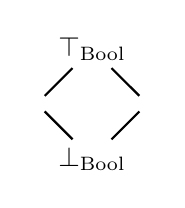
\begin{tikzpicture}
    \node (top) at (0,0) {$\top_{\mbox{\scriptsize Bool}}$};
    \node (midleft) at (-0.7,-0.7) {$\atrue$};
    \node (midright) at (0.7,-0.7) {$\afalse$};
    \node (down) at (0,-1.4) {$\bot_{\mbox{\scriptsize Bool}}$};
    \draw [black, thick, shorten <= -1pt, shorten >=-1pt] (top) -- (midleft);
    \draw [black, thick, shorten <= -1pt, shorten >=-1pt] (top) -- (midright);
    \draw [black, thick, shorten <= -1pt, shorten >=-1pt] (midleft) -- (down);
    \draw [black, thick, shorten <= -1pt, shorten >=-1pt] (midright) -- (down);
  \end{tikzpicture}
\end{matrix}
\quad
\abs{Absent} =
\begin{matrix}
  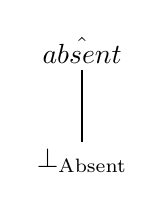
\begin{tikzpicture}
    \node (top) at (0,0) {$\hat{\SF{absent}}$};
    \node (down) at (0,-1.4) {$\bot_{\mbox{\scriptsize Absent}}$};
    \draw [black, thick, shorten <= -1pt, shorten >=-1pt] (top) -- (down);
  \end{tikzpicture}
\end{matrix}
\]
\[
\abs{Number} = 
\begin{matrix} 
  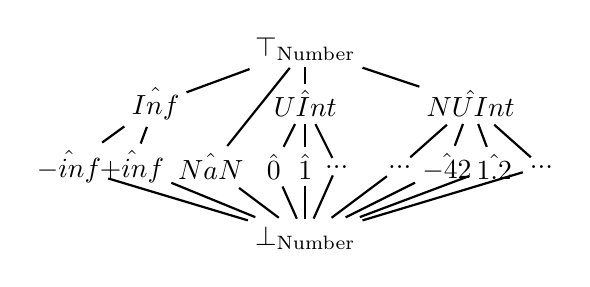
\begin{tikzpicture}
    % First, locate each of the nodes and name them
    \node (top) at (0,0) {$\top_{\mbox{\scriptsize Number}}$};
    \node (upperleft) at (-1.9,-0.7) {$\hat{\SF{Inf}}$};
    \node (uppercenter) at (0,-0.7) {$\hat{\SF{UInt}}$};
    \node (upperright) at (2.1,-0.7) {$\hat{\SF{NUInt}}$};
    \node (lower1) at (-3.0,-1.5) {$\hat{\SF{-inf}}$};
    \node (lower2) at (-2.2,-1.5) {$\hat{\SF{+inf}}$};
    \node (lower3) at (-1.2,-1.5) {$\hat{\SF{NaN}}$};
    \node (lower4) at (-0.4,-1.5) {$\hat{0}$};
    \node (lower5) at (0,-1.5) {$\hat{1}$};
    \node (lower6) at (0.4,-1.5) {...};
    \node (lower7) at (1.2,-1.5) {...};
    \node (lower8) at (1.8,-1.5) {$\hat{-42}$};
    \node (lower9) at (2.4,-1.5) {$\hat{1.2}$};
    \node (lower10) at (3,-1.5) {...};
    \node (down) at (0,-2.4) {$\bot_{\mbox{\scriptsize Number}}$};
    % Now draw the lines0
    \draw [black, thick, shorten <= -1pt, shorten >=-1pt] (top) -- (upperleft);
    \draw [black, thick, shorten <= -1pt, shorten >=-1pt] (top) -- (uppercenter);
    \draw [black, thick, shorten <= -1pt, shorten >=-1pt] (top) -- (upperright);
    \draw [black, thick, shorten <= -1pt, shorten >=-1pt] (top) -- (lower3);
    \draw [black, thick, shorten <= -1pt, shorten >=-1pt] (upperleft) -- (lower1);
    \draw [black, thick, shorten <= -1pt, shorten >=-1pt] (upperleft) -- (lower2);
    \draw [black, thick, shorten <= -1pt, shorten >=-1pt] (uppercenter) -- (lower4);
    \draw [black, thick, shorten <= -1pt, shorten >=-1pt] (uppercenter) -- (lower5);
    \draw [black, thick, shorten <= -1pt, shorten >=-1pt] (uppercenter) -- (lower6);
    \draw [black, thick, shorten <= -1pt, shorten >=-1pt] (upperright) -- (lower7);
    \draw [black, thick, shorten <= -1pt, shorten >=-1pt] (upperright) -- (lower8);
    \draw [black, thick, shorten <= -1pt, shorten >=-1pt] (upperright) -- (lower9);
    \draw [black, thick, shorten <= -1pt, shorten >=-1pt] (upperright) -- (lower10);
    \draw [black, thick, shorten <= -1pt, shorten >=-1pt] (lower1) -- (down);
    \draw [black, thick, shorten <= -1pt, shorten >=-1pt] (lower2) -- (down);
    \draw [black, thick, shorten <= -1pt, shorten >=-1pt] (lower3) -- (down);
    \draw [black, thick, shorten <= -1pt, shorten >=-1pt] (lower4) -- (down);
    \draw [black, thick, shorten <= -1pt, shorten >=-1pt] (lower5) -- (down);
    \draw [black, thick, shorten <= -1pt, shorten >=-1pt] (lower6) -- (down);
    \draw [black, thick, shorten <= -1pt, shorten >=-1pt] (lower7) -- (down);
    \draw [black, thick, shorten <= -1pt, shorten >=-1pt] (lower8) -- (down);
    \draw [black, thick, shorten <= -1pt, shorten >=-1pt] (lower9) -- (down);
    \draw [black, thick, shorten <= -1pt, shorten >=-1pt] (lower10) -- (down);
  \end{tikzpicture}
\end{matrix}
\]
\[
\abs{String} = 
	\begin{matrix} 
		\begin{tikzpicture}
	    % First, locate each of the nodes and name them
	    \node (top) at (0,0) {$\top_{\mbox{\scriptsize String}}$};
	    \node (upperleft) at (-1,-0.7) {$\hat{\SF{NumStr}}$};
	    \node (upperright) at (1,-0.7) {$\hat{\SF{OtherStr}}$};
	    \node (lower1) at (-2,-1.5) {$\hat{``\SF{NaN}"}$};
	    \node (lower2) at (-1.2,-1.5) {$\hat{``1.1"}$};
	    \node (lower3) at (-0.4,-1.5) {...};
	    \node (lower4) at (0.4,-1.5) {$\hat{``\mbox{foo}"}$};
	    \node (lower5) at (1.5,-1.5) {$\hat{``\mbox{bar}"}$};
	   	\node (lower6) at (2.2,-1.5) {...};
	    \node (down) at (0,-2.4) {$\bot_{\mbox{\scriptsize String}}$};
	    % Now draw the lines0
	  	\draw [black, thick, shorten <= -1pt, shorten >=-1pt] (top) -- (upperleft);
	  	\draw [black, thick, shorten <= -1pt, shorten >=-1pt] (top) -- (upperright);
	  	\draw [black, thick, shorten <= -1pt, shorten >=-1pt] (midleft) -- (lower1);
	  	\draw [black, thick, shorten <= -1pt, shorten >=-1pt] (midleft) -- (lower2);
	  	\draw [black, thick, shorten <= -1pt, shorten >=-1pt] (midleft) -- (lower3);
	  	\draw [black, thick, shorten <= -1pt, shorten >=-1pt] (midright) -- (lower4);
	  	\draw [black, thick, shorten <= -1pt, shorten >=-1pt] (midright) -- (lower5);
	  	\draw [black, thick, shorten <= -1pt, shorten >=-1pt] (midright) -- (lower6);
	  	\draw [black, thick, shorten <= -1pt, shorten >=-1pt] (lower1) -- (down);
	  	\draw [black, thick, shorten <= -1pt, shorten >=-1pt] (lower2) -- (down);
	  	\draw [black, thick, shorten <= -1pt, shorten >=-1pt] (lower3) -- (down);
	  	\draw [black, thick, shorten <= -1pt, shorten >=-1pt] (lower4) -- (down);
	  	\draw [black, thick, shorten <= -1pt, shorten >=-1pt] (lower5) -- (down);
	  	\draw [black, thick, shorten <= -1pt, shorten >=-1pt] (lower6) -- (down);
		\end{tikzpicture}
	\end{matrix}
\]

\newpage
\section{Domain Operators}
\subsection{Heap}
\subsection{Context}
\subsection{Obj}

\newpage
\section{Context-sensitivity}
\subsection{Context-insensitive}
\subsection{k-callsite-sensitive}

\newpage
\section{Helper Functions}

\subsection{Prunning Helper Functions}

\newpage
\section{Semantics}
\[
\begin{array}{lcl}
\aE & \in & \abs{IPEdge} \rightarrow \aState \rightarrow \aState \\
\aC & \in & \aControlPoint \rightarrow \aState \rightarrow \aState \times \aState\\
\aI & \in & \SF{Instruction} 
    \rightarrow \aState \times \aState \rightarrow \aState \times \aState\\
\aCI & \in & \aControlPoint \rightarrow \SF{CallInstruction} 
    \rightarrow \aState \times \aState \rightarrow \aState \times \aState\\
\aV & \in & \SF{Expression} \rightarrow \aState 
    \rightarrow \aValue \times \powerset{\abs{Exception}} \\
\aB & \in & \SF{Expression} \rightarrow \aState \times \aState 
    \rightarrow \aState \times \aState\\
\end{array}
\]

\subsection{Interprocedural Edge}
\[
\renewcommand\arraystretch{1.5}
\begin{array}{l}
% call edge (bottom heap)
\aE \lbr ( \acp, (n \in \SF{Entry},\hat{cc}), \hat{C}, \hat{o} ) \rbr (\bot_{Heap},\hat{C}_1) 
    = \bot_{State}\\

% call edge
\aE \lbr ( \acp, (n \in \SF{Entry},\hat{cc}), \hat{C},\hat{o} ) \rbr (\hat{H}_1,\hat{C}_1) 
    = (\hat{H}_3,\hat{C}_1) \\
  \quad\wherec{
    \hat{H}_3 = \bigsqcup_{\hat{l}_{env}\in \hat{L}_{env}} \hat{H}_2[\hat{l}_{env} \mapsto \hat{o}_{env}]\\
    \land\ \hat{L}_{env} = \hat{o}_2(\varprop{env})\emph{.objval.value.locSet}\\
    \land\ \hat{H}_2 = \hat{H}_1[\avarloc{PureLocal}_R \mapsto \hat{o}_2] \\
    \land\ \hat{o}_2 = \hat{o} - \varprop{scope} \\
    \land\ \hat{o}_{env} = \ahf{NewDeclEnvRecord}(\hat{v}) \\
    \land\ \hat{v} = \hat{o}(\varprop{scope})\emph{.objval.value}
  }
\\\\

% normal return edge (bottom heap/context)
\aE \lbr ( (n \in \SF{Exit}, \hat{cc}), \acp, \hat{C},\hat{o} ) \rbr (\bot_{Heap}, \hat{C}_1)
    = \bot_{State}\\

\aE \lbr ( (n \in \SF{Exit}, \hat{cc}), \acp, \hat{C},\hat{o} ) \rbr (\hat{H}_1, \bot_{Context})
    = \bot_{State}\\

% normal return edge
\aE \lbr ( (n_1 \in \SF{Exit}, \hat{cc}_1), (n_2 \in \SF{AfterCall}, \hat{cc}_2), \hat{C}, \hat{o} ) \rbr (\hat{H}_1, \hat{C}_1)
   = \left\{
   \begin{array}{ll}
   \emph{\TT{new}\ State}(\hat{H}_3, \hat{C}_2) & \ifc{\hat{C}_2 \neq \bot_{Context}}\\
   \bot_{State} & \ifc{\hat{C}_2 = \bot_{Context}}\\
   \end{array}
   \right. \\
\quad\wherec{
    \hat{H}_3 = \ahf{VarStore}(\hat{H}_2, n_2\emph{.retVar}, \hat{v})\\
	\land\ \hat{H}_2 = \hat{H}_1[\avarloc{PureLocal} \mapsto \hat{o}_1]\\
	\land\ \hat{v} = \hat{H}_1(\avarloc{PureLocal})\\
	\land\ (\hat{C}_2, \hat{o}_1) = \ahf{FixOldify}(\hat{C},\ \hat{o},\ \hat{C}_1\emph{.mayOld},\ \hat{C}_1\emph{.mustOld})
}\\\\

\aE \lbr ( (n_1 \in \SF{Exit}, \hat{cc}_1), (n_2 \not\in \SF{AfterCall}, \hat{cc}_2), \hat{C}, \hat{o} ) \rbr\ \hat{S}
    \quad \comment{\inblue Impossible Case: IPFromExitToNoneError} \\

% exception return edge (bottom heap/context)
\aE \lbr ( (n \in \SF{ExitExc}, \hat{cc}), \acp, \hat{C},\hat{o} ) \rbr (\bot_{Heap}, \hat{C}_1)
    = \bot_{State}\\

\aE \lbr ( (n \in \SF{ExitExc}, \hat{cc}), \acp, \hat{C},\hat{o} ) \rbr (\hat{H}_1, \bot_{Context})
    = \bot_{State}\\

% exception return inter-procedural edge
\aE \lbr ( (n_1 \in \SF{ExitExc}, \hat{cc}_1), (n_2 \in \SF{AfterCatch}, \hat{cc}_2), \hat{C}, \hat{o} ) \rbr (\hat{H}_1, \hat{C}_1)
   = \left\{
   \begin{array}{ll}
   \emph{\TT{new}\ State}(\hat{H}_2, \hat{C}_2) & \ifc{\hat{C}_2 \neq \bot_{Context}}\\
   \bot_{State} & \ifc{\hat{C}_2 = \bot_{Context}}\\
   \end{array}
   \right. \\
\quad\wherec{
    \hat{H}_2 = \hat{H}_1 \left[ \avarloc{PureLocal} \mapsto 
        \hat{o}_1 \left[ \begin{array}{ll}
		    \varprop{exception} \mapsto \hat{v}_1, \\
			\varprop{exception\_all} \mapsto \hat{v}_1 \sqcup \hat{v}_2
		\end{array} \right] \right] \\
	\land\ \hat{v}_1 = \hat{H}_1(\avarloc{PureLocal})(\varprop{exception})\emph{.objval.value}\\
	\land\ \hat{v}_2 = \hat{o}_1(\varprop{exception\_all})\emph{.objval.value}\\
	\land\ (\hat{C}_2, \hat{o}_1) = \ahf{FixOldify}(\hat{C},\ \hat{o},\ \hat{C}_1\emph{.mayOld},\ \hat{C}_1\emph{.mustOld})
}\\\\

\aE \lbr ( (n_1 \in \SF{ExitExc}, \hat{cc}_1), (n_2 \not\in \SF{AfterCatch}, \hat{cc}_2), \hat{C}, \hat{o} ) \rbr\ \hat{S}
    \quad \comment{\inblue Impossible Case: IPFromExitToNoneError} \\

\end{array}
\]

\subsection{Block}
\[
\renewcommand\arraystretch{1.5}
\begin{array}{l}

\aC \lbr \hat{cp} \rbr\ \bot_{State} = (\bot_{State}, \bot_{State}) \\

% Entry Block
\aC \lbr (n \in \SF{Entry}, \hat{cc}) \rbr (\hat{H}_0, \hat{C}) = ((\hat{H}_m, \hat{C}), \bot_{State}) \\
\quad\wherec{
\forall n+1 \leq j \leq m.\ \hat{H}_j = \ahf{CreateMutableBinding}(\hat{H}_{j-1}, x_j, \abs{Value}(\aundef)) \\
\land\ \forall 1 \leq i \leq n.\ \hat{H}_i = \ahf{CreateMutableBinding}(\hat{H}_{i-1}, x_i,
    \bigsqcup_{\hat{l}_{arg} \in \hat{L}_{arg}}\ \ahf{Proto}(\hat{H}_{i-1}, \hat{l}_{arg}, \hat{``i-1"}) \\
\land\ x_{n+1} \cdots x_m = n\emph{.func.localVars} \
\land\ x_1 \cdots x_n = n\emph{.func.argVars} \\
\land\ \hat{L}_{arg} = \hat{H}_0(\avarloc{PureLocal})(n\emph{.func.argumentsName})\emph{.objval.value.locSet}
}\\\\

% Exit Block
\aC \lbr (n \in \SF{Exit}, \hat{cc}) \rbr\ \hat{S} = (\hat{S}, \bot_{State}) \\

% ExitExc Block
\aC \lbr (n \in \SF{ExitExc}, \hat{cc}) \rbr\ \hat{S} = (\hat{S}, \bot_{State}) \\

% Call Block
\aC \lbr (n \in \SF{Call}, \hat{cc}) \rbr\ \hat{S} 
= \aCI_{(n, \hat{cc})} \lbr n\emph{.callInst} \rbr (\hat{S}, \bot_{State}) \\

% AfterCall Block
\aC \lbr (n \in \SF{AfterCall}, \hat{cc}) \rbr\ \hat{S} = (\hat{S}, \bot_{State}) \\

% AfterCatch Block
\aC \lbr (n \in \SF{AfterCatch}, \hat{cc}) \rbr\ \hat{S} = (\hat{S}, \bot_{State}) \\

% Normal Block
\aC \lbr (n \in \SF{Block}, \hat{cc}) \rbr\ \hat{S}_0 = (\hat{S}_n, \hat{E}_n) \\
\quad\wherec{
\forall 1 \leq k \leq n.\ 
(\hat{S}_k, \hat{E}_k) = \aI \lbr i_k \rbr (\hat{S}_{k-1}, \hat{E}_{k-1}) \\
\land\ i_1 \cdots i_n = n\emph{.insts} \
\land\ \hat{E}_0 = \bot_{State}
}\\\\

\end{array}
\]

\subsection{Instruction}
\[
\renewcommand\arraystretch{1.5}
\begin{array}{l}

\aI \lbr i \rbr ((\bot_{Heap}, \hat{C}), \hat{S})  = (\bot_{State}, \hat{S}) \\\\

% CFGAlloc
\aI \lbr x~\verb+:=+~\TT{alloc}\verb+(+ \verb+)+_{\hat{a}} \rbr\ (\hat{S}, \hat{E}) = ((\hat{H}_3, \hat{C}_1), \hat{E}) \\
\quad\wherec{
\hat{H}_3 = \ahf{VarStore}(\hat{H}_2, x, \abs{Value}(\hat{l}_R)) \\
\land\ \hat{H}_2 = \ahf{AllocObject}(\hat{H}_1, \hat{L}_v, \hat{l}_R) \\
\land\ (\hat{H}_1, \hat{C}_1) = \ahf{Oldify}(\hat{S}, \hat{a}) \
\land\ \hat{l}_R = \emph{\TT{new} Loc}(\hat{a}, \hat{Recent}) \\
\land\ \hat{L}_v = \{\avarloc{ObjProto}\}
}\\\\

\aI \lbr x~\verb+:=+~\TT{alloc}\verb+(+ e \verb+)+_{\hat{a}} \rbr\ (\hat{S}, \hat{E}) = ((\hat{H}_3, \hat{C}_1), \hat{E}_1) \\
\quad\wherec{
\hat{H}_3 = \ahf{VarStore}(\hat{H}_2, x, \abs{Value}(\hat{l}_R)) \\
\land\ \hat{H}_2 = \ahf{AllocObject}(\hat{H}_1, \hat{L}_v, \hat{l}_R) \\
\land\ (\hat{H}_1, \hat{C}_1) = \ahf{Oldify}(\hat{S}, \hat{a}) \
\land\ \hat{l}_R = \emph{\TT{new} Loc}(\hat{a}, \hat{Recent}) \\
\land\ \hat{L}_v = 
    \left \{ \begin{array}{ll} 
	\hat{v}\emph{.locSet} & \ifc{\hat{v}\emph{.pvalue} \not\sqsubseteq \bot_{PValue}}\\
	\hat{v}\emph{.locSet}\ \cup\ \{\avarloc{ObjProto}\} & \owc \\
	\end{array} \right.\\
\land\ \hat{E}_1 = \hat{E} + \ahf{RaiseException}(\hat{S}, \hat{es}) \\
\land\ (\hat{v}, \hat{es}) = \aV \lbr e \rbr\ (\hat{H}_1, \hat{C}_1)
}\\\\

\end{array}
\]

\[
\renewcommand\arraystretch{1.5}
\begin{array}{l}


% CFGAllocArray
\aI \lbr x~\verb+:=+~\TT{allocArray}\verb+(+n\verb+)+_{\hat{a}} \rbr\ (\hat{S}, \hat{E}) = ((\hat{H}_3, \hat{C}_1), \hat{E}) \\
\quad\wherec{
\hat{H}_3 = \ahf{VarStore}(\hat{H}_2, x, \abs{Value}(\hat{l}_R)) \\
\land\ \hat{H}_2 = \hat{H}_1 [\hat{l}_R \mapsto \ahf{NewArrayObject}(\hat{n})] \\
\land\ (\hat{H}_1, \hat{C}_1) = \ahf{Oldify}(\hat{S}, \hat{a}) \
\land\ \hat{l}_R = \emph{\TT{new} Loc}(\hat{a}, \hat{Recent}) \\
\land\ \hat{n} = \hat{v}\emph{.pvalue.numVal} \
\land\ (\hat{v}, -) = \aV \lbr e \rbr\ (\hat{H}_1, \hat{C}_1)
}\\\\

% CFGAllocArg
\aI \lbr x~\verb+:=+~\TT{allocArg}\verb+(+n\verb+)+_{\hat{a}} \rbr\ (\hat{S}, \hat{E}) = ((\hat{H}_3, \hat{C}_1), \hat{E}) \\
\quad\wherec{
\hat{H}_3 = \ahf{VarStore}(\hat{H}_2, x, \abs{Value}(\hat{l}_R)) \\
\land\ \hat{H}_2 = \hat{H}_1 [\hat{l}_R \mapsto \ahf{NewArgObject}(\hat{n})] \\
\land\ (\hat{H}_1, \hat{C}_1) = \ahf{Oldify}(\hat{S}, \hat{a}) \
\land\ \hat{l}_R = \emph{\TT{new} Loc}(\hat{a}, \hat{Recent}) \\
\land\ \hat{n} = \hat{v}\emph{.pvalue.numVal} \
\land\ (\hat{v}, -) = \aV \lbr e \rbr\ (\hat{H}_1, \hat{C}_1)
}\\\\

% CFGExprStmt
\aI \lbr x ~\verb+:=+~ e \rbr\ ((\hat{H}, \hat{C}), \hat{E}) = ((\hat{H}_1, \hat{C}_1), \hat{E}_1) \\
\quad\wherec{
(\hat{H}_1, \hat{C}_1) = \left \{ \begin{array}{ll}
(\ahf{VarStore}(\hat{H}, x, \hat{v}),\ \hat{C}) & \ifc{\hat{v} \not\sqsubseteq \bot_{Value}}\\
(\bot_{Heap}, \bot_{Context}) & \owc \\
\end{array} \right.\\
\land\ \hat{E}_1 = \hat{E} \sqcup \ahf{RaiseException}((\hat{H}, \hat{C}),\ \hat{es}) \\
\land\ (\hat{v}, \hat{es}) = \aV \lbr e \rbr (\hat{H}, \hat{C})
}\\\\

% CFGDelete
\aI \lbr x_1 ~\verb+:=+~ \TT{delete}\verb+(+x_2\verb+)+ \rbr\ ((\hat{H}, \hat{C}), \hat{E}) = ((\hat{H}_2, \hat{C}), \hat{E}) \\
\quad\wherec{
\hat{H}_2 = \ahf{VarStore}(\hat{H}_1,\ x_1,\ \abs{Value}(\hat{b})) \\
\land\ (\hat{H}_1, \hat{b}) = \left \{ \begin{array}{ll}
(\hat{H}, \atrue) & \ifc{\hat{L}_{base} = \varnothing} \\
\bigsqcup_{\hat{l} \in \hat{L}_{base}} \ahf{Delete}(\hat{H},\ \hat{l},\ \hat{x_2}) & \owc \\
\end{array} \right. \\
\land\ \hat{L}_{base} = \ahf{LookupBase}(\hat{H},\ x_2)
}\\\\

\aI \lbr x ~\verb+:=+~ \TT{delete}\verb+(+e\verb+)+ \rbr\ ((\hat{H}, \hat{C}), \hat{E}) = ((\hat{H}_1, \hat{C}_1), \hat{E}_1) \\
\quad\wherec{
(\hat{H}_1, \hat{C}_1) = \left \{ \begin{array}{ll}
(\ahf{VarStore}(\hat{H},\ x,\ \abs{Value}(\atrue),\ \hat{C}) & \ifc{ \hat{v} \not\sqsubseteq \bot_{Value}} \\
(\bot_{Heap},\ \bot_{Context}) & \owc \\
\end{array} \right.\\
\land\ \hat{E}_1 = \hat{E} \sqcup \ahf{RaiseException}((\hat{H}, \hat{C}), \hat{es}) \\
\land\ (\hat{v}, \hat{es}) = \aV \lbr e \rbr (\hat{H}, \hat{C})
}\\\\

% CFGDeleteProp
\aI \lbr x ~\verb+:=+~ \TT{delete}\verb+(+e_1,e_2\verb+)+ \rbr\ ((\hat{H}, \hat{C}), \hat{E}) = ((\hat{H}_2, \hat{C}_2), \hat{E}_1) \\
\quad\wherec{
(\hat{H}_2, \hat{C}_2) = \left \{ \begin{array}{ll}
(\ahf{VarStore}(\hat{H}_1,\ x,\ \abs{Value}(\hat{b})),\ \hat{C}) & \ifc{\hat{H}_1 \not\sqsubseteq \bot_{Heap}} \\
(\bot_{Heap}, \bot_{Context}) & \owc \\
\end{array} \right.\\
\land\ (\hat{H}_1, \hat{b}) = \left \{ \begin{array}{ll}
\bigsqcup_{\hat{l} \in \hat{v}_1\emph{.locSet}} \bigsqcup_{\hat{s} \in S_{idx}} \ahf{Delete}(\hat{H},\ \hat{l},\ \hat{s}) 
    & \ifc{\hat{v}_1\emph{.locSet} \neq \varnothing \land\ S_{idx} \neq \varnothing} \\
(\bot_{Heap}, \bot_{Bool}) & \owc \\
\end{array} \right. \\
\land\ \hat{E}_1 = \hat{E} \sqcup \ahf{RaiseException}((\hat{H}, \hat{C}), \hat{es}) \\
\land\ S_{idx} = \left \{ \begin{array}{ll}
\ahf{toStringSet}(\ahf{toPrimitiveBetter}(\hat{H}, \hat{v}_2)) & \ifc{\hat{v}_2 \not\sqsubseteq \bot_{Value}} \\
\varnothing & \owc \\
\end{array} \right.\\
\land\ (\hat{v}_1, -) = \aV \lbr e_1 \rbr (\hat{H}, \hat{C}) \
\land\ (\hat{v}_2, \hat{es}) = \aV \lbr e_2 \rbr (\hat{H}, \hat{C})
}\\\\

\end{array}
\]

\[
\renewcommand\arraystretch{1.5}
\begin{array}{l}

% CFGStoreStringIdx
\aI \lbr e_1 \verb+[+s\verb+]+ ~\verb+:=+~ e_3 \rbr\ ((\hat{H}, \hat{C}), \hat{E})
= \left \{ \begin{array}{ll}
((\bot_{Heap}, \hat{C}),\ \hat{E} \sqcup \hat{E}_1) & \ifc{ \hat{v}_3 \sqsubseteq \bot_{Value} } \\
((\hat{H}_1, \hat{C}),\ \hat{E} \sqcup \hat{E}_2) & \owc \\
\end{array} \right. \\
\quad\wherec{
\hat{E}_1 = \ahf{RaiseException}((\hat{H}, \hat{C}),\ \hat{es}_3) \\
\land\ \hat{E}_2 = \ahf{RaiseException}((\hat{H}, \hat{C}),\ \hat{es}_3 \sqcup \hat{es}_4) \\

\land\ \hat{H}_1 = \hat{H}_{cantPut} \sqcup \hat{H}_{notArr} \sqcup \hat{H}_{Arr} \\
\land\ \hat{H}_{cantPut} = \left \{ \begin{array}{ll} 
\hat{H} & \ifc{\exists\ \hat{l} \in \hat{L}_1 ~\mid~ \afalse \sqsubseteq \ahf{CanPut}(\hat{H},\ \hat{l},\ \hat{s}) } \\
\bot_{Heap} & \owc \\
\end{array} \right.\\

\land\ \hat{H}_{notArr} = \bigsqcup_{\hat{l}_n \in \hat{L}_{notArr}} \ahf{PropStore}(\hat{H},\ \hat{l}_n,\ \hat{s},\ \hat{v}_3) \\

\land\ (\hat{H}_{Arr},\ \hat{es}_4) = \bigsqcup_{\hat{l}_a \in \hat{L}_{Arr}} 
(\hat{H}_{length} \sqcup \hat{H}_{idx} \sqcup \hat{H}_{other},\ \hat{es}_{length}) \\
\quad\wherec {
(\hat{H}_{length},\ \hat{es}_{length}) = \ahf{ArrayLenghtStore}(\hat{H},\ \hat{s},\ \hat{v},\ \hat{l}_a) \\
\land\ \hat{H}_{idx} = \ahf{ArrayIdxStore}(\hat{H},\ \hat{s},\ \hat{v},\ \hat{l}_a) \\
\land\ \hat{H}_{other} = \left \{ \begin{array}{ll}
\ahf{PropStore}(\hat{H},\ \hat{l}_a,\ \hat{s},\ \hat{v}_3) 
& \ifc{\hat{s} \hat{\neq} \hat{``length"}\ \land\ \afalse \sqsubseteq \hat{s}\emph{.isArrayIndex} } \\
\bot_{Heap} & \owc
\end{array} \right.
} \vspace{1mm} \\

\land\ \hat{L}_{notArr} = \set{\hat{l} \in \hat{L}_1 ~\mid~  \afalse \sqsubseteq \ahf{IsArray}(\hat{H},\ \hat{l}) \ 
\land\ \atrue \sqsubseteq \ahf{CanPut}(\hat{H},\ \hat{l},\ \hat{s}) } \\
\land\ \hat{L}_{Arr} = \set{\hat{l} \in \hat{L}_1 ~\mid~  \atrue \sqsubseteq \ahf{IsArray}(\hat{H},\ \hat{l}) \ 
\land\ \atrue \sqsubseteq \ahf{CanPut}(\hat{H},\ \hat{l},\ \hat{s}) } \\
\land\ \hat{L}_1 = \hat{v}_1\emph{.locSet} \
\land\ (\hat{v}_1, \hat{es}_1) = \aV \lbr e_1 \rbr (\hat{H}, \hat{C}) \
\land\ (\hat{v}_3, \hat{es}_3) = \aV \lbr e_3 \rbr (\hat{H}, \hat{C})
} \\\\

% CFGStore
\aI \lbr e_1 \verb+[+ e_2 \verb+]+ ~\verb+:=+~ e_3 \rbr\ ((\hat{H}, \hat{C}), \hat{E})
= \left \{ \begin{array}{ll}
((\bot_{Heap}, \hat{C}),\ \hat{E} \sqcup \hat{E}_1) & \ifc{ \hat{v}_3 \sqsubseteq \bot_{Value} } \\
((\hat{H}_1, \hat{C}),\ \hat{E} \sqcup \hat{E}_2) & \owc \\
\end{array} \right. \\
\quad\wherec{
\hat{E}_1 = \ahf{RaiseException}((\hat{H}, \hat{C}),\ \hat{es}_2 \sqcup \hat{es}_3) \\
\land\ \hat{E}_2 = \ahf{RaiseException}((\hat{H}, \hat{C}),\ \hat{es}_2 \sqcup \hat{es}_3 \sqcup \hat{es}_4) \\

\land\ (\hat{H}_1,\ \hat{es}_4) = \bigsqcup_{\hat{s} \in S_{idx}}
(\hat{H}_{cantPut} \sqcup \hat{H}_{notArr} \sqcup \hat{H}_{Arr},\ \hat{es}_{Arr}) \\
\quad\wherec{
\hat{H}_{cantPut} = \left \{ \begin{array}{ll} 
\hat{H} & \ifc{\exists\ \hat{l} \in \hat{L}_1 ~\mid~ \afalse \sqsubseteq \ahf{CanPut}(\hat{H},\ \hat{l},\ \hat{s}) } \\
\bot_{Heap} & \owc \\
\end{array} \right.\\

\land\ \hat{H}_{notArr} = \bigsqcup_{\hat{l}_n \in \hat{L}_{notArr}} \ahf{PropStore}(\hat{H},\ \hat{l}_n,\ \hat{s},\ \hat{v}_3) \\

\land\ (\hat{H}_{Arr},\ \hat{es}_{Arr}) = \bigsqcup_{\hat{l}_a \in \hat{L}_{Arr}} 
(\hat{H}_{length} \sqcup \hat{H}_{idx} \sqcup \hat{H}_{other},\ \hat{es}_{length}) \\
\quad\wherec {
(\hat{H}_{length},\ \hat{es}_{length}) = \ahf{ArrayLenghtStore}(\hat{H},\ \hat{s},\ \hat{v},\ \hat{l}_a) \\
\land\ \hat{H}_{idx} = \ahf{ArrayIdxStore}(\hat{H},\ \hat{s},\ \hat{v},\ \hat{l}_a) \\
\land\ \hat{H}_{other} = \left \{ \begin{array}{ll}
\ahf{PropStore}(\hat{H},\ \hat{l}_a,\ \hat{s},\ \hat{v}_3) 
& \ifc{\hat{s} \hat{\neq} \hat{``length"}\ \land\ \afalse \sqsubseteq \hat{s}\emph{.isArrayIndex} } \\
\bot_{Heap} & \owc
\end{array} \right.
} \vspace{1mm} \\

\land\ \hat{L}_{notArr} = \set{\hat{l} \in \hat{L}_1 ~\mid~  \afalse \sqsubseteq \ahf{IsArray}(\hat{H},\ \hat{l}) \ 
\land\ \atrue \sqsubseteq \ahf{CanPut}(\hat{H},\ \hat{l},\ \hat{s}) } \\
\land\ \hat{L}_{Arr} = \set{\hat{l} \in \hat{L}_1 ~\mid~  \atrue \sqsubseteq \ahf{IsArray}(\hat{H},\ \hat{l}) \ 
\land\ \atrue \sqsubseteq \ahf{CanPut}(\hat{H},\ \hat{l},\ \hat{s}) } \\
} \vspace{1mm} \\

\land\ \hat{L}_1 = \hat{v}_1\emph{.locSet} \
\land\ S_{idx} = \hat{v}_2\emph{.toPrimitive.toStringSet} \\
\land\ (\hat{v}_1, \hat{es}_1) = \aV \lbr e_1 \rbr (\hat{H}, \hat{C}) \
\land\ (\hat{v}_2, \hat{es}_2) = \aV \lbr e_2 \rbr (\hat{H}, \hat{C}) \
\land\ (\hat{v}_3, \hat{es}_3) = \aV \lbr e_3 \rbr (\hat{H}, \hat{C})
} \\\\

\end{array}
\]

\[
\renewcommand\arraystretch{1.5}
\begin{array}{l}

% CFGFunExpr
\aI \lbr x ~\verb+:=+~ \TT{function} ~\verb+(+f\verb+)+_{\hat{a}_1, \hat{a}_2} \rbr\ (\hat{S}, \hat{E}) 
= ((\hat{H}_5, \hat{C}_2), \hat{E}) \\
\quad\wherec{
\hat{H}_5 = \ahf{VarStore}(\hat{H}_4,\ x,\ \abs{Value}(\hat{l}_{R1})) \\
\land\ \hat{H}_4 = \hat{H}_3 \left[\hat{l}_{R2} \mapsto \hat{o}_{new}
\left[``constructor" \mapsto \langle \abs{Value}(\hat{l}_{R1}),\ \atrue,\ \afalse,\ \atrue \rangle \right]
\right] \\
\land\ \hat{H}_3 = \hat{H}_2 
\left[\hat{l}_{R1} \mapsto \ahf{NewFunctionObject}(fid,\ \hat{v}_{env},\ \hat{l}_{R2},\ \hat{n}) \right] \\
\land\ (\hat{H}_2, \hat{C}_2) = \ahf{Oldify}(\hat{S}_1, \hat{a}_2) \
\land\ \hat{S}_1 = \ahf{Oldify}(\hat{S}, \hat{a}_1) \\
\land\ \hat{l}_{R1} = \emph{\TT{new} Loc}(\hat{a}_1, \hat{Recent}) \
\land\ \hat{l}_{R2} = \emph{\TT{new} Loc}(\hat{a}_2, \hat{Recent}) \\
\land\ \hat{o}_{new} = \ahf{NewObject}(\avarloc{ObjectProto})\\
\land\ \hat{v}_{env} = \hat{H}_2(\avarloc{PureLocal})(\varprop{env})\emph{.objval.value} \\
\land\ \hat{n} = f\emph{.argVars.length} \\
}\\\\

\aI \lbr x_1 ~\verb+:=+~ \TT{function} ~x_2 \verb+(+f\verb+)+_{\hat{a}_1,\ \hat{a}_2,\ \hat{a}_3} \rbr\ (\hat{S}, \hat{E}) = ((\hat{H}_7, \hat{C}_3), \hat{E}) \\
\quad\wherec{
\land\ \hat{H}_7 = \ahf{VarStore}(\hat{H}_6, x_1, \abs{Value}(\hat{l}_{R1})) \\
\land\ \hat{H}_6 = \hat{H}_5 \left[ \hat{l}_{R3} \mapsto \hat{o}_{env}
\left[ x_2 \mapsto \langle \abs{Value}(\hat{l}_{R1}),\ \afalse,\ \bot_{Bool},\ \afalse \rangle \right]
\right] \\
\land\ \hat{H}_5 = \hat{H}_4 \left[ \hat{l}_{R2} \mapsto \hat{o}_{new} 
\left[ ``constructor" \mapsto \langle \abs{Value}(\hat{l}_{R1}),\ \atrue,\ \afalse,\ \atrue \rangle \right]
\right] \\
\land\ \hat{H}_4 = \hat{H}_3 
\left[ \hat{l}_{R1} \mapsto \ahf{NewFunctionObject}(fid,\ \abs{Value}(\hat{l}_{R3}),\ \hat{l}_{R2},\ \hat{n})) \right] \\
\land\ (\hat{H}_3, \hat{C}_3) = \ahf{Oldify}(\hat{S}_2, \hat{a}_3) \
\land\ \hat{S}_2 = \ahf{Oldify}(\hat{S}_1, \hat{a}_2) \
\land\ \hat{S}_1 = \ahf{Oldify}(\hat{S}, \hat{a}_1) \\
\land\ \hat{l}_{R1} = \emph{\TT{new} Loc}(\hat{a}_1, \hat{Recent}) \
\land\ \hat{l}_{R2} = \emph{\TT{new} Loc}(\hat{a}_2, \hat{Recent}) \
\land\ \hat{l}_{R3} = \emph{\TT{new} Loc}(\hat{a}_3, \hat{Recent}) \\
\land\ \hat{o}_{env} = \ahf{NewDeclEnvRecord}(\hat{v}_{env}) \
\land\ \hat{o}_{new} = \ahf{NewObject}(\avarloc{ObjectProto}) \\
\land\ \hat{v}_{env} = \hat{H}_3(\avarloc{PureLocal})(\varprop{env})\emph{.objval.value} \\
\land\ \hat{n} = f\emph{.argVars.length} \\
}\\\\

% CFGReturn
\aI \lbr \TT{return} \rbr\ ((\hat{H}, \hat{C}), \hat{E}) = ((\hat{H}_1, \hat{C}), \hat{E}) \\
\quad\wherec{
\hat{H}_1 = \hat{H} \left[ \avarloc{PureLocal} \mapsto
\hat{o} \left[ \varprop{return} \mapsto \abs{PropValue}(\aundef) \right] \right]
}\\\\

\aI \lbr \TT{return}\verb+(+e\verb+)+ \rbr\ ((\hat{H}, \hat{C}), \hat{E}) = ((\hat{H}_1, \hat{C}_1), \hat{E}_1) \\
\quad\wherec{
(\hat{H}_1, \hat{C}_1) = \left \{ \begin{array}{ll}
(\hat{H} \left[ \avarloc{PureLocal} \mapsto
\hat{o} \left[ \varprop{return} \mapsto \abs{PropValue}(\hat{v}) \right] \right],\ \hat{C})
& \ifc {\hat{v} \not\sqsubseteq \bot_{Value}} \\
(\bot_{Heap}, \bot_{Context}) & \owc \\
\end{array}\right. \\
\land\ \hat{E}_1 = \hat{E} \sqcup \ahf{RaiseException}((\hat{H}, \hat{C}), \hat{es}) \\
\land\ (\hat{v}, \hat{es}) = \aV \lbr e \rbr (\hat{H}, \hat{C})
}\\\\

\end{array}
\]

\[
\renewcommand\arraystretch{1.5}
\begin{array}{l}

% CFGAssert
\aI \lbr \TT{assert}\verb+(+e\inop e\verb+)+ \rbr\ (\hat{S}, \hat{E}) 
= \aB \lbr \verb+(+e\inop e\verb+)+ \rbr\ (\hat{S}, \hat{E}) \\\\

% CFGCatch
\aI \lbr \TT{catch}\verb+(+x\verb+)+ \rbr\ ((\hat{H}, \hat{C}), \hat{E}) = ((\hat{H}_2, \hat{C}), \bot_{State}) \\
\quad\wherec{
\hat{H}_2 = \left[ \avarloc{PureLocal} \mapsto \hat{H}_1(\avarloc{PureLocal})
\left[ \varprop{exception} \mapsto \hat{o}_{es} \right] \right]\\
\land\ \hat{H}_1 = \ahf{CreateMutableBinding}(\hat{H}, x, \hat{o}_e\emph{.objval.value}) \\
\land\ \hat{o}_{es} = \hat{H}(\avarloc{PureLocal})(\varprop{exception\_all}) \\
\land\ \hat{o}_e = \hat{H}(\avarloc{PureLocal})(\varprop{exception}) \\
}\\\\

% CFGThrow
\aI \lbr \TT{throw}\verb+(+e\verb+)+ \rbr\ ((\hat{H}, \hat{C}), \hat{E}) = (\bot_{State}, \hat{E}_1) \\
\quad\wherec{
\hat{E}_1 = \hat{E} \sqcup (\hat{H}_1, \hat{C}) \sqcup \ahf{RaiseException}((\hat{H}, \hat{C}), \hat{es}) \\
\land\ \hat{H}_1 = \hat{H} \left[ \avarloc{PureLocal} \mapsto \left[ \begin{array}{ll}
\varprop{exception} \mapsto \abs{PropValue}(\hat{v}), \\
\varprop{exception\_all} \mapsto \abs{PropValue}(\hat{v} \sqcup \hat{o}_{es}\emph{.objval.value}), \\
\varprop{return} \mapsto \abs{PropValue}(\aundef) \\
\end{array} \right] \right]\\
\land\ \hat{o}_{es} = \hat{H}(\avarloc{PureLocal})(\varprop{exception\_all}) \\
\land\ (\hat{v}, \hat{es}) = \aV \lbr e \rbr (\hat{H}, \hat{C})
}\\\\

% CFGNoOp
\aI \lbr \TT{noop} \rbr\ (\hat{S}, \hat{E}) = (\hat{S}, \hat{E}) \\\\

% CFGInternalCall <>toObject
\aI \lbr x ~\verb+:=+~\ahf{\ensuremath{\diamond}toObject}\verb+(+e\verb+)+_{\hat{a}} \rbr\ (\hat{S}, \hat{E}) 
= (\hat{S}_7,\ \hat{E} \sqcup \hat{E}_1) \\
\quad\wherec{
\hat{E}_1 = \ahf{RaiseException}(\hat{S},\ \hat{es}_2) \\
\land\ (\hat{S}_7,\ \hat{es}_2) = \left \{ \begin{array}{ll}
(\hat{S}_6,\ \hat{es} \sqcup \hat{es}_1) & \ifc{\hat{v} \not\sqsubseteq \bot_{Value}} \\
(\bot_{State},\ \hat{es}) & \owc \\
\end{array} \right. \\
\land\ \hat{es}_1 = \left \{ \begin{array}{ll}
\varnothing & \ifc{ \hat{pv}\emph{.nullVal} \not\sqsubseteq \bot_{Null}\ \land\ \hat{pv}\emph{.undefVal} \not\sqsubseteq \bot_{Undef} }\\
\hat{\exc{TypeError}} & \owc \\
\end{array} \right. \\
\land\ \hat{S}_5 = \left \{ \begin{array}{ll}
(\ahf{VarStore}(\hat{H}_4,\ x,\ \hat{v}_1),\ \hat{C}_4) & \ifc{\hat{v}_1 \not\sqsubseteq \bot_{Value}} \\
\bot_{State} & \owc \\
\end{array} \right. \\
\land\ (\hat{H}_4,\ \hat{C}_4) = \hat{S}_1 \sqcup \hat{S}_2 \
\land\ \hat{v}_1 = \abs{Value}(\hat{L}_1 \cup \hat{L}_2) \\
\land\ (\hat{S}_1,\ \hat{L}_1) = \left \{ \begin{array}{ll}
(\hat{H}_3 \left[ \hat{l}_R \mapsto \hat{o} \right],\ \hat{l}_R ) & \ifc{ \hat{o} \not\sqsubseteq \bot_{Obj} }\\
(\bot_{State},\ \varnothing) & \owc \\
\end{array} \right. \\
\land\ (\hat{S}_2,\ \hat{L}_2) = \left \{ \begin{array}{ll}
(\hat{S},\ \hat{v}\emph{.locSet}) & \ifc{ \hat{v}\emph{.locSet} \neq \varnothing }\\
(\bot_{State},\ \varnothing) & \owc \\
\end{array} \right. \\
\land\ (\hat{H}_3,\ \hat{C}_3) = \ahf{Oldify}(\hat{S}, \hat{a}) \
\land\ \hat{l}_R = \emph{\TT{new} Loc}(\hat{a}, \hat{Recent}) \\
\land\ \hat{o} = \ahf{newBooleanObj}(\hat{pv}\emph{.boolVal})\ \sqcup\ \ahf{newNumberObj}(\hat{pv}\emph{.numVal})\
\sqcup\ \ahf{newStringObj}(\hat{pv}\emph{.strVal}) \\
\land\ \hat{pv} = \hat{v}\emph{.pvalue} \
\land\ (\hat{v}, \hat{es}) = \aV \lbr e \rbr\ \hat{S}
}\\\\

% CFGInternalCall <>isObject
\aI \lbr x ~\verb+:=+~\ahf{\ensuremath{\diamond}isObject}\verb+(+e\verb+)+ \rbr\ ((\hat{H}, \hat{C}), \hat{E}) 
= (\hat{S}_1,\ \hat{E} \sqcup \hat{E}_1) \\
\quad\wherec{
\hat{S}_1 = \ahf{VarStore}(\hat{H},\ x,\ \abs{Value}(\hat{b}_1 \sqcup \hat{b}_2))\\
\land\ \hat{b}_1 = \left \{ \begin{array}{ll}
\atrue & \ifc{\hat{v}\emph{.locSet} \neq \varnothing} \\
\bot_{Bool} & \owc \\
\end{array} \right. \
\land\ \hat{b}_2 = \left \{ \begin{array}{ll}
\afalse & \ifc{\hat{v}\emph{.pvalue} \not\sqsubseteq \bot_{PValue}} \\
\bot_{Bool} & \owc \\
\end{array} \right. \\
\land\ hat{E}_1 = \ahf{RaiseException}((\hat{H}, \hat{C}),\ \hat{es}) \\
\land\ (\hat{v}, \hat{es}) = \aV \lbr e \rbr (\hat{H}, \hat{C})
}\\\\

\end{array}
\]

\[
\renewcommand\arraystretch{1.5}
\begin{array}{l}

% CFGInternalCall <>toNumber
\aI \lbr x ~\verb+:=+~\ahf{\ensuremath{\diamond}toNumber}\verb+(+e\verb+)+ \rbr\ ((\hat{H}, \hat{C}), \hat{E}) 
= (\hat{S}_1, \hat{E} \sqcup \hat{E}_1) \\
\quad\wherec{
\hat{S}_1 = \left \{ \begin{array}{ll}
\ahf{VarStore}(\hat{H},\ \abs{Value}(\hat{v}\emph{.toPrimitive.toAbsNumber})) & \ifc{\hat{v} \not\sqsubseteq \bot_{Value}}\\
\bot_{State} & \owc \\
\end{array} \right.\\
\land\ \hat{E}_1 = \ahf{RaiseException}((\hat{H}, \hat{C}),\ \hat{es}) \\
\land\ (\hat{v}, \hat{es}) = \aV \lbr e \rbr (\hat{H}, \hat{C})
}\\\\

% CFGInternalCall <>toBoolean
\aI \lbr x ~\verb+:=+~\ahf{\ensuremath{\diamond}toBoolean}\verb+(+e\verb+)+ \rbr\ ((\hat{H}, \hat{C}), \hat{E}) 
= (\hat{S}_1, \hat{E} \sqcup \hat{E}_1) \\
\quad\wherec{
\hat{S}_1 = \left \{ \begin{array}{ll}
\ahf{VarStore}(\hat{H},\ \abs{Value}(\hat{v}\emph{.toAbsBoolean})) & \ifc{\hat{v} \not\sqsubseteq \bot_{Value}}\\
\bot_{State} & \owc \\
\end{array} \right.\\
\land\ \hat{E}_1 = \ahf{RaiseException}((\hat{H}, \hat{C}),\ \hat{es}) \\
\land\ (\hat{v}, \hat{es}) = \aV \lbr e \rbr (\hat{H}, \hat{C})
}\\\\

% CFGInternalCall <>getBase
\aI \lbr x_1 ~\verb+:=+~\ahf{\ensuremath{\diamond}getBase}\verb+(+x_2\verb+)+ \rbr\ ((\hat{H}, \hat{C}), \hat{E})
= ((\hat{H}_1, \hat{C}), \hat{E}) \\
\quad\wherec{
\hat{H}_1 = \ahf{VarStore}(\hat{H},\ x_1,\ \abs{Value}(\hat{L}_{base}) \\
\land\ \hat{L}_{base} = \ahf{LookupBase}(\hat{H},\ x_2)
}\\\\

% CFGInternalCall <>iteratorInit %TODO!!!!!!
\aI \lbr x ~\verb+:=+~\ahf{\ensuremath{\diamond}iteratorInit}\verb+(+e_1\verb+)+_{\hat{a}} \rbr\ (\hat{S}, \hat{E}) \\

% CFGInternalCall <>iteratorHasNext
\aI \lbr x ~\verb+:=+~\ahf{\ensuremath{\diamond}iteratorHasNext}\verb+(+e_1,\ e_2\verb+)+ \rbr\ 
((\hat{H}, \hat{C}), \hat{E}) = ((\hat{H}_1, \hat{C}), \hat{E}) \\
\quad\wherec{
\hat{H}_1 = \ahf{VarStore}(\hat{H},\ x,\ \abs{Value}(\top_{Bool}))
}\\\\

% CFGInternalCall <>iteratorNext
\aI \lbr x ~\verb+:=+~\ahf{\ensuremath{\diamond}iteratorNext}\verb+(+e_1,\ e_2\verb+)+ \rbr\ 
((\hat{H}, \hat{C}), \hat{E}) = ((\hat{H}_1, \hat{C}), \hat{E}) \\
\quad\wherec{
\hat{H}_1 = \ahf{VarStore}(\hat{H},\ x,\ \abs{Value}(\top_{String}))
}

\end{array}
\]

\subsection{Call Instruction}
\[
\renewcommand\arraystretch{1.4}
\begin{array}{l}
{\inred \aCI ~\TT{may\ have\ side-effect\ on}~ \ipnext} \vspace{1mm}\\
% CFGCall
\aCI_{\acp} \lbr \TT{call}\verb+(+e_{fun},e_{this},e_{arg}\verb+)+_{\hat{a}_1,\ \hat{a}_2} \rbr\ (\hat{S}, \hat{E}) 
= ((\hat{H}_3, \hat{C}_1), \hat{E} \sqcup \hat{E}_1)\\
\quad\wherec{
\hat{E}_1 = \ahf{RaiseException}(\hat{S},\ \hat{es}_{fun} \sqcup \hat{es}_{type}) \\ 
\land\ \hat{H}_3 = \left \{ \begin{array}{ll}
\hat{H}_2 & \ifc{ \hat{L}_f \neq \varnothing } \\
\bot_{Heap} & \owc \\
\end{array} \right.\\
\land\ \hat{H}_2 = \bigsqcup_{\hat{l} \in \hat{v}_{arg}\emph{.locSet}}
\hat{H}_1 \left[ \hat{l} \mapsto \hat{H}_1(\hat{l}) \left[ ``callee" \mapsto 
\langle \abs{Value}(\hat{L}_f),\ \atrue,\ \afalse,\ \atrue \rangle\right] \right] \\
\land\ (\hat{H}_1,\ -) = \ahf{Oldify}(\hat{S},\ \hat{a}_1)\
\land\ \hat{l}_R = \emph{\TT{new} Loc}(\hat{a}_1, \hat{Recent}) \\
\land\ \hat{L}_f = \set{\hat{l} \in \hat{v}_{fun}\emph{.locSet} 
~\mid~ \atrue \sqsubseteq \ahf{IsCallabel}(\hat{H}_1,\ \hat{l})} \\
\land\ \hat{es}_{type} = \left \{ \begin{array}{ll}
\set{\hat{\exc{TypeError}}} & \ifc{ \begin{array}{l}
\exists\ \hat{l} \in \hat{v}_{fun}\emph{.locSet} ~\mid~ \afalse \sqsubseteq \ahf{IsCallable}(\hat{H}_1,\ \hat{l}) \\
\lor\ \hat{v}_{fun}\emph{.pvalue} \not\sqsubseteq \bot_{PValue} \\
\end{array}}\\
\varnothing & \owc \\
\end{array} \right. \\
\land\ (\hat{v}_{fun}, \hat{es}_{fun}) = \aV \lbr e_{fun} \rbr\ \hat{S} \
\land\ (\hat{v}_{this}, \hat{es}_{this}) = \aV \lbr e_{this} \rbr\ \hat{S} \
\land\ (\hat{v}_{arg}, \hat{es}_{arg}) = \aV \lbr e_{arg} \rbr\ \hat{S}
} \vspace{1mm}\\

\quad \forall \hat{l}_f \in \hat{L}_f.\ \forall f \in S_{fun}.\ 
\ipnext\ =\ \ipnext\ \cup\ (\acp, \acp_1, \bot_{Context}, \hat{o}_1) \
\cup\ (\acp_2, \hat{cp}_4, \hat{C}, \hat{o}_3) \ 
\cup\ (\acp_3, \hat{cp}_5, \hat{C}, \hat{o}_3)\\
\quad\quad\wherec{
S_{fun} = \hat{o}_f(\varprop{function})\emph{.funid} \
\land\ \hat{o}_f = \hat{H}_1(\hat{l}_f) \\
\land\ \hat{o}_1 = \hat{o}_2\left[ \begin{array}{l}
f\emph{.argumentsName} \mapsto \langle \hat{v}_{arg},\ \atrue,\ \afalse,\ \afalse \rangle \\
\varprop{scope} \mapsto \hat{o}_f(\varprop{scope}) \\
\end{array} \right]\\
\land\ (\hat{cc},\ \hat{o}_2) = \acp\emph{.callContext.newCallContext}(\hat{H}_1,\ f,\ \hat{l}_R,\ \hat{L}_{this}, \hat{o}_4) \\
\land\ \hat{o}_3 = \hat{H}_1(\avarloc{PureLocal}) \\
\land\ \hat{o}_4 = \ahf{NewPureLocalObj}(\abs{Value}(\hat{l}_R),\ \hat{L}_{this}) \
\land\ \hat{L}_{this} = \ahf{GetThis}(\hat{H}_1,\ \hat{v}_{this}) \\
\land\ \acp_1 = (f\emph{.entry},\ \hat{cc}) \
\land\ \acp_2 = (f\emph{.exit},\ \hat{cc}) \
\land\ \acp_3 = (f\emph{.exitExc},\ \hat{cc}) \\
\land\ \acp_4 = (\acp\emph{.node.AfterCall},\ \acp\emph{.callContext}) \
\land\ \acp_5 = (\acp\emph{.node.AfterCatch},\ \acp\emph{.callContext}) \\
}\\\\

% CFGConstruct
\aCI_{\acp} \lbr \TT{construct}\verb+(+e_1,e_2,e_3\verb+)+ \rbr\ (\hat{S}, \hat{E})
= ((\hat{H}_3, \hat{C}_1), \hat{E} \sqcup \hat{E}_1)\\
\quad\wherec{
\hat{E}_1 = \ahf{RaiseException}(\hat{S},\ \hat{es}_{fun} \sqcup \hat{es}_{type}) \\ 
\land\ \hat{H}_3 = \left \{ \begin{array}{ll}
\hat{H}_2 & \ifc{ \hat{L}_f \neq \varnothing } \\
\bot_{Heap} & \owc \\
\end{array} \right.\\
\land\ \hat{H}_2 = \bigsqcup_{\hat{l} \in \hat{v}_{arg}\emph{.locSet}}
\hat{H}_1 \left[ \hat{l} \mapsto \hat{H}_1(\hat{l}) \left[ ``callee" \mapsto 
\langle \abs{Value}(\hat{L}_f),\ \atrue,\ \afalse,\ \atrue \rangle\right] \right] \\
\land\ (\hat{H}_1,\ -) = \ahf{Oldify}(\hat{S},\ \hat{a}_1)\
\land\ \hat{l}_R = \emph{\TT{new} Loc}(\hat{a}_1, \hat{Recent}) \\
\land\ \hat{L}_f = \set{\hat{l} \in \hat{v}_{fun}\emph{.locSet} 
~\mid~ \atrue \sqsubseteq \ahf{HasConstruct}(\hat{H}_1,\ \hat{l})} \\
\land\ \hat{es}_{type} = \left \{ \begin{array}{ll}
\set{\hat{\exc{TypeError}}} & \ifc{ \begin{array}{l}
\exists\ \hat{l} \in \hat{v}_{fun}\emph{.locSet} ~\mid~ \afalse \sqsubseteq \ahf{HasConstruct}(\hat{H}_1,\ \hat{l}) \\
\lor\ \hat{v}_{fun}\emph{.pvalue} \not\sqsubseteq \bot_{PValue} \\
\end{array}}\\
\varnothing & \owc \\
\end{array} \right. \\
\land\ (\hat{v}_{fun}, \hat{es}_{fun}) = \aV \lbr e_{fun} \rbr\ \hat{S} \
\land\ (\hat{v}_{this}, \hat{es}_{this}) = \aV \lbr e_{this} \rbr\ \hat{S} \
\land\ (\hat{v}_{arg}, \hat{es}_{arg}) = \aV \lbr e_{arg} \rbr\ \hat{S}
} \vspace{1mm}\\

\quad \forall \hat{l}_f \in \hat{L}_f.\ \forall f \in S_{fun}.\ 
\ipnext\ =\ \ipnext\ \cup\ (\acp, \acp_1, \bot_{Context}, \hat{o}_1) \
\cup\ (\acp_2, \hat{cp}_4, \hat{C}, \hat{o}_3) \ 
\cup\ (\acp_3, \hat{cp}_5, \hat{C}, \hat{o}_3)\\
\quad\quad\wherec{
S_{fun} = \hat{o}_f(\varprop{construct})\emph{.funid} \
\land\ \hat{o}_f = \hat{H}_1(\hat{l}_f) \\
\land\ \hat{o}_1 = \hat{o}_2\left[ \begin{array}{l}
f\emph{.argumentsName} \mapsto \langle \hat{v}_{arg},\ \atrue,\ \afalse,\ \afalse \rangle \\
\varprop{scope} \mapsto \hat{o}_f(\varprop{scope}) \\
\end{array} \right]\\
\land\ (\hat{cc},\ \hat{o}_2) = \acp\emph{.callContext.newCallContext}(\hat{H}_1,\ f,\ \hat{l}_R,\ \hat{L}_{this}, \hat{o}_4) \\
\land\ \hat{o}_3 = \hat{H}_1(\avarloc{PureLocal}) \\
\land\ \hat{o}_4 = \ahf{NewPureLocalObj}(\abs{Value}(\hat{l}_R),\ \hat{L}_{this}) \
\land\ \hat{L}_{this} = \ahf{GetThis}(\hat{H}_1,\ \hat{v}_{this}) \\
\land\ \acp_1 = (f\emph{.entry},\ \hat{cc}) \
\land\ \acp_2 = (f\emph{.exit},\ \hat{cc}) \
\land\ \acp_3 = (f\emph{.exitExc},\ \hat{cc}) \\
\land\ \acp_4 = (\acp\emph{.node.AfterCall},\ \acp\emph{.callContext}) \
\land\ \acp_5 = (\acp\emph{.node.AfterCatch},\ \acp\emph{.callContext}) \\
}\\\\

\end{array}
\]

\subsection{Expression}
\[
\renewcommand\arraystretch{1.5}
\begin{array}{l}

% CFGVarRef
\aV \lbr x \rbr (\hat{H}, \hat{C}) = \ahf{Lookup}(\hat{H},\ x) \\

% CFGLoad
\aV \lbr e_1\verb+[+e_2\verb+]+ \rbr (\hat{H}, \hat{C}) = (\hat{v}_3,\ \hat{es}_2) \\
\quad\wherec{
\hat{v}_3 = \bigsqcup_{\hat{l} \in \hat{L}} \bigsqcup_{\hat{s} \in S_{idx}}
\ahf{Proto}(\hat{H}, \hat{l}, \hat{s}) \\
\land\ \hat{L} = \hat{v}_1\emph{.locSet} \
\land\ S_{idx} = \hat{v}_2\emph{.toPrimitive}(\hat{H})\emph{.toStringSet} \\
\land\ (\hat{v}_1, -) = \aV \lbr e_1 \rbr (\hat{H}, \hat{C})\
\land\ (\hat{v}_2, \hat{es}_2) = \aV \lbr e_2 \rbr (\hat{H}, \hat{C})
}\\\\

% CFGThis
\aV \lbr \TT{this} \rbr\ \hat{S} = (\abs{Value}(
\hat{H}(\avarloc{PureLocal})(\varprop{this})\emph{objval.value.locSet} ),\
\varnothing) \\

% CFGBin
\aV \lbr e_1 \inop e_2 \rbr\ \hat{S} = (\bot_{Value},\ \hat{es}_1)
\quad\ifc{\hat{v}_1 \sqsubseteq \bot_{Value}}\\
\quad\wherec{
(\hat{v}_1,\ \hat{es}_1) = \aV \lbr e_1 \rbr\ \hat{S}
}\\\\

\aV \lbr e_1 \inop e_2 \rbr\ \hat{S} = (\bot_{Value},\ \hat{es}_1 \sqcup \hat{es}_2)
\quad\ifc{\hat{v}_2 \sqsubseteq \bot_{Value}}\\
\quad\wherec{
(\hat{v}_1,\ \hat{es}_1) = \aV \lbr e_1 \rbr\ \hat{S} \
\land\ (\hat{v}_2,\ \hat{es}_2) = \aV \lbr e_2 \rbr\ \hat{S}
}\\\\

\aV \lbr e_1 \inop e_2 \rbr\ \hat{S} = (\hat{v}_3,\ \hat{es}_1 \sqcup \hat{es}_2)
\quad\ifc{\inop \in } \left\{ \verb+|+ ,\ \verb+&+ ,\ \verb+^+ ,\ \verb+<<+ ,\ \verb+>>+ ,\ \verb+>>>+ \right\}\\
\quad\wherec{
\hat{v}_3 = \abs{Value}(\hat{n}_1 ~~\hat{\inop}~~ \hat{n}_2) \\
\land\ \hat{n}_1 = \ahf{toInt32}(\hat{v}_1) \
\land\ \hat{n}_2 = \ahf{toInt32}(\hat{v}_2) \\
\land\ (\hat{v}_1,\ \hat{es}_1) = \aV \lbr e_1 \rbr\ \hat{S} \
\land\ (\hat{v}_2,\ \hat{es}_2) = \aV \lbr e_2 \rbr\ \hat{S}
}\\\\

\aV \lbr e_1 ~\verb+++~ e_2 \rbr\ \hat{S} = (\hat{v}_3 \sqcup \hat{v}_4, \hat{es}_1 \sqcup \hat{es}_2) \\
\quad\wherec {
\hat{v}_3 = \abs{Value}(\hat{n}) \
\land\ \hat{n} = \hat{v}_1\emph{.toPrimitive.toAbsNumber} ~~\hat{+}~~ \hat{v}_2\emph{.toPrimitive.toAbsNumber} \\
\hat{v}_4 = \abs{Value}(\hat{s}) \
\land\ \hat{s} = \hat{v}_1\emph{.toPrimivive.toAbsString} ~~\hat{concat}~~ \hat{v}_2\emph{.toPrimitive.toAbsString}\\
\land\ (\hat{v}_1,\ \hat{es}_1) = \aV \lbr e_1 \rbr\ \hat{S} \
\land\ (\hat{v}_2,\ \hat{es}_2) = \aV \lbr e_2 \rbr\ \hat{S}
}\\\\

\aV \lbr e_1 \inop e_2 \rbr\ \hat{S} = (\abs{Value}(\hat{n}), \hat{es}_1 \sqcup \hat{es}_2)
\quad\ifc{\inop \in } \left\{ \verb+-+ ,\ \verb+*+ ,\ \verb+/+ ,\ \verb+%+ \right\}\\
\quad\wherec{
\hat{n} = \hat{v}_1\emph{.toPrimitive.toAbsNumber} ~~\hat{\inop}~~ \hat{v}_2\emph{.toPrimitive.toAbsNumber} \\
\land\ (\hat{v}_1,\ \hat{es}_1) = \aV \lbr e_1 \rbr\ \hat{S} \
\land\ (\hat{v}_2,\ \hat{es}_2) = \aV \lbr e_2 \rbr\ \hat{S}
}\\\\

\end{array}
\]

\[
\renewcommand\arraystretch{1.5}
\begin{array}{l}

\aV \lbr e_1 ~\verb+==+~ e_2 \rbr\ \hat{S} = (\hat{v}_3, \hat{es}_1 \sqcup \hat{es}_2) \\
\quad\wherec{
\hat{v}_3 = \abs{Value}(\hat{b}_1 \sqcup \hat{b}_2 \sqcup \hat{b}_3 \sqcup \hat{b}_4) \\
\land\ \hat{b}_1 = \hat{n}_1 ~~\hat{=}~~ \hat{n}_2 \
\land\ \hat{b}_2 = \hat{s}_1 ~~\hat{=}~~ \hat{s}_2 \\
\land\ \hat{b}_3 = \bigsqcup_{\hat{l} \in \hat{v}_1\emph{.locSet}}
(\hat{l}\emph{.toPrimitive.numVal} ~~\hat{=}~~ \hat{n}_2 )\ \sqcup\ (\hat{l}\emph{.toPrimitive.strVal} ~~\hat{=}~~ \hat{s}_2) \\
\land\ \hat{b}_4 = \bigsqcup_{\hat{l} \in \hat{v}_2\emph{.locSet}} 
(\hat{n}_1 ~~\hat{=}~~ \hat{l}\emph{.toPrimitive.numVal} )\ \sqcup\ (\hat{s}_1 ~~\hat{=}~~ \hat{l}\emph{.toPrimitive.strVal}) \\
\land\ \hat{n}_1 = \hat{v}_1\emph{.pvalue.toAbsNumber} \
\land\ \hat{n}_2 = \hat{v}_2\emph{.pvalue.toAbsNumber} \\
\land\ \hat{s}_1 = \hat{v}_1\emph{.pvalue.toAbsString} \
\land\ \hat{s}_2 = \hat{v}_2\emph{.pvalue.toAbsString} \\
\land\ (\hat{v}_1,\ \hat{es}_1) = \aV \lbr e_1 \rbr\ \hat{S} \
\land\ (\hat{v}_2,\ \hat{es}_2) = \aV \lbr e_2 \rbr\ \hat{S}
}\\\\

\aV \lbr e_1 ~\verb+!=+~ e_2 \rbr\ \hat{S} = (\hat{v}_2, \hat{es}_1) \\
\quad\wherec{
\hat{v}_2 = \abs{Value}(\hat{v}_1\emph{.numVal.negate})
\land\ (\hat{v}_1, \hat{es}_1) = \aV \lbr e_1 == e_2 \rbr\ \hat{S}
}\\\\

\aV \lbr e_1 ~\verb+===+~ e_2 \rbr\ \hat{S} = (\hat{v}_3, \hat{es}_1 \sqcup \hat{es}_2) \\
\quad\wherec{
\hat{v}_3 = \abs{Value}(\hat{b}_1 \sqcup \hat{b}_2 \sqcup \hat{b}_3)
\land\ \hat{b}_1 = \left \{ \begin{array}{ll}
\afalse & \ifc{\hat{v}_3\emph{.typeCount}} \\
\bot_{Bool} & \owc \\ 
\end{array} \right. \\
\land\ \hat{b}_2 =  \left \{ \begin{array}{ll}
\afalse & \ifc{\hat{L}_1 \cap \hat{L}_2 = \varnothing} \\
\atrue & \ifc{|\hat{L}_1| = 1 \ \land\ |\hat{L}_2| = 1 \land\ \hat{L}_1 \
\land\ \forall \hat{l} \in (\hat{L}_1 \cap \hat{L}_2) \hat{l}\emph{.isRecent} } \\
\bot_{Bool} & \ifc{\hat{L}_1 = \varnothing\ \land\ \hat{L}_2 = \varnothing }\\
\top_{Bool} & \owc \\ 
\end{array} \right. \\
\begin{array}{ll}
\land\ \hat{v}_3 = & \hat{v}_1\emph{.pvalue.undefVal} ~~\hat{=}~~ \hat{v}_2\emph{.pvalue.undefVal} \
\sqcup\ \hat{v}_1\emph{.pvalue.nullVal} ~~\hat{=}~~ \hat{v}_2\emph{.pvalue.nullVal} \\
& \sqcup\ \hat{v}_1\emph{.pvalue.boolVal} ~~\hat{=}~~ \hat{v}_2\emph{.pvalue.boolVal} \
\sqcup\ \hat{v}_1\emph{.pvalue.numVal} ~~\hat{=}~~ \hat{v}_2\emph{.pvalue.numVal} \\
& \sqcup\ \hat{v}_1\emph{.pvalue.strVal} ~~\hat{=}~~ \hat{v}_2\emph{.pvalue.strVal} \\
\end{array} \\
\land\ \hat{L}_1 = \hat{v}_1\emph{locSet} \
\land\ \hat{L}_2 = \hat{v}_2 \emph{locSet} \\
\land\ (\hat{v}_1,\ \hat{es}_1) = \aV \lbr e_1 \rbr\ \hat{S} \
\land\ (\hat{v}_2,\ \hat{es}_2) = \aV \lbr e_2 \rbr\ \hat{S}
}\\\\

\aV \lbr e_1 ~\verb+!==+~ e_2 \rbr\ \hat{S} = (\hat{v}_2, \hat{es}_1) \\
\quad\wherec{
\hat{v}_2 = \abs{Value}(\hat{v}_1\emph{.numVal.negate})
\land\ (\hat{v}_1, \hat{es}_1) = \aV \lbr e_1 === e_2 \rbr\ \hat{S}
}\\\\

\aV \lbr e_1 \inop e_2 \rbr\ \hat{S} = (\hat{v}_3, \hat{es}_1 \sqcup \hat{es}_2)
\quad\ifc{\inop \in } \left\{ \verb+<+ ,\ \verb+>+ ,\ \verb+<=+ ,\ \verb+>=+ \right\}\\
\quad\wherec{
\hat{v}_3 = \abs{Value}(\hat{b}_1 \sqcup \hat{b}_2) \\
\land\ \hat{b}_1 = \hat{v}_1\emph{.toPrimitive.toAbsNum} ~~\hat{\inop}~~ \hat{v}_2\emph{.toPrimitive.toAbsNum} \\
\land\ \hat{b}_2 = \hat{v}_2\emph{.toPrimitive.strVal} ~~\hat{\inop}~~ \hat{v}_2\emph{.toPrimitive.strVal} \\
\land\ (\hat{v}_1,\ \hat{es}_1) = \aV \lbr e_1 \rbr\ \hat{S} \
\land\ (\hat{v}_2,\ \hat{es}_2) = \aV \lbr e_2 \rbr\ \hat{S}
}\\\\


\end{array}
\]

\[
\renewcommand\arraystretch{1.5}
\begin{array}{l}

\aV \lbr e_1 ~\verb+instanceof+~ e_2 \rbr (\hat{H}, \hat{C}) 
= (\hat{v}_3 \sqcup \hat{v}_4, \hat{es}_1 \sqcup \hat{es}_2 \sqcup \hat{es}_3 )\\
\quad\wherec{
\land\ \hat{v}_3 = \bigsqcup_{\hat{l}_1 \in \hat{v}_1\emph{.locSet}} \bigsqcup_{\hat{l}_2 \in \hat{v}_p\emph{.locSet}}
\ahf{Inherit}(\hat{H},\ \hat{l}_1,\ \hat{l}_2) \\
\land\ \hat{v}_4 = \left \{ \begin{array}{ll}
\abs{Value}(\afalse) & \ifc{\hat{v}_2\emph{.pvalue} \not\sqsubseteq \bot_{PValue} 
\land\ \hat{v}_p\emph{.pvalue} \not\sqsubseteq \bot_{PValue}} \\
\bot_{Value} & \owc \\
\end{array} \right. \\
\land\ \hat{es}_3 = \left \{ \begin{array}{ll}
\set{\hat{\exc{TypeError}}} & \ifc{\hat{L}_f \neq \varnothing \
\land\ \hat{v}_2\emph{.pvalue} \not\sqsubseteq \bot_{PValue} \
\land\ \hat{v}_p\emph{.pvalue} \not\sqsubseteq \bot_{PValue} \\} \\
\varnothing & \owc \\
\end{array} \right. \\
\land\ \hat{v}_p = \bigsqcup_{\hat{l} \in \hat{L}_t} \ahf{Proto}(\hat{H},\ \hat{l},\ \hat{``prototype"}) \\
\land\ \hat{L}_f = \set{\hat{l} \in \hat{v}_2\emph{.locSet} \mid 
\afalse \sqsubseteq \ahf{HasInstance(\hat{H},\ \hat{l})} } \\
\land\ \hat{L}_t = \set{ \hat{l} \in \hat{v}_2\emph{.locSet} \mid 
\atrue \sqsubseteq \ahf{HasInstance}(\hat{H},\ \hat{l}) } \\
\land\ (\hat{v}_1,\ \hat{es}_1) = \aV \lbr e_1 \rbr\ \hat{S} \
\land\ (\hat{v}_2,\ \hat{es}_2) = \aV \lbr e_2 \rbr\ \hat{S} \\
}\\\\

\aV \lbr e_1 ~\verb+in+~ e_2 \rbr (\hat{H}, \hat{C}) = (\hat{v}, \hat{es}_1 \sqcup \hat{es}_2 \sqcup \hat{es}_3)\\
\quad\wherec{
\hat{v}_3 = \abs{Value}(\hat{b}) \\
\land\ \hat{es}_3 = \left \{ \begin{array}{ll}
\set{\hat{\exc{TypeError}}} & \ifc{\hat{v}_2\emph{.pvalue} \not\sqsubseteq \bot_{PValue}} \\
\varnothing & \owc \\
\end{array} \right. \\
\land\ \hat{b} = \bigsqcup_{\hat{l} \in \hat{v}_2\emph{.locset}} \abs{HasProperty}(\hat{H},\ \hat{loc},\ \hat{s}) \
\land\ \hat{s} = \hat{v}_1\emph{.toPrimitive.toAbsString} \\
\land\ (\hat{v}_1,\ \hat{es}_1) = \aV \lbr e_1 \rbr\ \hat{S} \
\land\ (\hat{v}_2,\ \hat{es}_2) = \aV \lbr e_2 \rbr\ \hat{S} \\
}\\\\

\end{array}
\]

\[
\renewcommand\arraystretch{1.5}
\begin{array}{l}

% CFGUn
\aV \lbr \verb+void+~ e \rbr\ \hat{S} = (\hat{v}, \hat{es}) \\
\quad\wherec{
\hat{v} = \abs{Value}(\aundef) \
\land\ (-,\ \hat{es}) = \aV \lbr e \rbr\ \hat{S}
}\\\\

\aV \lbr \verb+++~ e \rbr\ \hat{S} = (\hat{v}_1, \hat{es}) \\
\quad\wherec{
\hat{v}_1 = \abs{Value}(\hat{n}) \\
\land\ \hat{n} = \hat{v}\emph{.pvalue.toAbsNumber} \ \sqcup
 \hat{n}_2 = \hat{v}\emph{.objToPrimitive}(``Number")\emph{.toAbsNumber} \\
\land\ (\hat{v},\ \hat{es}) = \aV \lbr e \rbr\ \hat{S}
}\\\\

\aV \lbr \verb+-+~ e \rbr\ \hat{S} = (\hat{v}_1, \hat{es}) \\
\quad\wherec{
\hat{v}_1 = \abs{Value}(\hat{n}\emph{.negate}) \\
\land\ \hat{n} = \hat{v}\emph{.pvalue.toAbsNumber} \ \sqcup
 \hat{n}_2 = \hat{v}\emph{.objToPrimitive}(``Number")\emph{.toAbsNumber} \\
\land\ (\hat{v},\ \hat{es}) = \aV \lbr e \rbr\ \hat{S}
}\\\\

\aV \lbr \verb+~+~ e \rbr\ \hat{S} = (\hat{v}_1, \hat{es}) \\
\quad\wherec{
\hat{v}_1 = \abs{Value}(\hat{v}\emph{toInt32.bitNegate}) \\
\land\ (\hat{v},\ \hat{es}) = \aV \lbr e \rbr\ \hat{S}
}\\\\

\aV \lbr \verb+!+~ e \rbr\ \hat{S} = (\hat{v}_1, \hat{es}) \\
\quad\wherec{
\hat{v}_1 = \abs{Value}(\hat{v}\emph{toAbsBool.negate}) \\
\land\ (\hat{v},\ \hat{es}) = \aV \lbr e \rbr\ \hat{S}
}\\\\

\aV \lbr \verb+typeof+~ x \rbr (\hat{H}, \hat{C}) = (\hat{v}_1, \varnothing) \\
\quad\wherec{
\hat{v}_1 = \abs{Value}(\hat{s}_1 \sqcup \hat{s}_2) \\
\land\ \hat{s}_1 = \hat{v}\emph{.typeTag}(\hat{H}) \\
\land\ \hat{s}_2 = \left \{ \begin{array}{ll}
\hat{``undefinde"} & \ifc{\hat{\exc{ReferenceError}} \in \hat{es}} \\
\bot_{String} & \owc \\
\end{array} \right. \\
\land\ (\hat{v},\ \hat{es}) = \aV \lbr e \rbr\ \hat{S}
}\\\\

\aV \lbr \verb+typeof+~ e \rbr (\hat{H}, \hat{C}) = (\hat{v}_1, \hat{es}) \\
\quad\wherec{
\hat{v}_1 = \abs{Value}(\hat{v}\emph{ypteTag}(\hat{H})) \\
\land\ (\hat{v},\ \hat{es}) = \aV \lbr e \rbr\ \hat{S}
}\\\\

% CFGVal
\aV \lbr n \rbr\ \hat{S} = (\abs{Value}(\hat{n}),\ \varnothing) \\
\aV \lbr ``s" \rbr\ \hat{S} = (\abs{Value}(\hat{``s"}),\ \varnothing) \\
\aV \lbr \TT{true} \rbr\ \hat{S} = (\abs{Value}(\atrue),\ \varnothing) \\
\aV \lbr \TT{false} \rbr\ \hat{S} = (\abs{Value}(\afalse),\ \varnothing) \\
\aV \lbr \TT{null} \rbr\ \hat{S} = (\abs{Value}(\anull),\ \varnothing) \\

\end{array}
\]

\subsection{Assertion}
\[
\renewcommand\arraystretch{1.5}
\begin{array}{l}

\aB \lbr e \rbr (\hat{S}_1, \hat{E}_1) 
    = (\emph{\TT{new}\ State}(\hat{H}_2, \hat{S}_1\emph{.context}), \hat{E}_3) \\
\quad\wherec{
    \hat{H}_2 = \left \{
	\begin{array}{ll}
        \hat{S}_1\emph{.heap} & \ifc{\hat{true} \sqsubseteq \hat{v}\emph{.toAbsBool}} \\
	    \bot_{Heap} & \owc
    \end{array}  \right.\\
    \land\ \hat{E}_3 = \hat{E}_1 \sqcup \hat{E}_2 \\
    \land\ \hat{E}_2 = \chf{RaiseException}(\hat{S}_1, \hat{es}) \\
	\land\ (\hat{v}, \hat{es}) = \aV \lbr e \rbr\ \hat{S}_1
}\\\\

\end{array}
\]


\end{document}
